\documentclass[11pt,oneside]{book}
\usepackage[utf8]{inputenc}
\usepackage[T1]{fontenc}
\usepackage{charter}
\usepackage{courier}
\usepackage[scaled=0.92]{helvet}
\usepackage{microtype}
\usepackage{geometry}
\geometry{
  letterpaper,
  left=1.1in,
  right=1.1in,
  top=1.0in,
  bottom=1.0in,
  headheight=24pt
}

\usepackage{amsmath,amssymb}
\usepackage{booktabs}
\usepackage{graphicx}
\usepackage{xcolor}
\usepackage{fancyhdr}
\usepackage{titlesec}
\usepackage{enumitem}
\usepackage{listings}
\usepackage{tcolorbox}
\tcbuselibrary{skins,breakable}
\usepackage{tikz}
\usetikzlibrary{arrows.meta,positioning,shapes.geometric,calc,decorations.pathreplacing,fit}

% Color Palette - Manning / O'Reilly inspired muted functional palette
\definecolor{textdark}{RGB}{30, 41, 59}       % Deep slate text
\definecolor{headingblue}{RGB}{15, 23, 42}    % Slate 900
\definecolor{codebg}{RGB}{248, 250, 252}       % Slate 50 background
\definecolor{codeframe}{RGB}{226, 232, 240}   % Slate 200 border
\definecolor{linkblue}{RGB}{2, 132, 199}      % Sky 600

% Callout colors
\definecolor{intuitionTeal}{RGB}{13, 148, 136}
\definecolor{intuitionBg}{RGB}{240, 253, 250}
\definecolor{hoodSlate}{RGB}{71, 85, 105}
\definecolor{hoodBg}{RGB}{248, 250, 252}
\definecolor{exampleBlue}{RGB}{37, 99, 235}
\definecolor{exampleBg}{RGB}{239, 246, 255}
\definecolor{mistakeAmber}{RGB}{217, 119, 6}
\definecolor{mistakeBg}{RGB}{254, 252, 232}
\definecolor{warningRed}{RGB}{220, 38, 38}
\definecolor{warningBg}{RGB}{254, 242, 242}
\definecolor{tryViolet}{RGB}{124, 58, 237}
\definecolor{tryBg}{RGB}{245, 243, 255}

% Typography & Spacing
\linespread{1.14}
\setlength{\parindent}{0pt}
\setlength{\parskip}{7pt plus 2pt minus 1pt}

% Section Titles Styling (Modern & Proportionate)
\titleformat{\chapter}[display]
  {\normalfont\sffamily\bfseries\color{headingblue}}
  {\vspace{-20pt}\flushleft\normalsize\scshape\color{gray}CHAPTER \thechapter}
  {6pt}
  {\huge\raggedright}[\vspace{10pt}\hrule height 0.8pt\vspace{14pt}]
\titlespacing*{\chapter}{0pt}{10pt}{20pt}

\titleformat{\section}
  {\normalfont\sffamily\Large\bfseries\color{headingblue}}
  {\thesection}{1em}{}
\titlespacing*{\section}{0pt}{16pt plus 3pt minus 2pt}{6pt}

\titleformat{\subsection}
  {\normalfont\sffamily\large\bfseries\color{headingblue}}
  {\thesubsection}{1em}{}
\titlespacing*{\subsection}{0pt}{12pt plus 2pt minus 2pt}{4pt}

\titleformat{\subsubsection}
  {\normalfont\sffamily\normalsize\bfseries\color{headingblue}}
  {\thesubsubsection}{1em}{}
\titlespacing*{\subsubsection}{0pt}{10pt plus 2pt minus 1pt}{3pt}

% Header & Footer
\pagestyle{fancy}
\fancyhf{}
\fancyhead[L]{\small\sffamily\color{gray}\nouppercase{\leftmark}}
\fancyhead[R]{\small\sffamily\bfseries\thepage}
\renewcommand{\headrulewidth}{0.4pt}
\renewcommand{\headrule}{\hbox to\headwidth{\color{gray!30}\leaders\hrule height \headrulewidth\hfill}}
\fancypagestyle{plain}{
  \fancyhf{}
  \fancyfoot[C]{\small\sffamily\thepage}
  \renewcommand{\headrulewidth}{0pt}
}

% Code Listings Styling
\lstset{
  backgroundcolor=\color{codebg},
  basicstyle=\ttfamily\footnotesize\color{textdark},
  breakatwhitespace=false,
  breaklines=true,
  captionpos=b,
  commentstyle=\color{gray!80!black}\itshape,
  frame=single,
  rulecolor=\color{codeframe},
  framerule=0.6pt,
  keepspaces=true,
  keywordstyle=\bfseries\color{blue!80!black},
  stringstyle=\color{green!50!black},
  numbers=left,
  numbersep=8pt,
  numberstyle=\tiny\color{gray!70},
  showspaces=false,
  showstringspaces=false,
  showtabs=false,
  tabsize=2,
  xleftmargin=12pt,
  framexleftmargin=10pt,
  framexrightmargin=4pt,
  framextopmargin=4pt,
  framexbottommargin=4pt
}

% 6 Pedagogical Callout Boxes (Muted, Left-Border Styling)
\newtcolorbox{intuitionbox}[1][]{
  enhanced,
  breakable,
  colback=intuitionBg,
  colframe=intuitionTeal,
  arc=1pt,
  boxrule=0pt,
  leftrule=3.5pt,
  top=6pt,bottom=6pt,left=10pt,right=10pt,
  coltitle=intuitionTeal,
  fonttitle=\sffamily\bfseries\small,
  title={Intuition \ifstrempty{#1}{}{: #1}},
  attach title to upper=\par\vspace{4pt}
}

\newtcolorbox{underthehoodbox}[1][]{
  enhanced,
  breakable,
  colback=hoodBg,
  colframe=hoodSlate,
  arc=1pt,
  boxrule=0pt,
  leftrule=3.5pt,
  top=6pt,bottom=6pt,left=10pt,right=10pt,
  coltitle=hoodSlate,
  fonttitle=\sffamily\bfseries\small,
  title={Under the Hood \ifstrempty{#1}{}{: #1}},
  attach title to upper=\par\vspace{4pt}
}

\newtcolorbox{realworldbox}[1][]{
  enhanced,
  breakable,
  colback=exampleBg,
  colframe=exampleBlue,
  arc=1pt,
  boxrule=0pt,
  leftrule=3.5pt,
  top=6pt,bottom=6pt,left=10pt,right=10pt,
  coltitle=exampleBlue,
  fonttitle=\sffamily\bfseries\small,
  title={Real-World Scenario \ifstrempty{#1}{}{: #1}},
  attach title to upper=\par\vspace{4pt}
}

\newtcolorbox{commonmistakebox}[1][]{
  enhanced,
  breakable,
  colback=mistakeBg,
  colframe=mistakeAmber,
  arc=1pt,
  boxrule=0pt,
  leftrule=3.5pt,
  top=6pt,bottom=6pt,left=10pt,right=10pt,
  coltitle=mistakeAmber,
  fonttitle=\sffamily\bfseries\small,
  title={Common Mistake \ifstrempty{#1}{}{: #1}},
  attach title to upper=\par\vspace{4pt}
}

\newtcolorbox{productionwarningbox}[1][]{
  enhanced,
  breakable,
  colback=warningBg,
  colframe=warningRed,
  arc=1pt,
  boxrule=0pt,
  leftrule=3.5pt,
  top=6pt,bottom=6pt,left=10pt,right=10pt,
  coltitle=warningRed,
  fonttitle=\sffamily\bfseries\small,
  title={Production Warning \ifstrempty{#1}{}{: #1}},
  attach title to upper=\par\vspace{4pt}
}

\newtcolorbox{tryityourselfbox}[1][]{
  enhanced,
  breakable,
  colback=tryBg,
  colframe=tryViolet,
  arc=1pt,
  boxrule=0pt,
  leftrule=3.5pt,
  top=6pt,bottom=6pt,left=10pt,right=10pt,
  coltitle=tryViolet,
  fonttitle=\sffamily\bfseries\small,
  title={Try It Yourself \ifstrempty{#1}{}{: #1}},
  attach title to upper=\par\vspace{4pt}
}

% Chapter Goals / Roadmaps Box
\newtcolorbox{chaptergoalsbox}{
  enhanced,
  breakable,
  colback=gray!4!white,
  colframe=gray!40!white,
  arc=2pt,
  boxrule=0.8pt,
  top=8pt,bottom=8pt,left=12pt,right=12pt,
  coltitle=headingblue,
  fonttitle=\sffamily\bfseries\small,
  title={Roadmap \& Prerequisites},
  attach title to upper=\par\vspace{4pt}
}

% Hyperref setup (Muted, readable links)
\usepackage[
  colorlinks=true,
  linkcolor=headingblue,
  citecolor=linkblue,
  urlcolor=linkblue,
  bookmarksnumbered=true,
  pdfstartview=FitH
]{hyperref}


\begin{document}
\frontmatter
\pagestyle{empty}

\begin{center}
  \vspace*{2.0cm}
  {\Huge\sffamily\bfseries\color{headingblue} Distributed Systems Engineering}\\[12pt]
  {\LARGE\sffamily\color{gray} Volume IV: Architectures, Consensus, Messaging, and Resilient Storage}\\[28pt]
  \hrule height 1.2pt
  \vspace*{25pt}
  {\normalsize\sffamily Modern Engineering Curriculum --- 2026 Edition}
\end{center}

\vspace{2.2cm}

\begin{tcolorbox}[
  enhanced,
  colback=white,
  colframe=gray!30!white,
  boxrule=0.8pt,
  arc=2pt,
  left=15pt,right=15pt,top=12pt,bottom=12pt
]
\sffamily\small
\textbf{About Volume IV (Distributed Systems Engineering):}
Moving an application from a single server to multiple machines changes every rule you take for granted. Memory is no longer shared, clocks disagree, packets vanish, and one slow dependency can bring down an entire fleet. This volume teaches distributed systems from first principles: starting from the physics of fiber-optic cables and operating system sockets, building up through logical clocks, consensus, atomic transactions, event streaming, caching, locking, sagas, and fault-tolerance mathematics.

\vspace{8pt}
\textbf{Who This Volume Is For:}
Software engineers who have built or shipped web services and want to move beyond treating Kafka, Redis, PostgreSQL replication, and Kubernetes clusters as mysterious black boxes. No prior knowledge of distributed consensus theory, operating system kernel internals, or database recovery logs is assumed---each chapter introduces the underlying OS, networking, and storage mechanics before diving into production internals.

\vspace{8pt}
\textbf{Mastery Objectives across Nine Chapters:}
\begin{itemize}[leftmargin=15pt,itemsep=3pt]
  \item \textbf{Fundamentals of Time \& Failure (Ch.~1):} Reason about optical-fiber latency floors, TCP/TLS round trips, NTP clock drift, Google TrueTime, Lamport clocks, Vector Clocks, and the FLP impossibility theorem.
  \item \textbf{CAP, PACELC \& Consensus (Ch.~2):} Navigate quorum math ($R+W>N$), consistency guarantees from Eventual to Strict Serializability, and Raft leader election, log repair, snapshots, and joint consensus.
  \item \textbf{Distributed Transactions (Ch.~3):} Bridge single-node 2PL and Write-Ahead Logging to Two-Phase Commit (2PC), Three-Phase Commit (3PC), XA prepared transactions, and Wound-Wait deadlock prevention.
  \item \textbf{Messaging & Delivery Semantics (Ch.~4):} Design idempotent consumers, bounded prefetch backpressure, Dead Letter Queues, and tombstone compaction around the impossibility of physical exactly-once delivery.
  \item \textbf{Kafka & RabbitMQ Internals (Ch.~5):} Understand Linux page cache and \texttt{sendfile(2)} zero-copy I/O, ISR/KRaft replication, producer batching, consumer rebalancing, AMQP exchanges, and Erlang BEAM quorum queues.
  \item \textbf{Redis & Caching Topologies (Ch.~6):} Trace Redis's single-threaded event loop, SDS/dict/skiplist/\texttt{listpack} structures, XFetch stampede defense, Bloom filters, Lua atomicity, and 16,384-slot clustering.
  \item \textbf{Distributed Locking (Ch.~7):} Build TTL leases and heartbeat renewals while understanding why GC pauses break naive locks (Redlock critique) and how storage-side fencing tokens restore safety.
  \item \textbf{Sagas, CQRS & Event Sourcing (Ch.~8):} Eliminate dual-write bugs using the Transactional Outbox and logical WAL CDC (Debezium), orchestrate compensating sagas, and project immutable event streams safely.
  \item \textbf{Reliability & Fault Tolerance (Ch.~9):} Prevent cascading failures with $\varphi$-Accrual failure detectors, Full-Jitter backoff, Circuit Breakers, Bulkheads, Little's Law concurrency limits, and Chaos Engineering.
\end{itemize}
\end{tcolorbox}

\newpage
\pagestyle{fancy}
\tableofcontents
\newpage

\mainmatter

\chapter{Distributed Systems Fundamentals}
\label{ch:distributed-fundamentals}

\begin{chaptergoalsbox}
\textbf{What you will learn:}
\begin{itemize}[leftmargin=12pt]
  \item The inescapable physical limits of distributed computing: speed of light in fiber, cross-datacenter packet latency, jitter, and link saturation.
  \item Why networks are asynchronous and unreliable: packet loss, reordering, duplicate delivery, and network partitions.
  \item Time and order: physical clock drift, crystal oscillator mechanics, NTP vulnerabilities, Google TrueTime ($\varepsilon$-bounded uncertainty), Lamport logical timestamps, and Vector Clocks.
  \item Partial failure modes and theoretical models: synchronous vs. partially synchronous vs. asynchronous models, crash-stop vs. crash-recovery vs. Byzantine fault models.
\end{itemize}

\textbf{What you should already understand:}
\begin{itemize}[leftmargin=12pt]
  \item Basic networking protocols (TCP/IP handshake, UDP, round-trip time calculations).
  \item Single-node multithreading, concurrency hazards (race conditions, mutexes), and OS context switches.
\end{itemize}

\textbf{Why this topic exists:}
Single-node applications can rely on deterministic shared memory, synchronous bus communication, and monotonic hardware clocks. In distributed systems, none of these guarantees hold. Every assumption of shared state breaks down when computation crosses machine boundaries.

\textbf{Motivating practical problem:}
A multi-region e-commerce service experiences intermittent phantom inventory deductions and negative balances during Black Friday. Engineers discover that database replicas in Frankfurt and Virginia disagree on transaction order because they relied on system wall-clock timestamps (\texttt{System.currentTimeMillis()}) synchronized via standard public NTP servers drifting by up to 250 milliseconds.
\end{chaptergoalsbox}

\section{The Physical Reality of Distributed Computing}

Every distributed system is fundamentally constrained by physics. When software runs on a single multicore CPU, the distance between cores is measured in millimeters, and signals propagate across copper interconnects in fractions of a nanosecond. In contrast, when nodes communicate over a local area network (LAN) or wide area network (WAN), physical distance, optical refraction, and packet routing dictate strict lower bounds on latency.

\subsection{Speed of Light in Fiber and the Latency Floor}

The vacuum speed of light is $c \approx 299{,}792\text{ km/s}$. However, in standard single-mode optical fiber (such as Corning SMF-28), light travels through a silica glass core with a refractive index of approximately $n \approx 1.468$. The velocity of propagation $v$ in optical fiber is given by:

\begin{equation}
v = \frac{c}{n} \approx \frac{299{,}792\text{ km/s}}{1.468} \approx 204{,}218\text{ km/s} \approx 4.89\ \mu\text{s/km}
\end{equation}

For a transatlantic round trip between New York City and London (great-circle distance $\approx 5{,}570\text{ km}$, actual terrestrial/subsea fiber cable route $\approx 6{,}600\text{ km}$), the physical round-trip time (RTT) cannot be lower than:

\begin{equation}
\text{RTT}_{\text{min}} = \frac{2 \times 6{,}600\text{ km}}{204{,}218\text{ km/s}} \approx 64.6\text{ ms}
\end{equation}

In practice, packet switching, optical-electrical-optical (OEO) repeaters, Erbium-Doped Fiber Amplifiers (EDFAs), router queuing delays, and TCP stack processing elevate real-world transatlantic RTTs to between $70\text{ ms}$ and $85\text{ ms}$.

\begin{figure}[htbp]
\centering
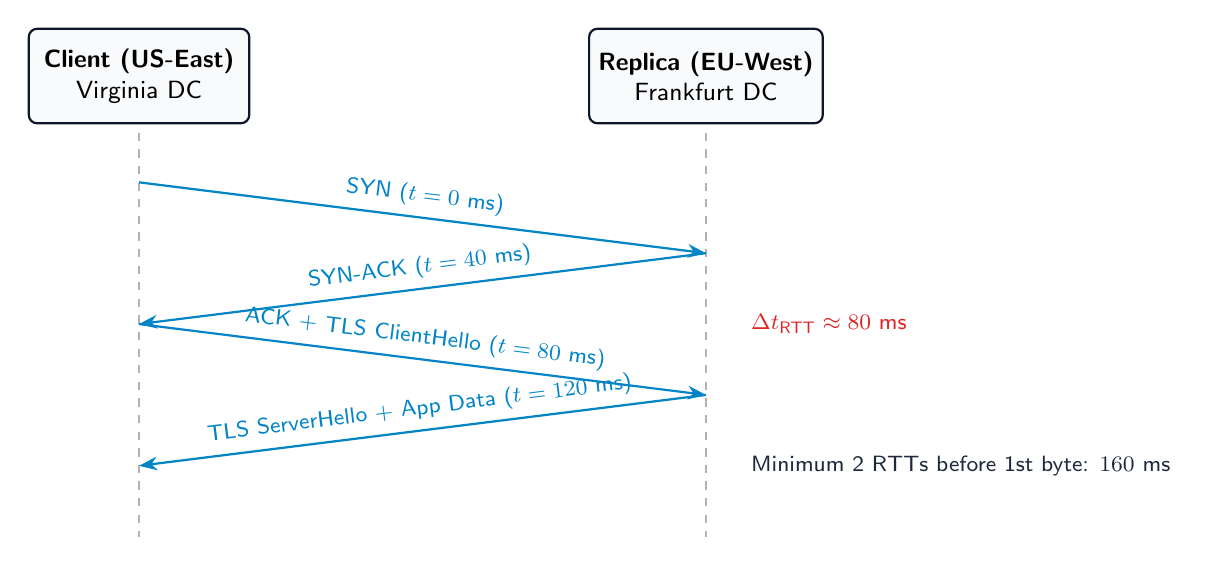
\begin{tikzpicture}[
  scale=0.9,
  node distance=2.5cm,
  server/.style={rectangle, draw=headingblue, fill=codebg, thick, rounded corners=3pt, minimum width=2.8cm, minimum height=1.2cm, align=center, font=\sffamily\small},
  timeline/.style={thick, dashed, color=gray!60},
  packet/.style={-{Stealth[scale=1.0]}, thick, color=linkblue}
]
  \node[server] (client) at (0, 0) {\textbf{Client (US-East)}\\Virginia DC};
  \node[server] (server) at (8, 0) {\textbf{Replica (EU-West)}\\Frankfurt DC};

  \draw[timeline] (0, -0.8) -- (0, -6.5);
  \draw[timeline] (8, -0.8) -- (8, -6.5);

  \draw[packet] (0, -1.5) -- node[above, sloped, font=\sffamily\footnotesize] {SYN ($t=0\text{ ms}$)} (8, -2.5);
  \draw[packet] (8, -2.5) -- node[above, sloped, font=\sffamily\footnotesize] {SYN-ACK ($t=40\text{ ms}$)} (0, -3.5);
  \draw[packet] (0, -3.5) -- node[above, sloped, font=\sffamily\footnotesize] {ACK + TLS ClientHello ($t=80\text{ ms}$)} (8, -4.5);
  \draw[packet] (8, -4.5) -- node[above, sloped, font=\sffamily\footnotesize] {TLS ServerHello + App Data ($t=120\text{ ms}$)} (0, -5.5);

  \node[anchor=west, font=\sffamily\footnotesize, color=warningRed] at (8.5, -3.5) {$\Delta t_{\text{RTT}} \approx 80\text{ ms}$};
  \node[anchor=west, font=\sffamily\footnotesize, color=textdark] at (8.5, -5.5) {Minimum 2 RTTs before 1st byte: $160\text{ ms}$};
\end{tikzpicture}
\caption{Cross-Datacenter TCP/TLS Handshake Latency Budget across Subsea Fiber}
\label{fig:cross-dc-latency}
\end{figure}

\begin{intuitionbox}[The Asymmetry of Local vs. Remote State]
On a single machine, reading from L1 cache takes $\sim 0.5\text{ ns}$, reading from main memory (DRAM) takes $\sim 100\text{ ns}$, and reading from an NVMe SSD takes $\sim 10\text{ to }50\ \mu\text{s}$. A cross-datacenter network packet takes $80\text{ ms} = 80{,}000{,}000\text{ ns}$. In relative terms, if an L1 cache reference took 1 second, a round-trip network packet across the Atlantic would take over 5 years.
\end{intuitionbox}

\subsection{The Fallacies of Distributed Computing}

In 1994, L. Peter Deutsch and James Gosling articulated the ``Eight Fallacies of Distributed Computing''. Every engineer designing distributed infrastructure must internalize these mistaken assumptions:
\begin{enumerate}[leftmargin=18pt]
  \item \textbf{The network is reliable}: Networks drop packets due to buffer overruns, fiber cuts, faulty transceivers, BGP route flaps, and switch reboots.
  \item \textbf{Latency is zero}: Network hops always incur physical transit and queuing delays.
  \item \textbf{Bandwidth is infinite}: While backbone links achieve Terabits per second, intra-rack switches and egress transit pipes saturate under burst traffic, causing tail latency spikes.
  \item \textbf{The network is secure}: Distributed packets transit multi-tenant infrastructure, middleboxes, and public backbones; encryption and integrity verification (TLS/mTLS) are mandatory.
  \item \textbf{Topology doesn't change}: Servers scale horizontally, IP addresses migrate, network interfaces fail, and cloud providers reroute virtual networks dynamically.
  \item \textbf{There is one administrator}: Heterogeneous systems span multiple administrative domains, authorization tiers, and cloud availability zones with divergent policies.
  \item \textbf{Transport cost is zero}: Serialization, deserialization, kernel-to-user-space context switching, memory copies, and cloud egress bandwidth charges represent non-trivial compute and monetary costs.
  \item \textbf{The network is homogeneous}: Workloads execute across distinct hardware generations, CPU architectures, operating system kernels, and NIC drivers.
\end{enumerate}

\section{Time, Clocks, and Ordering}

Single-node programs rely on monotonically increasing hardware counters or system clocks to order events. When an application writes record $A$ at $t_1$ and record $B$ at $t_2$, the condition $t_1 < t_2$ guarantees that $A$ occurred before $B$. In distributed systems, this assumption is invalid.

\subsection{Physical Clocks and Clock Drift}

Computer motherboards track time using quartz crystal oscillators. Quartz crystals vibrate at specific resonant frequencies when subjected to an electric field (the piezoelectric effect). However, manufacturing variations, ambient temperature fluctuations, and crystal aging cause drift.

A standard server quartz oscillator drifts by approximately 1 to 50 parts per million (ppm). A drift of 10 ppm accumulates:
\begin{equation}
10\ \mu\text{s/s} = 0.864\text{ seconds per day} \approx 26\text{ seconds per month}
\end{equation}

\subsection{Network Time Protocol (NTP) and Its Limits}

To mitigate drift, machines periodically synchronize their clocks with reference time sources using the Network Time Protocol (NTP). In NTP, a client exchanges UDP packets with a stratum-1 or stratum-2 time server.

Let a client send a request at client time $t_0$, received by the server at server time $t_1$. The server transmits its response at server time $t_2$, which reaches the client at client time $t_3$.

\begin{figure}[htbp]
\centering
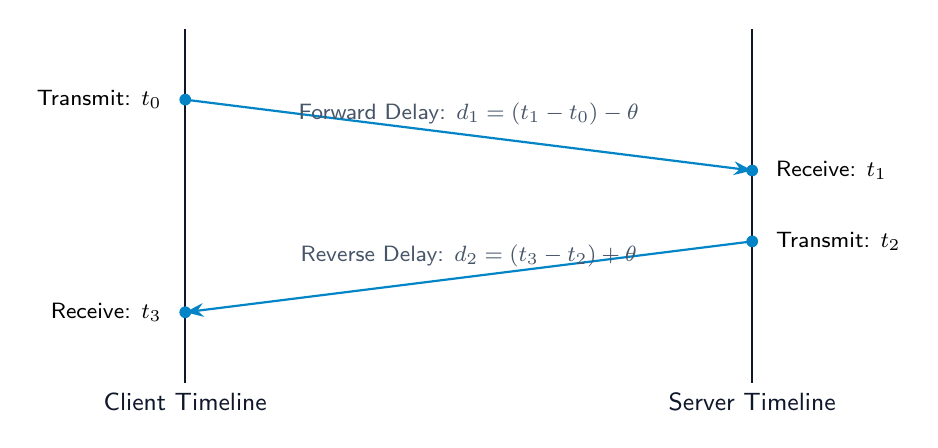
\begin{tikzpicture}[
  scale=0.9,
  timeline/.style={thick, color=headingblue},
  point/.style={circle, fill=linkblue, inner sep=1.5pt},
  packet/.style={-{Stealth[scale=1.0]}, thick, color=linkblue}
]
  \draw[timeline] (0, 0) -- (0, -5) node[below, font=\sffamily\small] {Client Timeline};
  \draw[timeline] (8, 0) -- (8, -5) node[below, font=\sffamily\small] {Server Timeline};

  \node[point] at (0, -1) {};
  \node[anchor=east, font=\sffamily\footnotesize] at (-0.2, -1) {Transmit: $t_0$};

  \node[point] at (8, -2) {};
  \node[anchor=west, font=\sffamily\footnotesize] at (8.2, -2) {Receive: $t_1$};

  \node[point] at (8, -3) {};
  \node[anchor=west, font=\sffamily\footnotesize] at (8.2, -3) {Transmit: $t_2$};

  \node[point] at (0, -4) {};
  \node[anchor=east, font=\sffamily\footnotesize] at (-0.2, -4) {Receive: $t_3$};

  \draw[packet] (0, -1) -- (8, -2);
  \draw[packet] (8, -3) -- (0, -4);

  \node[font=\sffamily\footnotesize, color=hoodSlate] at (4, -1.2) {Forward Delay: $d_1 = (t_1 - t_0) - \theta$};
  \node[font=\sffamily\footnotesize, color=hoodSlate] at (4, -3.2) {Reverse Delay: $d_2 = (t_3 - t_2) + \theta$};
\end{tikzpicture}
\caption{NTP Round-Trip Message Exchange and Clock Offset Calculation}
\label{fig:ntp-offset}
\end{figure}

The total round-trip network delay $\delta$ and clock offset $\theta$ are calculated as:
\begin{equation}
\delta = (t_3 - t_0) - (t_2 - t_1)
\end{equation}
\begin{equation}
\theta = \frac{(t_1 - t_0) + (t_2 - t_3)}{2}
\end{equation}

\begin{productionwarningbox}[The Asymmetry Fatal Flaw of NTP]
The offset formula strictly assumes that outbound network transit delay equals inbound transit delay ($d_1 = d_2$). If outbound network routing diverges from inbound routing (asymmetric BGP paths) or if outbound queuing differs from inbound queuing by $30\text{ ms}$, NTP will calculate an offset that is inaccurate by $15\text{ ms}$. Over the public Internet, NTP error commonly reaches $50\text{ ms}$ to $250\text{ ms}$. In virtualized cloud environments, VM hypervisor pauses, live migrations, and CPU throttling introduce artificial time dilation jumps of hundreds of milliseconds.
\end{productionwarningbox}

\subsection{Google TrueTime: Bounded Uncertainty}

To build Google Spanner---a globally distributed database offering external consistency without lock contention on read transactions---Google designed the TrueTime API.

Instead of exposing time as a discrete value ($t = \text{now}()$), TrueTime represents time as an interval $[t_{\text{earliest}}, t_{\text{latest}}]$ with guaranteed error bound $\varepsilon$:
\begin{equation}
\text{TrueTime.now}() \to [t_{\text{now}} - \varepsilon, t_{\text{now}} + \varepsilon]
\end{equation}

Google limits $\varepsilon$ to a small bound (typically $\le 7\text{ ms}$) by outfitting each datacenter with a dedicated time master cluster equipped with redundant GPS receivers and atomic rubidium clocks. If GPS fails or satellite signals are spoofed, the atomic clocks provide low-drift holdover timekeeping.

To ensure that transaction $T_1$ commit timestamp $s_1$ is strictly less than transaction $T_2$ commit timestamp $s_2$ whenever $T_2$ begins after $T_1$ commits, Spanner employs \textbf{commit wait}:

\begin{underthehoodbox}[Spanner's Commit Wait Rule]
When transaction $T_1$ prepares to commit, the coordinator picks absolute timestamp $s_1 = \text{TrueTime.now}().\text{latest}$. The coordinator refuses to release write locks or expose $T_1$'s mutated records to any client until it has paused for at least $2\varepsilon$:
\begin{equation}
\text{wait\_until}(\text{TrueTime.now}().\text{earliest} > s_1)
\end{equation}
This physical delay guarantees that any subsequent transaction $T_2$ will read $\text{TrueTime.now}().\text{earliest} > s_1$, mathematically enforcing linearizable ordering across global datacenters without cross-region coordination during read transactions.
\end{underthehoodbox}

\subsection{Lamport Logical Timestamps}

In 1978, Leslie Lamport published the seminal paper \emph{Time, Clocks, and the Ordering of Events in a Distributed System}, establishing that absolute physical time is unnecessary to order causally related events.

Lamport defined the \textbf{happens-before} relation ($\to$):
\begin{enumerate}[leftmargin=18pt]
  \item If event $a$ and event $b$ occur within the same process, and $a$ occurs before $b$, then $a \to b$.
  \item If event $a$ is the sending of a message by one process, and event $b$ is the receipt of that same message by another process, then $a \to b$.
  \item If $a \to b$ and $b \to c$, then $a \to c$ (transitivity).
\end{enumerate}

If neither $a \to b$ nor $b \to a$, the events are \textbf{concurrent} ($a \parallel b$).

\begin{lstlisting}[language=Python, caption={Implementation of a Lamport Logical Clock in Python}]
import threading

class LamportClock:
    def __init__(self, node_id: str):
        self.node_id = node_id
        self.counter = 0
        self._lock = threading.Lock()

    def tick(self) -> int:
        """Internal local event."""
        with self._lock:
            self.counter += 1
            return self.counter

    def send_event(self) -> int:
        """Invoked when dispatching a message over the network."""
        with self._lock:
            self.counter += 1
            return self.counter

    def receive_event(self, received_timestamp: int) -> int:
        """Invoked when receiving a message containing a remote timestamp."""
        with self._lock:
            self.counter = max(self.counter, received_timestamp) + 1
            return self.counter

    def compare(self, ts_a: int, node_a: str, ts_b: int, node_b: str) -> int:
        """Total order tie-breaking using unique node identifiers."""
        if ts_a < ts_b:
            return -1
        elif ts_a > ts_b:
            return 1
        else:
            return -1 if node_a < node_b else (1 if node_a > node_b else 0)
\end{lstlisting}

\begin{commonmistakebox}[Lamport Clocks Cannot Detect Concurrency]
A critical limitation of Lamport clocks is that while $a \to b \implies L(a) < L(b)$, the reverse is \textbf{not} true:
\begin{equation}
L(a) < L(b) \;\not\Longrightarrow\; a \to b
\end{equation}
If $L(a) = 3$ and $L(b) = 5$, it is impossible to determine whether $a$ caused $b$ or if $a$ and $b$ were completely concurrent events on isolated nodes. To detect and preserve concurrency, systems must use Vector Clocks.
\end{commonmistakebox}

\subsection{Vector Clocks}

A Vector Clock for a system of $N$ nodes is an array of $N$ logical integers: $V = [v_1, v_2, \dots, v_N]$. Node $i$ maintains its local vector $V_i$.

\textbf{Vector Clock Rules:}
\begin{enumerate}[leftmargin=18pt]
  \item Initially, all clock entries are zero: $V_i[j] = 0$ for all $j \in \{1, \dots, N\}$.
  \item Before node $i$ generates an internal or outbound event, it increments its own component:
  \begin{equation}
  V_i[i] \leftarrow V_i[i] + 1
  \end{equation}
  \item When node $i$ transmits a message, it attaches its current vector $V_i$.
  \item When node $j$ receives a message containing vector $V_{\text{msg}}$, it updates its clock:
  \begin{equation}
  V_j[k] \leftarrow \max(V_j[k], V_{\text{msg}}[k]) \quad \forall k \in \{1, \dots, N\}
  \end{equation}
  \begin{equation}
  V_j[j] \leftarrow V_j[j] + 1
  \end{equation}
\end{enumerate}

\textbf{Comparison and Causality Detection:}
\begin{itemize}[leftmargin=18pt]
  \item $V_A \le V_B \iff \forall k: V_A[k] \le V_B[k]$
  \item $V_A < V_B \iff (V_A \le V_B) \land (\exists k: V_A[k] < V_B[k])$
  \item If $V_A < V_B$, then $A$ causally preceded $B$ ($A \to B$).
  \item If neither $V_A \le V_B$ nor $V_B \le V_A$, then $A$ and $B$ are concurrent ($A \parallel B$). This indicates a conflict that must be resolved via application business logic (e.g., shopping cart merge) or Conflict-Free Replicated Data Types (CRDTs).
\end{itemize}

\begin{lstlisting}[language=Python, caption={Vector Clock Implementation with Conflict Detection in Python}]
from typing import Dict, Tuple

class VectorClock:
    def __init__(self, node_id: str):
        self.node_id = node_id
        self.clock: Dict[str, int] = {node_id: 0}

    def increment(self) -> Dict[str, int]:
        self.clock[self.node_id] = self.clock.get(self.node_id, 0) + 1
        return dict(self.clock)

    def update(self, remote_clock: Dict[str, int]) -> Dict[str, int]:
        # Merge by taking pairwise max
        for node, ts in remote_clock.items():
            self.clock[node] = max(self.clock.get(node, 0), ts)
        self.clock[self.node_id] = self.clock.get(self.node_id, 0) + 1
        return dict(self.clock)

    @staticmethod
    def compare(v1: Dict[str, int], v2: Dict[str, int]) -> str:
        """Returns: 'EQUAL', 'BEFORE', 'AFTER', or 'CONCURRENT'."""
        all_nodes = set(v1.keys()) | set(v2.keys())
        v1_greater = False
        v2_greater = False

        for node in all_nodes:
            val1 = v1.get(node, 0)
            val2 = v2.get(node, 0)
            if val1 > val2:
                v1_greater = True
            elif val2 > val1:
                v2_greater = True

        if v1_greater and not v2_greater:
            return "AFTER"       # v1 happened after v2
        elif v2_greater and not v1_greater:
            return "BEFORE"      # v1 happened before v2
        elif not v1_greater and not v2_greater:
            return "EQUAL"
        else:
            return "CONCURRENT"  # Conflict: both evolved independently!
\end{lstlisting}

\begin{realworldbox}[Amazon Dynamo and Riak Siblings]
Amazon DynamoDB's predecessor (the original 2007 Dynamo paper) and basho Riak utilized vector clocks to handle multi-master shopping cart writes during network partitions. When two datacenters were partitioned, a customer adding an item in California created vector $[CA:1, VA:0]$, while an item added in Virginia created $[CA:0, VA:1]$. Upon network recovery, comparing the two vectors returned \texttt{CONCURRENT}. Instead of discarding one write, the system preserved both entries as ``siblings'' and prompted the client application to union the items.
\end{realworldbox}

\section{Partial Failures and Theoretical Models}

In single-node software, components either execute or the operating system terminates the process (fail-stop). In distributed systems, failure is \textbf{partial}: some nodes continue operating normally while others crash, experience intermittent GC pauses, or become unreachable across broken network segments.

\subsection{Timing Models}

Theoretical distributed algorithms are proven under one of three fundamental timing assumptions:

\begin{table}[htbp]
\centering\small
\begin{tabular}{lp{4.2cm}p{4.2cm}p{3.8cm}}
\toprule
\textbf{Timing Model} & \textbf{Message Latency} & \textbf{Clock Drift} & \textbf{Real-World Feasibility} \\
\midrule
\textbf{Synchronous} & Strictly bounded: delay $\le D_{\text{max}}$ & Strictly bounded: drift $\le \rho$ & Specialized aerospace, avionics buses, hard real-time hardware. \\
\textbf{Asynchronous} & Unbounded: messages arrive eventually, no time limit & Clocks do not exist or drift arbitrarily & Most conservative theoretical model (FLM theorem applies). \\
\textbf{Partially Synchronous} & Asynchronous initially, but becomes bounded after an unknown Global Stabilization Time ($GST$) & Clocks drift, but drift becomes bounded after $GST$ & \textbf{Standard internet and cloud reality}; basis for Raft and Paxos. \\
\bottomrule
\end{tabular}
\caption{Distributed Systems Timing Models Comparison}
\label{tab:timing-models}
\end{table}

\subsection{Fault Models: Crash-Stop to Byzantine}

Node failure modes determine the complexity of consensus algorithms:

\begin{enumerate}[leftmargin=18pt]
  \item \textbf{Crash-Stop (Fail-Stop)}: A node operates correctly until it halts. Once halted, it never resumes or emits messages. Simplest model to reason about.
  \item \textbf{Crash-Recovery (Fail-Recovery)}: A node can halt at any time (e.g., kernel panic, power outage) and later reboot. When recovering, it retains state preserved on non-volatile storage (WAL, disk) but loses volatile RAM state. Raft and Paxos assume this model.
  \item \textbf{Omission Faults}: A node fails to transmit or receive messages due to full NIC buffers, dropped packets, or kernel socket exhaustion.
  \item \textbf{Byzantine Faults (Arbitrary Failures)}: Nodes may crash, drop messages, delay responses, forge cryptographic signatures, collude, or transmit intentionally conflicting data to different peers (split-brain sabotage). Common in blockchain and untrusted multi-party federations.
\end{enumerate}

\begin{figure}[htbp]
\centering
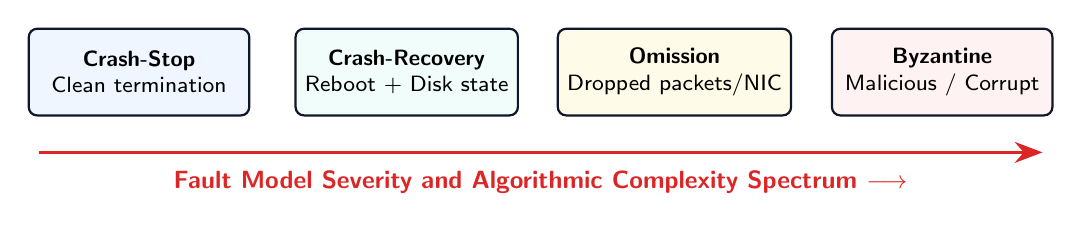
\begin{tikzpicture}[
  scale=0.85,
  box/.style={rectangle, draw=headingblue, fill=codebg, thick, rounded corners=3pt, minimum width=2.8cm, minimum height=1.1cm, align=center, font=\sffamily\footnotesize}
]
  \node[box, fill=exampleBg] (crash) at (0, 0) {\textbf{Crash-Stop}\\Clean termination};
  \node[box, fill=intuitionBg] (recovery) at (4, 0) {\textbf{Crash-Recovery}\\Reboot + Disk state};
  \node[box, fill=mistakeBg] (omission) at (8, 0) {\textbf{Omission}\\Dropped packets/NIC};
  \node[box, fill=warningBg] (byzantine) at (12, 0) {\textbf{Byzantine}\\Malicious / Corrupt};

  \draw[-{Stealth[scale=1.2]}, very thick, color=warningRed] (-1.5, -1.2) -- (13.5, -1.2)
    node[midway, below=3pt, font=\sffamily\small\bfseries] {Fault Model Severity and Algorithmic Complexity Spectrum $\longrightarrow$};
\end{tikzpicture}
\caption{Spectrum of Distributed Fault Models}
\label{fig:fault-spectrum}
\end{figure}

\begin{underthehoodbox}[The FLP Impossibility Result (Fischer, Lynch, Paterson 1985)]
The FLP theorem proves that in a fully \textbf{asynchronous} network model, no deterministic consensus protocol can guarantee both \textbf{Safety} (nothing bad happens, all nodes agree on the same value) and \textbf{Liveness} (something good happens eventually, nodes terminate and reach agreement) in the presence of even a \textbf{single unannounced crash-stop failure}.
Because it is impossible to distinguish between a crashed node and an arbitrarily slow node in an asynchronous model, protocols like Paxos and Raft trade off strict theoretical liveness: they ensure safety unconditionally under all network delays, but guarantee progress (liveness) only when the network transitions into a \textbf{partially synchronous} state.
\end{underthehoodbox}

\section{Summary \& Key Takeaways}
\begin{itemize}[leftmargin=18pt]
  \item Physical transmission speeds through optical fiber impose a strict latency floor of $\sim 4.89\ \mu\text{s/km}$, making zero-latency cross-region communication physically impossible.
  \item Physical wall clocks drift continuously due to thermal and mechanical oscillator variations. Public NTP cannot guarantee sub-millisecond precision due to asymmetric network delays.
  \item Google TrueTime solves absolute ordering by exposing an uncertainty interval $[t_{\text{now}} - \varepsilon, t_{\text{now}} + \varepsilon]$ and enforcing commit wait periods ($2\varepsilon$) backed by GPS receivers and atomic clocks.
  \item Lamport timestamps capture causality ($a \to b \implies L(a) < L(b)$) but cannot differentiate between causal and concurrent events.
  \item Vector clocks track independent node histories, allowing distributed systems to detect concurrent writes and data divergence.
  \item Real-world clouds operate under the \textbf{partially synchronous, crash-recovery} model. The FLP impossibility theorem proves that deterministic consensus in asynchronous networks must sacrifice unconditional liveness during network partitions.
\end{itemize}

\section{Exercises}

\subsection{Mechanics}
Given three nodes $A, B, C$ with initial vector clocks $[0, 0, 0]$:
\begin{enumerate}[leftmargin=18pt]
  \item Node $A$ executes an internal event $e_1$.
  \item Node $A$ sends message $m_1$ to Node $B$.
  \item Node $C$ executes an internal event $e_2$ independently.
  \item Node $B$ receives message $m_1$, then sends message $m_2$ to Node $C$.
  \item Node $C$ receives message $m_2$.
\end{enumerate}
Calculate the vector clock state at each event and determine whether event $e_2$ and the receipt of $m_1$ at Node $B$ are causal or concurrent.

\subsection{Debugging}
A financial audit log application records transactions using machine timestamps:
\begin{lstlisting}[language=Python]
record = {
    "account_id": acc_id,
    "delta": amount,
    "timestamp_ms": int(time.time() * 1000)
}
db.insert(record)
\end{lstlisting}
During a leap second insertion or hypervisor NTP step-adjustment, two debits of \$5,000 occur. The database deduplication engine uses \texttt{(account\_id, timestamp\_ms)} as a unique composite primary key. Explain the failure mode and provide a robust architectural fix.

\subsection{Architecture}
Design a distributed sequence ID generator (similar to Twitter Snowflake) capable of generating 100,000 globally unique, time-ordered 64-bit integers per second across 1,024 independent worker nodes without inter-node coordination during ID generation. Address clock backwards skew (NTP backward steps) explicitly.

\section{Detailed Solutions}

\subsection{Solution to Mechanics Exercise}
\begin{enumerate}[leftmargin=18pt]
  \item Node $A$ internal event $e_1$: Node $A$ increments its own index: $V_A = [1, 0, 0]$.
  \item Node $A$ sends $m_1$: increments $V_A = [2, 0, 0]$. Message carries vector $[2, 0, 0]$.
  \item Node $C$ internal event $e_2$: $V_C = [0, 0, 1]$.
  \item Node $B$ receives $m_1$: $V_B$ updates by taking max with $[2, 0, 0]$ and incrementing $B$'s slot: $V_B = [\max(0, 2), \max(0, 0) + 1, \max(0, 0)] = [2, 1, 0]$.
  \item Node $B$ sends $m_2$ to $C$: increments $V_B = [2, 2, 0]$. Message $m_2$ carries $[2, 2, 0]$.
  \item Node $C$ receives $m_2$: takes max with its current $[0, 0, 1]$ and increments $C$'s slot:
  $V_C = [\max(0, 2), \max(0, 2), \max(1, 0) + 1] = [2, 2, 2]$.
\end{enumerate}
\textbf{Causality evaluation:} Event $e_2$ has vector $[0, 0, 1]$. The receipt of $m_1$ at Node $B$ has vector $[2, 1, 0]$. Comparing the two: Node $A$'s and $B$'s components are greater in $B$'s vector, but Node $C$'s component is greater in $e_2$'s vector ($1 > 0$). Because neither vector dominates the other, $e_2 \parallel \text{receipt}(m_1)$ (\textbf{they are concurrent}).

\subsection{Solution to Debugging Exercise}
\textbf{Failure mode:} Physical wall clocks are not monotonic. When NTP steps backward (e.g., during clock slew adjustments or negative leap seconds), \texttt{time.time()} can return identical or decreasing values. If two debits occur during this window, the second debit will trigger a composite primary key collision (\texttt{UniqueViolationException}) and be rejected, or overwrite the prior record if an \texttt{UPSERT} pattern is used.
\textbf{Architectural fix:}
1. Never use wall-clock time as a primary key or unique identifier.
2. In single processes, use monotonic hardware timers (\texttt{time.monotonic\_ns()} in Python, \texttt{CLOCK\_MONOTONIC} in Linux).
3. Combine monotonic time with a node identifier and an auto-incrementing atomic sequence counter (e.g., Snowflake ID format: 41 bits timestamp, 10 bits worker ID, 12 bits sequence number).
4. Configure local NTP daemons with \textbf{clock slewing only} (passing \texttt{-x} to \texttt{ntpd} or configuring \texttt{chrony} with \texttt{makestep 0}) to forbid hard backward step jumps.

\subsection{Solution to Architecture Exercise}
\textbf{Bit Allocation Layout (64-bit integer):}
\begin{itemize}[leftmargin=18pt]
  \item \textbf{1 bit sign}: Always 0 (keeps integers positive).
  \item \textbf{41 bits millisecond timestamp}: Difference from custom epoch (e.g., Jan 1, 2026). Yields $(2^{41} - 1) / (1000 \times 3600 \times 24 \times 365) \approx 69.7$ years of lifespan.
  \item \textbf{10 bits worker/machine ID}: Supports up to $2^{10} = 1{,}024$ distinct worker instances. Assigned via ZooKeeper, Consul, or K8s StatefulSet pod ordinal index.
  \item \textbf{12 bits sequence counter}: Supports $2^{12} = 4{,}096$ IDs per millisecond per node ($4{,}096{,}000$ IDs/second per worker, well beyond the 100k requirement).
\end{itemize}

\textbf{Handling Clock Backward Skew:}
\begin{lstlisting}[language=Python]
class SnowflakeGenerator:
    def __init__(self, worker_id: int, epoch: int = 1767225600000):
        assert 0 <= worker_id < 1024
        self.worker_id = worker_id
        self.epoch = epoch
        self.sequence = 0
        self.last_timestamp = -1

    def next_id(self) -> int:
        current_time = self._current_ms()

        # Handle backward clock drift
        if current_time < self.last_timestamp:
            drift = self.last_timestamp - current_time
            if drift < 5:  # Tolerate small drift (<5ms) by spinning
                while current_time < self.last_timestamp:
                    time.sleep(0.001)
                    current_time = self._current_ms()
            else:
                raise SystemClockException(f"Clock moved backwards by {drift}ms")

        if current_time == self.last_timestamp:
            self.sequence = (self.sequence + 1) & 0xFFF
            if self.sequence == 0:
                # Sequence exhausted for this millisecond; spin wait
                while current_time <= self.last_timestamp:
                    current_time = self._current_ms()
        else:
            self.sequence = 0

        self.last_timestamp = current_time
        return ((current_time - self.epoch) << 22) | (self.worker_id << 12) | self.sequence

    def _current_ms(self) -> int:
        return int(time.time() * 1000)
\end{lstlisting}

\section{Further Reading \& Citations}
\begin{itemize}[leftmargin=18pt]
  \item Lamport, L. (1978). \emph{Time, clocks, and the ordering of events in a distributed system}. Communications of the ACM, 21(7), 558--565.
  \item Corbett, J. C., et al. (2013). \emph{Spanner: Google's globally distributed database}. ACM Transactions on Computer Systems (TOCS), 31(3), 1--22.
  \item Fischer, M. J., Lynch, N. A., \& Paterson, M. S. (1985). \emph{Impossibility of distributed consensus with one faulty process}. Journal of the ACM (JACM), 32(2), 374--382.
  \item Deutsch, L. P. (1994). \emph{The Eight Fallacies of Distributed Computing}. Sun Microsystems Technical Report.
\end{itemize}

\chapter{CAP Theorem and Consistency Models}
\label{ch:cap-consistency}

\begin{chaptergoalsbox}
\textbf{What you will learn:}
\begin{itemize}[leftmargin=12pt]
  \item The formal formulation and mathematical proof of Eric Brewer's CAP Theorem (Gilbert \& Lynch 2002).
  \item Why ``pick any two'' is a dangerous myth: network partitions are unavoidable physical events ($P$ is non-negotiable).
  \item Daniel Abadi's PACELC Theorem: modeling the trade-off between Consistency/Availability during partitions, and Latency/Consistency during normal operation.
  \item The complete consistency spectrum: Strict Serializability, Linearizability, Sequential Consistency, Causal Consistency, Read-Your-Writes, and Eventual Consistency.
  \item The Raft Consensus Algorithm: leader election, log replication safety invariants, joint consensus cluster membership changes, and log compaction.
\end{itemize}

\textbf{What you should already understand:}
\begin{itemize}[leftmargin=12pt]
  \item Distributed timing models and vector clocks from Chapter~\ref{ch:distributed-fundamentals}.
  \item Client-server state replication and remote procedure calls (RPC).
\end{itemize}

\textbf{Why this topic exists:}
When network links between servers break, systems cannot magically maintain both instantaneous global consistency and 100\% availability. Understanding consistency models allows engineers to select the exact level of correctness required without paying unnecessary latency penalties.

\textbf{Motivating practical problem:}
An online social gaming platform stores player inventory across multi-region Cassandra nodes configured with \texttt{ANY} write consistency to maximize availability. During a cross-Atlantic link degradation, players discover they can duplicate high-value virtual weapons by trading simultaneously from two browser windows connected to different regional data centers.
\end{chaptergoalsbox}

\section{The CAP Theorem: Formalization and Reality}

In 2000, Eric Brewer presented the CAP conjecture at the Symposium on Principles of Distributed Computing (PODC). In 2002, Seth Gilbert and Nancy Lynch published a formal mathematical proof of the conjecture under an asynchronous network model.

\subsection{Formal Definitions (Gilbert \& Lynch)}

To understand CAP, one must reject colloquial definitions of its terms:

\begin{enumerate}[leftmargin=18pt]
  \item \textbf{Consistency ($C$)}: Gilbert and Lynch strictly equate Consistency with \textbf{Linearizability} (atomic or external consistency). Every read operation must return the value of the most recent write, or an error. Once a read returns a new value $v$, all subsequent reads (by any client across the entire cluster) must return $v$ or a strictly newer value.
  \item \textbf{Availability ($A$)}: Every non-failing node must return a non-error response to every request it receives. Returning a timeout, an HTTP 500 error, or an explicit exception violates availability under the formal CAP definition.
  \item \textbf{Partition Tolerance ($P$)}: The system continues to operate despite an arbitrary number of messages being dropped or delayed by the network between nodes.
\end{enumerate}

\subsection{The Impossibility Proof}

Consider a minimal distributed system consisting of two nodes, $G_1$ and $G_2$, maintaining a single integer variable $v$, initially $0$.

\begin{figure}[htbp]
\centering
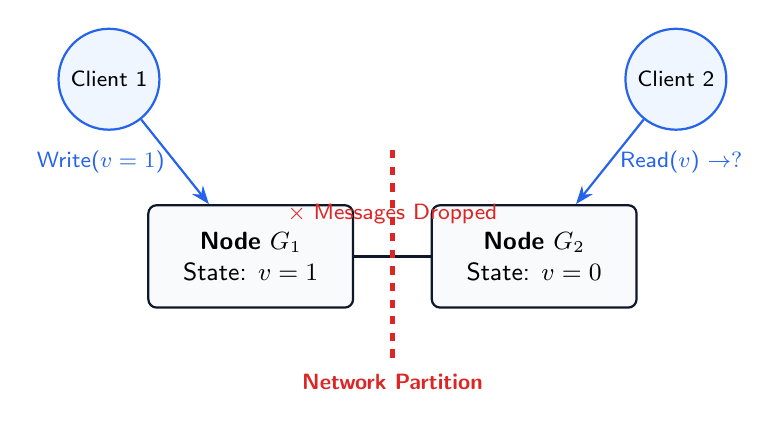
\begin{tikzpicture}[
  scale=0.9,
  server/.style={rectangle, draw=headingblue, fill=codebg, thick, rounded corners=3pt, minimum width=2.6cm, minimum height=1.3cm, align=center, font=\sffamily\small},
  client/.style={circle, draw=exampleBlue, fill=exampleBg, thick, minimum size=1.0cm, align=center, font=\sffamily\footnotesize},
  line/.style={thick, color=headingblue},
  partition/.style={ultra thick, dashed, color=warningRed}
]
  \node[client] (c1) at (-4, 1.5) {Client 1};
  \node[client] (c2) at (4, 1.5) {Client 2};

  \node[server] (g1) at (-2, -1) {\textbf{Node $G_1$}\\State: $v=1$};
  \node[server] (g2) at (2, -1) {\textbf{Node $G_2$}\\State: $v=0$};

  \draw[-{Stealth[scale=1.0]}, thick, color=exampleBlue] (c1) -- node[left, font=\sffamily\footnotesize] {Write($v=1$)} (g1);
  \draw[-{Stealth[scale=1.0]}, thick, color=exampleBlue] (c2) -- node[right, font=\sffamily\footnotesize] {Read($v$) $\to ?$} (g2);

  \draw[line] (g1) -- (g2);
  \draw[partition] (0, 0.5) -- (0, -2.5) node[below, font=\sffamily\bfseries\footnotesize, color=warningRed] {Network Partition};

  \node[font=\sffamily\footnotesize, color=warningRed] at (0, -0.4) {$\times$ Messages Dropped};
\end{tikzpicture}
\caption{The Fundamental CAP Partition Dilemma between Nodes $G_1$ and $G_2$}
\label{fig:cap-proof}
\end{figure}

Assume a network partition occurs between $G_1$ and $G_2$: no message sent by $G_1$ can reach $G_2$, and vice versa.
\begin{enumerate}[leftmargin=18pt]
  \item Client 1 connects to $G_1$ and executes $\text{Write}(v=1)$.
  \item Because $G_1$ is non-failing and the system is claimed to be \textbf{Available}, $G_1$ must acknowledge the write with success.
  \item $G_1$ attempts to replicate the update to $G_2$, but all sync messages are dropped by the partition.
  \item Client 2 connects to $G_2$ and executes $\text{Read}(v)$.
  \item $G_2$ faces an inescapable dilemma:
  \begin{itemize}[leftmargin=12pt]
    \item If $G_2$ responds with $v=0$ (its local state), it violates \textbf{Consistency} (Linearizability), because Client 1's write of $1$ completed before Client 2's read began.
    \item If $G_2$ blocks, waits for the partition to heal, or returns an error, it violates \textbf{Availability}.
  \end{itemize}
\end{enumerate}
Therefore, no distributed system can achieve both Linearizability and Availability in the presence of a network partition.

\begin{productionwarningbox}[The Myth of ``CA'' Systems]
In marketing literature, some relational databases claim to be ``CA'' (Consistent and Available). This is mathematically false in any distributed environment. Network partitions are physical phenomena caused by severed cables, failed top-of-rack switches, or saturated interfaces. You cannot ``choose'' not to have partitions.
Thus, the true choice is binary:
\begin{itemize}[leftmargin=12pt]
  \item \textbf{CP}: Choose Consistency by refusing writes or failing reads on partitioned nodes.
  \item \textbf{AP}: Choose Availability by serving stale local data or accepting divergent writes that must be reconciled later.
\end{itemize}
\end{productionwarningbox}

\section{The PACELC Theorem}

While CAP describes system behavior \textbf{during rare network partitions}, systems spend 99.99\% of their lifecycle operating normally without partitions. In 2012, Daniel Abadi introduced the PACELC theorem to describe the full design trade-off space:

\begin{equation}
\mathbf{If\ Partition\ (P)} \implies \text{Choose between } \mathbf{Availability\ (A)} \text{ and } \mathbf{Consistency\ (C)}
\end{equation}
\begin{equation}
\mathbf{Else\ (E)} \implies \text{Choose between } \mathbf{Latency\ (L)} \text{ and } \mathbf{Consistency\ (C)}
\end{equation}

\begin{table}[htbp]
\centering\small
\begin{tabular}{lllp{6.0cm}}
\toprule
\textbf{System} & \textbf{Partition Mode} & \textbf{Normal Mode} & \textbf{Architectural Mechanics} \\
\midrule
\textbf{Spanner / CockroachDB} & CP & PC & Replicated state machine via Raft/Paxos. Enforces strict consistency; pays WAN round-trip latency on normal writes. \\
\textbf{Cassandra / DynamoDB} & AP & PA / EL & Defaults to eventual consistency. Writes to local quorum; returns quickly without waiting for cross-region consensus. \\
\textbf{MongoDB (w:majority)} & CP & PC & Routes all writes to primary replica. Rejects writes if primary is partitioned away from majority. \\
\textbf{VoltDB / H-Store} & CP & PC & Strict ACID partitioned memory. Halts transaction processing during replica disconnects. \\
\bottomrule
\end{tabular}
\caption{Classification of Distributed Data Stores under the PACELC Theorem}
\label{tab:pacelc}
\end{table}

\begin{intuitionbox}[The Latency-Consistency Trade-Off (PC/EC)]
Even when all fiber cables are intact and routers are healthy, enforcing Linearizability requires a node to coordinate with a quorum of replicas before answering a write or read request. This cross-node coordination adds round-trip network latency. If an application chooses low latency (EL), it must return the local node's current value immediately, accepting that the data might be milliseconds out of date.
\end{intuitionbox}

\section{The Consistency Spectrum}

Consistency is not a binary choice between ``strong'' and ``eventual''. It is a continuous hierarchy of formal guarantees.

\begin{figure}[htbp]
\centering
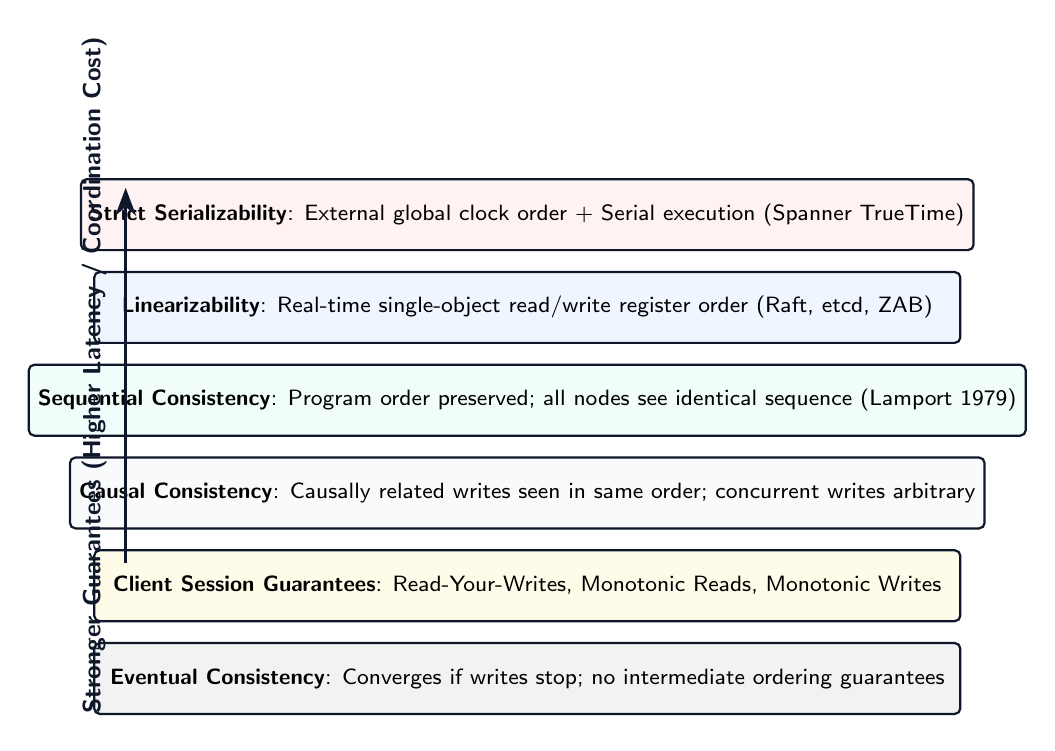
\begin{tikzpicture}[
  scale=0.85,
  level/.style={rectangle, draw=headingblue, fill=codebg, thick, rounded corners=2pt, minimum width=11cm, minimum height=0.9cm, align=left, font=\sffamily\footnotesize}
]
  \node[level, fill=warningBg] (s-ser) at (0, 0) {\textbf{Strict Serializability}: External global clock order + Serial execution (Spanner TrueTime)};
  \node[level, fill=exampleBg, below=0.25cm of s-ser] (lin) {\textbf{Linearizability}: Real-time single-object read/write register order (Raft, etcd, ZAB)};
  \node[level, fill=intuitionBg, below=0.25cm of lin] (seq) {\textbf{Sequential Consistency}: Program order preserved; all nodes see identical sequence (Lamport 1979)};
  \node[level, fill=hoodBg, below=0.25cm of seq] (causal) {\textbf{Causal Consistency}: Causally related writes seen in same order; concurrent writes arbitrary};
  \node[level, fill=mistakeBg, below=0.25cm of causal] (session) {\textbf{Client Session Guarantees}: Read-Your-Writes, Monotonic Reads, Monotonic Writes};
  \node[level, fill=gray!10, below=0.25cm of session] (eventual) {\textbf{Eventual Consistency}: Converges if writes stop; no intermediate ordering guarantees};

  \draw[-{Stealth[scale=1.2]}, very thick, color=headingblue] (-6.0, -5.2) -- (-6.0, 0.4)
    node[midway, sloped, above=3pt, font=\sffamily\small\bfseries] {Stronger Guarantees (Higher Latency / Coordination Cost)};
\end{tikzpicture}
\caption{The Consistency Model Hierarchy from Eventual to Strict Serializability}
\label{fig:consistency-spectrum}
\end{figure}

\subsection{Linearizability vs. Serializability}

A common source of confusion in database engineering is conflating Linearizability and Serializability:
\begin{itemize}[leftmargin=18pt]
  \item \textbf{Serializability} is a multi-operation, multi-object transaction property. It guarantees that the execution of a set of concurrent transactions produces an outcome equivalent to \emph{some} sequential execution order. However, it imposes \textbf{no real-time constraint}. A serializable database could legally return data from yesterday, provided all historical transactions are ordered consistently.
  \item \textbf{Linearizability} is a composable, real-time property of individual operations on single objects. It guarantees that if operation $B$ starts after operation $A$ finishes in physical wall-clock time, operation $B$ must observe the state left by $A$ or a subsequent operation.
  \item \textbf{Strict Serializability (External Consistency)} is the union of both: transactions execute serializably, and their execution order respects physical real-time precedence.
\end{itemize}

\subsection{Causal Consistency and Session Guarantees}

For systems that cannot afford the latency of Linearizability, Causal Consistency represents the strongest model achievable in a completely available (AP) partition-tolerant system (Mahajan et al., 2011).

In web architectures, four \textbf{Client Session Guarantees} provide predictable semantics without requiring full consensus:
\begin{enumerate}[leftmargin=18pt]
  \item \textbf{Read-Your-Writes}: A client always sees its own previous updates. Implemented by sticky sessions, routing reads to the master node for $T$ seconds after a write, or caching client writes in browser local storage.
  \item \textbf{Monotonic Reads}: If a client reads value $v_1$ at time $t_1$, any subsequent read at $t_2 > t_1$ will never return an older state $v_0$. Prevents time-traveling user interfaces.
  \item \textbf{Monotonic Writes}: A client's writes are applied in the exact order they were submitted.
  \item \textbf{Writes-Follow-Reads}: If a client reads state $v$ and subsequently writes $v'$, any other client observing $v'$ will also observe $v$.
\end{enumerate}

\section{The Raft Consensus Algorithm}

Designed by Diego Ongaro and John Ousterhout (Stanford, 2014), Raft is an understandable consensus algorithm equivalent to Paxos in fault tolerance and performance. Raft decomposes consensus into three independent subproblems:
\begin{enumerate}[leftmargin=18pt]
  \item \textbf{Leader Election}: Selecting one server to manage the replicated log.
  \item \textbf{Log Replication}: Accepting log entries from clients, replicating them across followers, and maintaining consistency.
  \item \textbf{Safety}: Enforcing that if any server commits a log entry at a specific index, no other server will ever apply a different log entry for that index.
\end{enumerate}

\subsection{State Machine Replication}

Raft implements \textbf{State Machine Replication (SMR)}. Identical state machines (such as a key-value store) execute on $2F + 1$ servers. The state machines process an identical sequence of inputs from an ordered write-ahead log (WAL), guaranteeing that all non-failing nodes produce identical output states.

\begin{figure}[htbp]
\centering
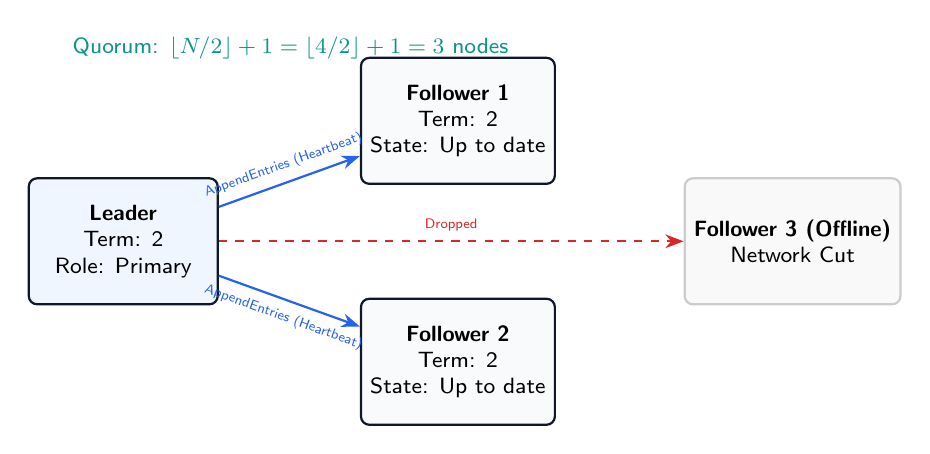
\begin{tikzpicture}[
  scale=0.85,
  node distance=1.5cm,
  nodebox/.style={rectangle, draw=headingblue, fill=codebg, thick, rounded corners=3pt, minimum width=2.4cm, minimum height=1.6cm, align=center, font=\sffamily\footnotesize}
]
  \node[nodebox, fill=exampleBg] (leader) at (0, 0) {\textbf{Leader}\\Term: 2\\Role: Primary};
  \node[nodebox] (f1) at (5, 1.8) {\textbf{Follower 1}\\Term: 2\\State: Up to date};
  \node[nodebox] (f2) at (5, -1.8) {\textbf{Follower 2}\\Term: 2\\State: Up to date};
  \node[nodebox, draw=gray!40, fill=gray!5] (f3) at (10, 0) {\textbf{Follower 3 (Offline)}\\Network Cut};

  \draw[-{Stealth[scale=1.0]}, thick, color=exampleBlue] (leader) -- node[above, sloped, font=\sffamily\tiny] {AppendEntries (Heartbeat)} (f1);
  \draw[-{Stealth[scale=1.0]}, thick, color=exampleBlue] (leader) -- node[below, sloped, font=\sffamily\tiny] {AppendEntries (Heartbeat)} (f2);
  \draw[-{Stealth[scale=1.0]}, thick, dashed, color=warningRed] (leader) -- node[above, font=\sffamily\tiny] {Dropped} (f3);

  \node[anchor=north, font=\sffamily\footnotesize, color=intuitionTeal] at (2.5, 3.2) {Quorum: $\lfloor N/2 \rfloor + 1 = \lfloor 4/2 \rfloor + 1 = 3$ nodes};
\end{tikzpicture}
\caption{Raft Cluster Topology with Majority Quorum ($N=4$, Quorum=3)}
\label{fig:raft-topology}
\end{figure}

\subsection{Leader Election Mechanics}

Nodes exist in one of three states: \textbf{Follower}, \textbf{Candidate}, or \textbf{Leader}.
Time is divided into arbitrary terms identified by monotonic integers.

\begin{figure}[htbp]
\centering
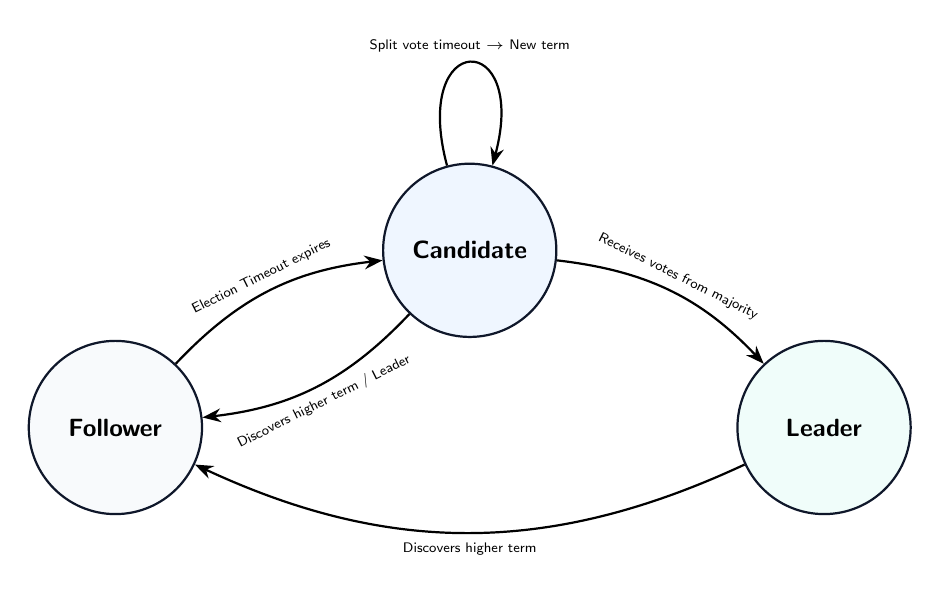
\begin{tikzpicture}[
  scale=0.9,
  state/.style={circle, draw=headingblue, fill=codebg, thick, minimum size=2.2cm, align=center, font=\sffamily\small}
]
  \node[state] (f) at (0, 0) {\textbf{Follower}};
  \node[state, fill=exampleBg] (c) at (5, 2.5) {\textbf{Candidate}};
  \node[state, fill=intuitionBg] (l) at (10, 0) {\textbf{Leader}};

  \draw[-{Stealth[scale=1.0]}, thick] (f) to [bend left=20] node[above, sloped, font=\sffamily\tiny] {Election Timeout expires} (c);
  \draw[-{Stealth[scale=1.0]}, thick] (c) to [bend left=20] node[above, sloped, font=\sffamily\tiny] {Receives votes from majority} (l);
  \draw[-{Stealth[scale=1.0]}, thick] (l) to [bend left=25] node[below, sloped, font=\sffamily\tiny] {Discovers higher term} (f);
  \draw[-{Stealth[scale=1.0]}, thick] (c) to [bend left=20] node[below, sloped, font=\sffamily\tiny] {Discovers higher term / Leader} (f);
  \draw[-{Stealth[scale=1.0]}, thick] (c) to [loop above] node[above, font=\sffamily\tiny] {Split vote timeout $\to$ New term} (c);
\end{tikzpicture}
\caption{Raft Finite State Machine Transitions}
\label{fig:raft-fsm}
\end{figure}

\textbf{Randomized Election Timeouts:} To prevent split-vote deadlocks where multiple candidates split votes evenly, Raft randomizes election timeouts between $150\text{ ms}$ and $300\text{ ms}$. The first node whose timer expires increments its term, transitions to Candidate, votes for itself, and broadcasts \texttt{RequestVote} RPCs.

\subsection{Log Matching and Election Safety Invariant}

Raft enforces strict invariants:
\begin{enumerate}[leftmargin=18pt]
  \item \textbf{Election Safety}: At most one leader can be elected in a given term.
  \item \textbf{Leader Append-Only}: A leader never overwrites or truncates its own log entries; it only appends new entries.
  \item \textbf{Log Matching Property}: If two logs contain an entry with the same index and term, then:
  \begin{itemize}[leftmargin=12pt]
    \item They store the same command.
    \item Their logs are completely identical in all preceding entries from index 1 to that index.
  \end{itemize}
  \item \textbf{Leader Completeness}: If a log entry is committed in a given term, that entry will be present in the logs of the leaders for all higher-numbered terms.
\end{enumerate}

\begin{underthehoodbox}[How Raft Enforces Leader Completeness without Transferring Old Logs]
Unlike Multi-Paxos, which allows a new leader to be elected with an incomplete log and then retroactively discovers committed entries, Raft strictly forbids a node from becoming leader if it lacks any committed entries.
When a voter evaluates a \texttt{RequestVote} RPC containing Candidate $(\text{term}_c, \text{lastLogIndex}_c, \text{lastLogTerm}_c)$, it rejects the vote unless the candidate's log is at least as up-to-date as its own:
\begin{equation}
(\text{lastLogTerm}_c > \text{lastLogTerm}_v) \lor (\text{lastLogTerm}_c == \text{lastLogTerm}_v \land \text{lastLogIndex}_c \ge \text{lastLogIndex}_v)
\end{equation}
Because any committed entry must reside on a majority of nodes, and an elected candidate must obtain votes from a majority of nodes, the candidate's quorum and the commit quorum must overlap by at least one node. That overlapping node will refuse to vote for any candidate lacking the committed entry.
\end{underthehoodbox}

\begin{lstlisting}[language=Python, caption={Core Raft Log Replication RPC Handler in Python}]
from typing import List, Optional

class LogEntry:
    def __init__(self, term: int, index: int, command: str):
        self.term = term
        self.index = index
        self.command = command

class RaftFollower:
    def __init__(self, node_id: str):
        self.node_id = node_id
        self.current_term = 0
        self.voted_for: Optional[str] = None
        self.log: List[LogEntry] = [LogEntry(0, 0, "INIT")] # 1-based indexing
        self.commit_index = 0

    def handle_append_entries(
        self,
        leader_term: int,
        leader_id: str,
        prev_log_index: int,
        prev_log_term: int,
        entries: List[LogEntry],
        leader_commit: int
    ) -> (int, bool):
        # Rule 1: Reply false if term < current_term
        if leader_term < self.current_term:
            return self.current_term, False

        # Update local term if leader is newer
        if leader_term > self.current_term:
            self.current_term = leader_term
            self.voted_for = None

        # Rule 2: Reply false if log doesn't contain entry at prev_log_index with prev_log_term
        if prev_log_index >= len(self.log):
            return self.current_term, False
        if self.log[prev_log_index].term != prev_log_term:
            # Conflict detected: follower log differs from leader!
            return self.current_term, False

        # Rule 3: If existing entry conflicts with new one, delete existing entry and all following
        insert_index = prev_log_index + 1
        for entry in entries:
            if insert_index < len(self.log):
                if self.log[insert_index].term != entry.term:
                    self.log = self.log[:insert_index] # Truncate conflicting suffix
                    self.log.append(entry)
            else:
                self.log.append(entry)
            insert_index += 1

        # Rule 4: Update commit index
        if leader_commit > self.commit_index:
            self.commit_index = min(leader_commit, len(self.log) - 1)

        return self.current_term, True
\end{lstlisting}

\section{Summary \& Key Takeaways}
\begin{itemize}[leftmargin=18pt]
  \item The CAP Theorem formally proves that an asynchronous network cannot simultaneously provide Linearizability ($C$) and 100\% non-failing availability ($A$) during network partitions ($P$).
  \item Network partitions are an inescapable physical reality in WANs and cloud networks; systems must be designed explicitly as CP or AP.
  \item The PACELC Theorem expands CAP to normal operations: if partitioned ($P$), trade Consistency ($C$) vs. Availability ($A$); else ($E$), trade Latency ($L$) vs. Consistency ($C$).
  \item Consistency is a spectrum: Strict Serializability $\to$ Linearizability $\to$ Sequential $\to$ Causal $\to$ Read-Your-Writes $\to$ Eventual.
  \item Linearizability governs single-operation real-time boundaries, whereas Serializability governs multi-operation transaction isolation.
  \item Raft solves consensus via State Machine Replication, using randomized election timers, leader log matching invariants, and majority quorum validation.
\end{itemize}

\section{Exercises}

\subsection{Mechanics}
Consider a Raft cluster of 5 nodes ($N_1, N_2, N_3, N_4, N_5$). The cluster is partitioned into two subnets: $\{N_1, N_2\}$ and $\{N_3, N_4, N_5\}$.
\begin{enumerate}[leftmargin=18pt]
  \item Can the partition containing $\{N_1, N_2\}$ elect a new leader? Show the quorum calculation.
  \item Can the partition containing $\{N_3, N_4, N_5\}$ elect a new leader and commit new client writes?
  \item Suppose $N_1$ was the leader before the partition. What happens when a client submits write $W_A$ to $N_1$, and another client submits write $W_B$ to the newly elected leader in the majority partition?
\end{enumerate}

\subsection{Debugging}
An engineer configures an Elasticsearch cluster with 3 master-eligible nodes. To prevent split-brain during network partitions, the legacy setting \texttt{discovery.zen.minimum\_master\_nodes} must be specified. The engineer sets this value to \texttt{1}. Explain the exact sequence of events during a switch failure that results in data corruption and loss.

\subsection{Architecture}
You are designing a globally distributed collaborative document editor (like Google Docs or Figma). Users in Tokyo and New York must edit the same text block simultaneously with zero input latency. Detail why a CP consensus model (like Raft or Spanner) is inappropriate for real-time keystroke processing, and architect a solution using Conflict-Free Replicated Data Types (CRDTs) or Operational Transformation (OT).

\section{Detailed Solutions}

\subsection{Solution to Mechanics Exercise}
\begin{enumerate}[leftmargin=18pt]
  \item In a 5-node cluster, a majority quorum requires $\lfloor 5/2 \rfloor + 1 = 3$ votes. The partition $\{N_1, N_2\}$ contains only 2 nodes. Even if both vote for the same candidate, $2 < 3$. Therefore, this partition cannot elect a leader.
  \item The partition $\{N_3, N_4, N_5\}$ contains 3 nodes. Because $3 \ge 3$, they constitute a majority quorum. They can elect a new leader (e.g., $N_3$) and successfully commit client writes by replicating to each other.
  \item When Client 1 submits $W_A$ to $N_1$, $N_1$ writes $W_A$ to its local log and dispatches \texttt{AppendEntries} to $N_2$. $N_2$ appends it, but $N_1$ cannot reach $N_3, N_4, N_5$. Because $N_1$ only gathers 2 acknowledgments (itself and $N_2$), it cannot commit $W_A$. It must either block or return a timeout to Client 1. Meanwhile, the leader in the majority partition receives $W_B$, replicates it to 3 nodes ($N_3, N_4, N_5$), commits it, and returns success to Client 2.
  When the partition heals, the new leader sends \texttt{AppendEntries} to $N_1$ and $N_2$ with a higher term. $N_1$ steps down to Follower, and its uncommitted entry $W_A$ is overwritten and truncated by the leader's log.
\end{enumerate}

\subsection{Solution to Debugging Exercise}
\textbf{The Split-Brain Failure Mode:}
When \texttt{minimum\_master\_nodes} is set to 1 in a 3-node cluster:
\begin{enumerate}[leftmargin=18pt]
  \item Suppose a network partition separates Node $A$ from Nodes $B$ and $C$.
  \item Node $A$ detects the loss of heartbeats, increments its term, and solicits votes. Because its threshold is $\ge 1$, Node $A$ votes for itself, reaches the threshold of 1, and declares itself active Master for the cluster.
  \item Simultaneously, Nodes $B$ and $C$ elect Node $B$ as Master.
  \item Clients routed to Node $A$ (via DNS round-robin or local load balancers) execute index and update operations on Node $A$.
  \item Other clients execute updates on Node $B$.
  \item Both nodes independently allocate document IDs, delete indices, and advance internal version counters along divergent timelines.
  \item When the network heals, neither master will step down cleanly. If one is forcibly reconciled over the other, all writes accepted by the deposed master are silently and permanently deleted.
\end{enumerate}
\textbf{The Correct Rule:} The minimum master nodes must always satisfy $\lfloor N/2 \rfloor + 1$. For 3 nodes, this value must be 2. In modern Elasticsearch (v7+), the Raft-based cluster coordination subsystem handles this automatically.

\subsection{Solution to Architecture Exercise}
\textbf{Why CP / Raft is Inappropriate:}
A CP consensus protocol requires a synchronous round-trip to a majority quorum for every single operation before acknowledging it to the client. At a physical speed of light latency of $80\text{ ms}$ to $120\text{ ms}$ between Tokyo and New York, a user typing at 60 words per minute would experience noticeable input lag on every keystroke. Furthermore, if a user goes through an airplane tunnel or loses WiFi, a CP system rejects all edits.

\textbf{CRDT-Based Architecture:}
\begin{figure}[htbp]
\centering
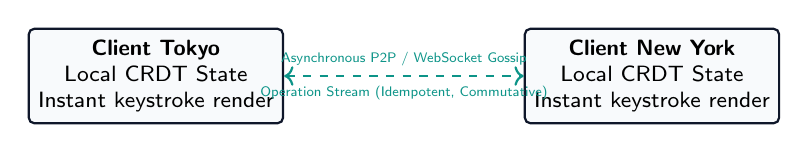
\begin{tikzpicture}[
  scale=0.9,
  user/.style={rectangle, draw=headingblue, fill=codebg, thick, rounded corners=2pt, minimum width=3.2cm, minimum height=1.2cm, align=center, font=\sffamily\footnotesize},
  sync/.style={<->, thick, dashed, color=intuitionTeal}
]
  \node[user] (u1) at (0, 0) {\textbf{Client Tokyo}\\Local CRDT State\\Instant keystroke render};
  \node[user] (u2) at (7, 0) {\textbf{Client New York}\\Local CRDT State\\Instant keystroke render};

  \draw[sync] (u1) -- node[above, font=\sffamily\tiny] {Asynchronous P2P / WebSocket Gossip} node[below, font=\sffamily\tiny] {Operation Stream (Idempotent, Commutative)} (u2);
\end{tikzpicture}
\end{figure}

1. \textbf{Local Optimistic Execution}: Use a sequence CRDT (such as Yjs or Automerge based on RGA---Replicated Growable Array). Every character insertion creates an element with a globally unique, fractional ID: $(\text{LamportTS}, \text{ClientID}, \text{Offset})$. Characters are rendered to the user's screen in $0\text{ ms}$.
2. \textbf{Asynchronous Commutative Merging}: Edit operations are broadcast over WebSockets asynchronously. Because CRDT operations form a join-semilattice (associative, commutative, and idempotent), operations can arrive out of order, be duplicated, or be delayed by hours without corrupting the document.
3. \textbf{Convergence}: When the network synchronizes, both Tokyo and New York mathematically converge to the exact same document string without locking or central coordinator intervention.

\section{Further Reading \& Citations}
\begin{itemize}[leftmargin=18pt]
  \item Gilbert, S., \& Lynch, N. (2002). \emph{Brewer's conjecture and the feasibility of consistent, available, partition-tolerant web services}. ACM SIGACT News, 33(2), 51--59.
  \item Abadi, D. J. (2012). \emph{Consistency tradeoffs in modern distributed database system design: CAP is only part of the story}. Computer, 45(2), 37--42.
  \item Ongaro, D., \& Ousterhout, J. (2014). \emph{In search of an understandable consensus algorithm}. In USENIX Annual Technical Conference (ATC 14), 305--319.
  \item Mahajan, P., Alvisi, L., \& Dahlin, M. (2011). \emph{Consistency, availability, and convergence}. UT Austin Technical Report TR-11-22.
\end{itemize}

\chapter{Transactions and Concurrency}
\label{ch:transactions-concurrency}

\begin{chaptergoalsbox}
\textbf{What you will learn:}
\begin{itemize}[leftmargin=12pt]
  \item The fundamental atomicity problem across autonomous nodes: why single-node ACID fails across network boundaries.
  \item The Two-Phase Commit (2PC) protocol: Prepare phase, Commit phase, and failure state machines.
  \item Coordinator crash modes, in-doubt participants, blocking hazards, and catastrophic single-point-of-failure locks.
  \item The Three-Phase Commit (3PC) protocol: PreCommit phase, non-blocking guarantees, and network partition limitations.
  \item Distributed deadlocks: wait-for graphs, cycle detection, Wound-Wait vs. Wait-Die deadlock prevention algorithms.
\end{itemize}

\textbf{What you should already understand:}
\begin{itemize}[leftmargin=12pt]
  \item Relational database transactions: ACID properties, write-ahead logging (WAL), two-phase locking (2PL).
  \item Consensus algorithms (Raft) and quorum rules from Chapter~\ref{ch:cap-consistency}.
\end{itemize}

\textbf{Why this topic exists:}
Enterprise systems must frequently coordinate state mutations across distinct, physically separated databases---such as deducting funds from an Oracle ledger and crediting loyalty points in a PostgreSQL cluster. Without atomic commit protocols, partial network failures leave balances permanently desynchronized.

\textbf{Motivating practical problem:}
A banking platform initiates an account transfer across two sharded databases. Database A successfully deducts \$10,000 from the sender. The application server coordinating the transfer crashes from an out-of-memory killer before sending the commit command to Database B. The sender's money is gone, the recipient never receives it, and the database locks on both accounts remain frozen indefinitely.
\end{chaptergoalsbox}

\section{The Distributed Atomicity Challenge}

On a single relational database engine, atomicity is guaranteed by an append-only Write-Ahead Log (WAL) managed by a central recovery engine. When a transaction commits, the engine writes a single \texttt{COMMIT} record to disk and calls \texttt{fsync()}. If the machine crashes before this record hits disk, recovery rolls back the uncommitted changes; if it crashes after, recovery rolls forward.

In a distributed system, a single logical transaction touches multiple independent databases (cohorts or participants) hosted on different servers. No single physical disk exists to host a shared WAL commit record. If participant $A$ commits its local transaction and participant $B$ crashes during its commit, the distributed transaction violates Atomicity: some changes persist while others vanish.

\section{The Two-Phase Commit (2PC) Protocol}

Two-Phase Commit, formalized by Jim Gray in 1978, is the foundational atomic commit protocol designed to ensure that all participants either commit or abort together, regardless of individual node crashes.

\subsection{Protocol Flow}

The protocol coordinates one \textbf{Coordinator} and $N$ \textbf{Participants} across two distinct phases:

\begin{figure}[htbp]
\centering
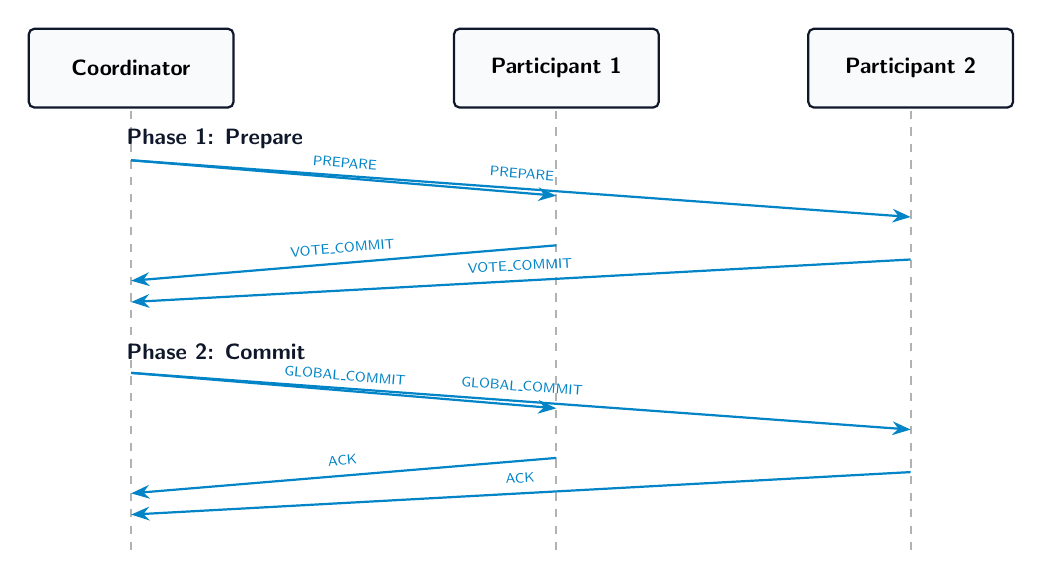
\begin{tikzpicture}[
  scale=0.9,
  node distance=2.5cm,
  entity/.style={rectangle, draw=headingblue, fill=codebg, thick, rounded corners=2pt, minimum width=2.6cm, minimum height=1.0cm, align=center, font=\sffamily\footnotesize},
  timeline/.style={thick, dashed, color=gray!60},
  msg/.style={-{Stealth[scale=1.0]}, thick, color=linkblue}
]
  \node[entity] (coord) at (0, 0) {\textbf{Coordinator}};
  \node[entity] (p1) at (6, 0) {\textbf{Participant 1}};
  \node[entity] (p2) at (11, 0) {\textbf{Participant 2}};

  \draw[timeline] (0, -0.6) -- (0, -6.8);
  \draw[timeline] (6, -0.6) -- (6, -6.8);
  \draw[timeline] (11, -0.6) -- (11, -6.8);

  % Phase 1
  \node[anchor=west, font=\sffamily\bfseries\footnotesize, color=headingblue] at (-0.2, -1.0) {Phase 1: Prepare};
  \draw[msg] (0, -1.3) -- node[above, sloped, font=\sffamily\tiny] {PREPARE} (6, -1.8);
  \draw[msg] (0, -1.3) -- node[above, sloped, font=\sffamily\tiny] {PREPARE} (11, -2.1);

  \draw[msg] (6, -2.5) -- node[above, sloped, font=\sffamily\tiny] {VOTE\_COMMIT} (0, -3.0);
  \draw[msg] (11, -2.7) -- node[above, sloped, font=\sffamily\tiny] {VOTE\_COMMIT} (0, -3.3);

  % Phase 2
  \node[anchor=west, font=\sffamily\bfseries\footnotesize, color=headingblue] at (-0.2, -4.0) {Phase 2: Commit};
  \draw[msg] (0, -4.3) -- node[above, sloped, font=\sffamily\tiny] {GLOBAL\_COMMIT} (6, -4.8);
  \draw[msg] (0, -4.3) -- node[above, sloped, font=\sffamily\tiny] {GLOBAL\_COMMIT} (11, -5.1);

  \draw[msg] (6, -5.5) -- node[above, sloped, font=\sffamily\tiny] {ACK} (0, -6.0);
  \draw[msg] (11, -5.7) -- node[above, sloped, font=\sffamily\tiny] {ACK} (0, -6.3);
\end{tikzpicture}
\caption{Two-Phase Commit (2PC) Protocol Sequence with Successful Agreement}
\label{fig:2pc-sequence}
\end{figure}

\begin{enumerate}[leftmargin=18pt]
  \item \textbf{Phase 1: Prepare (Voting Phase)}
  \begin{itemize}[leftmargin=12pt]
    \item The coordinator assigns a globally unique transaction ID ($TxID$) and sends a \texttt{PREPARE} message to all participants.
    \item Each participant executes the transaction locally: acquires row-level locks, writes mutations and undo logs to disk, but \textbf{does not commit}.
    \item If the participant successfully prepares and guarantees it can commit even if it crashes and reboots, it logs a \texttt{PREPARED} record to its local WAL and replies with \texttt{VOTE\_COMMIT}.
    \item If the participant fails to acquire locks, encounters a constraint violation, or runs out of disk space, it writes an \texttt{ABORT} record and replies with \texttt{VOTE\_ABORT}.
  \end{itemize}
  \item \textbf{Phase 2: Commit (Decision Phase)}
  \begin{itemize}[leftmargin=12pt]
    \item If \textbf{all} participants voted \texttt{VOTE\_COMMIT}, the coordinator writes a \texttt{GLOBAL\_COMMIT} record to its local WAL and broadcasts \texttt{GLOBAL\_COMMIT} to all participants.
    \item If \textbf{any} participant voted \texttt{VOTE\_ABORT} (or timed out without responding), the coordinator writes a \texttt{GLOBAL\_ABORT} record to its WAL and broadcasts \texttt{GLOBAL\_ABORT}.
    \item Participants receive the decision, apply or rollback the changes, release all held locks, and reply with an \texttt{ACK}.
    \item Once all ACKs are collected, the coordinator writes an \texttt{END} record to its log.
  \end{itemize}
\end{enumerate}

\subsection{The Blocking Problem: In-Doubt Participants}

The fatal vulnerability of 2PC is that it is a \textbf{blocking protocol}. If the coordinator crashes after participants have voted to commit but before delivering the final decision, participants enter an \textbf{in-doubt} state.

\begin{productionwarningbox}[The Catastrophic Blocking State of 2PC]
Consider the scenario where Participant 1 votes \texttt{VOTE\_COMMIT}. At that instant, Participant 1 surrenders autonomous control over its local resources:
\begin{itemize}[leftmargin=12pt]
  \item It \textbf{cannot unilaterally abort}, because the coordinator may have received all votes and sent \texttt{GLOBAL\_COMMIT} to Participant 2 before crashing. Unilateral abort would violate Atomicity.
  \item It \textbf{cannot unilaterally commit}, because Participant 2 might have voted \texttt{VOTE\_ABORT}, prompting the coordinator to decide abort. Unilateral commit would violate Atomicity.
\end{itemize}
Therefore, Participant 1 \textbf{must block indefinitely}, holding all row locks and preventing other transactions from accessing those rows until the coordinator recovers its WAL from disk! In cloud production environments, an in-doubt blocking state can lock tables for hours, cascading into thread pool exhaustion and complete platform outages.
\end{productionwarningbox}

\begin{lstlisting}[language=Python, caption={Python Demonstration of 2PC Participant Recovery Machine}]
import enum

class State(enum.Enum):
    INIT = 1
    PREPARED = 2
    COMMITTED = 3
    ABORTED = 4

class Participant2PC:
    def __init__(self, node_id: str):
        self.node_id = node_id
        self.state = State.INIT
        self.wal_log = []

    def on_receive_prepare(self, tx_id: str) -> bool:
        # Step 1: Check constraints, acquire locks, write undo/redo log to disk
        can_commit = self._acquire_locks_and_reserve(tx_id)
        if can_commit:
            self._write_wal(tx_id, "PREPARED")
            self.state = State.PREPARED
            return True # VOTE_COMMIT
        else:
            self._write_wal(tx_id, "ABORTED")
            self.state = State.ABORTED
            self._release_locks(tx_id)
            return False # VOTE_ABORT

    def on_receive_decision(self, tx_id: str, decision: str):
        if decision == "GLOBAL_COMMIT":
            self._write_wal(tx_id, "COMMITTED")
            self._finalize_commit(tx_id)
            self.state = State.COMMITTED
        else:
            self._write_wal(tx_id, "ABORTED")
            self._rollback(tx_id)
            self.state = State.ABORTED
        self._release_locks(tx_id)

    def recover_from_crash(self, tx_id: str):
        """Executed upon node reboot by scanning local WAL."""
        last_log = self._read_last_wal(tx_id)
        if last_log == "COMMITTED":
            self._finalize_commit(tx_id)
        elif last_log == "ABORTED" or last_log is None:
            self._rollback(tx_id)
        elif last_log == "PREPARED":
            # CRITICAL: We are IN-DOUBT!
            # We cannot resolve independently. Must query coordinator or peers.
            self._enter_blocking_in_doubt_state(tx_id)
\end{lstlisting}

\section{Three-Phase Commit (3PC)}

In 1981, Dale Skeen developed the Three-Phase Commit (3PC) protocol to eliminate the blocking hazard of 2PC. 3PC introduces an intermediate state---\textbf{PreCommit}---and assumes a \textbf{synchronous network model} with a bounded failure detector.

\subsection{Protocol Stages}

\begin{enumerate}[leftmargin=18pt]
  \item \textbf{Phase 1: Can-Commit?}: Coordinator queries participants. If all vote Yes, proceed.
  \item \textbf{Phase 2: Pre-Commit}: Coordinator issues \texttt{PRECOMMIT}. Participants enter the \texttt{PreCommit} state and acknowledge. Entering \texttt{PreCommit} guarantees that all participants voted Yes, and that no node will abort.
  \item \textbf{Phase 3: Do-Commit}: Coordinator issues \texttt{DO\_COMMIT}. All participants finalize their writes.
\end{enumerate}

\begin{figure}[htbp]
\centering
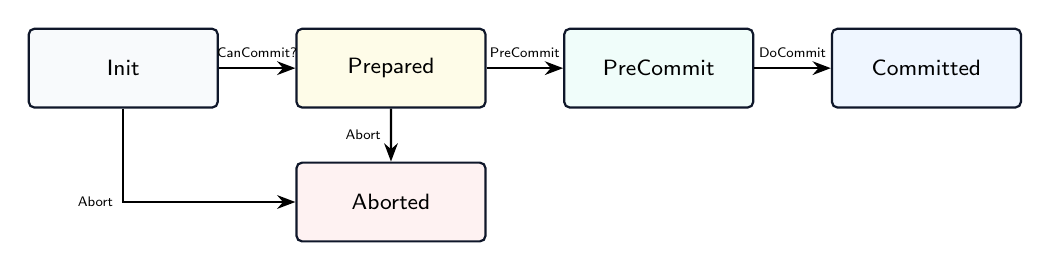
\begin{tikzpicture}[
  scale=0.85,
  state/.style={rectangle, draw=headingblue, fill=codebg, thick, rounded corners=2pt, minimum width=2.4cm, minimum height=1.0cm, align=center, font=\sffamily\footnotesize}
]
  \node[state] (init) at (0, 0) {Init};
  \node[state, fill=mistakeBg] (prep) at (4, 0) {Prepared};
  \node[state, fill=intuitionBg] (precommit) at (8, 0) {PreCommit};
  \node[state, fill=exampleBg] (commit) at (12, 0) {Committed};
  \node[state, fill=warningBg] (abort) at (4, -2) {Aborted};

  \draw[-{Stealth[scale=1.0]}, thick] (init) -- node[above, font=\sffamily\tiny] {CanCommit?} (prep);
  \draw[-{Stealth[scale=1.0]}, thick] (prep) -- node[above, font=\sffamily\tiny] {PreCommit} (precommit);
  \draw[-{Stealth[scale=1.0]}, thick] (precommit) -- node[above, font=\sffamily\tiny] {DoCommit} (commit);
  \draw[-{Stealth[scale=1.0]}, thick] (init) |- node[left, font=\sffamily\tiny] {Abort} (abort);
  \draw[-{Stealth[scale=1.0]}, thick] (prep) -- node[left, font=\sffamily\tiny] {Abort} (abort);
\end{tikzpicture}
\caption{State Transitions of a Participant in Three-Phase Commit (3PC)}
\label{fig:3pc-states}
\end{figure}

\subsection{Why 3PC is Rarely Used in Production}

Although 3PC eliminates blocking under a fail-stop model in synchronous networks, it fails completely under real-world \textbf{network partitions}:
\begin{itemize}[leftmargin=18pt]
  \item If a network partition splits the cluster during the PreCommit phase, nodes on one side of the partition timeout and abort, while nodes on the other side advance from PreCommit to Commit.
  \item This creates split-brain state corruption, violating Distributed Atomicity.
\end{itemize}
Because real networks are asynchronous and subject to partitions, modern distributed engines (CockroachDB, TiDB, YugabyteDB) reject 3PC. Instead, they implement \textbf{Two-Phase Commit layered on top of Raft or Paxos}: the 2PC transaction coordinator and transaction logs are themselves replicated state machines, guaranteeing that coordinator failure can never cause permanent blocking.

\section{Distributed Deadlocks and Prevention}

When transactions execute across multiple distributed nodes and acquire row-level locks incrementally (Two-Phase Locking, 2PL), circular wait conditions inevitably occur.

\begin{figure}[htbp]
\centering
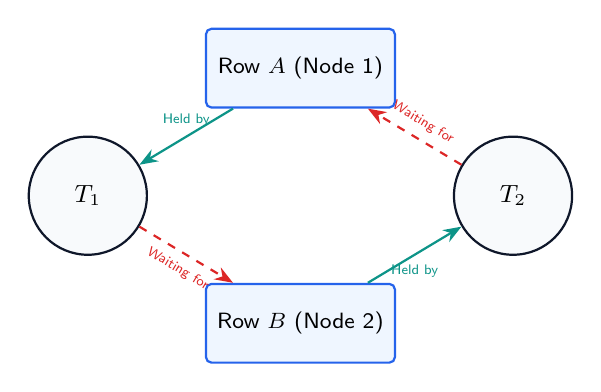
\begin{tikzpicture}[
  scale=0.9,
  tx/.style={circle, draw=headingblue, fill=codebg, thick, minimum size=1.5cm, align=center, font=\sffamily\small},
  res/.style={rectangle, draw=exampleBlue, fill=exampleBg, thick, rounded corners=2pt, minimum width=2.4cm, minimum height=1.0cm, align=center, font=\sffamily\footnotesize}
]
  \node[tx] (t1) at (0, 0) {$T_1$};
  \node[tx] (t2) at (6, 0) {$T_2$};
  \node[res] (r1) at (3, 1.8) {Row $A$ (Node 1)};
  \node[res] (r2) at (3, -1.8) {Row $B$ (Node 2)};

  \draw[-{Stealth[scale=1.0]}, thick, color=intuitionTeal] (r1) -- node[above, font=\sffamily\tiny] {Held by} (t1);
  \draw[-{Stealth[scale=1.0]}, thick, dashed, color=warningRed] (t1) -- node[below, sloped, font=\sffamily\tiny] {Waiting for} (r2);

  \draw[-{Stealth[scale=1.0]}, thick, color=intuitionTeal] (r2) -- node[below, font=\sffamily\tiny] {Held by} (t2);
  \draw[-{Stealth[scale=1.0]}, thick, dashed, color=warningRed] (t2) -- node[above, sloped, font=\sffamily\tiny] {Waiting for} (r1);
\end{tikzpicture}
\caption{Distributed Deadlock Cycle: Transactions $T_1$ and $T_2$ Waiting across Physical Nodes}
\label{fig:distributed-deadlock}
\end{figure}

\subsection{Wait-For Graphs and Centralized Detection}

In centralized databases, the engine maintains an in-memory Wait-For Graph (WFG) where directed edges represent $T_i \to T_j$ ($T_i$ is waiting for a lock held by $T_j$). Deadlocks are detected by executing Tarjan's strongly connected components algorithm or cycle detection on the graph.

In distributed systems, constructing a global WFG requires all nodes to transmit local lock wait events to a central deadlock detector service. Network transit delays cause \textbf{phantom deadlocks}: the detector observes a cycle based on delayed messages, even though one of the transactions has already released its lock and committed.

\subsection{Deadlock Prevention: Wait-Die vs. Wound-Wait}

To eliminate deadlock cycles without distributed graph traversal, systems assign each transaction a monotonically increasing, unique logical timestamp $TS(T)$ when the transaction begins. The older transaction has a smaller numerical timestamp ($TS(T_{\text{old}}) < TS(T_{\text{young}})$).

Suppose transaction $T_i$ requests a lock currently held by transaction $T_j$:

\begin{table}[htbp]
\centering\small
\begin{tabular}{lp{5.8cm}p{5.8cm}}
\toprule
\textbf{Algorithm} & \textbf{When $T_i$ is Older ($TS(T_i) < TS(T_j)$)} & \textbf{When $T_i$ is Younger ($TS(T_i) > TS(T_j)$)} \\
\midrule
\textbf{Wait-Die} & \textbf{Wait}: $T_i$ is permitted to wait for the younger $T_j$. & \textbf{Die}: $T_i$ dies (aborts and restarts with its original timestamp). \\
\textbf{Wound-Wait} & \textbf{Wound}: $T_i$ preempts $T_j$. $T_j$ is wounded (aborts and releases its locks). & \textbf{Wait}: $T_i$ is permitted to wait for the older $T_j$. \\
\bottomrule
\end{tabular}
\caption{Comparison of Wait-Die and Wound-Wait Deadlock Prevention Protocols}
\label{tab:deadlock-algorithms}
\end{table}

\begin{underthehoodbox}[Why Wound-Wait Minimizes Cascading Aborts]
In \textbf{Wait-Die}, an older transaction waits for younger ones. As a transaction ages, it is forced to wait more frequently, and younger transactions continually die and restart, leading to high abort rates and wasted work.
In \textbf{Wound-Wait}, an older transaction immediately ``wounds'' (preempts) any younger transaction blocking its path. Younger transactions only wait for older ones; they never block an older transaction. Consequently, as a transaction gets older, it accumulates priority and clears its own path without ever being aborted. When a wounded transaction restarts, it retains its original timestamp, guaranteeing it will eventually become the oldest transaction and finish without starvation.
\end{underthehoodbox}

\section{Summary \& Key Takeaways}
\begin{itemize}[leftmargin=18pt]
  \item Single-node ACID cannot guarantee cross-network atomicity; distributed transactions require atomic commit protocols.
  \item Two-Phase Commit (2PC) separates execution into Prepare and Commit phases, requiring unanimous agreement before writing a global commit.
  \item 2PC is fundamentally vulnerable to coordinator crashes: participants that vote to commit enter an \textbf{in-doubt} blocking state and cannot unilaterally resolve locks without risking state corruption.
  \item Three-Phase Commit (3PC) eliminates blocking in synchronous networks by introducing a PreCommit phase, but partitions cause split-brain data corruption.
  \item Modern distributed engines solve 2PC blocking by replicating the coordinator and transaction logs via Raft or Paxos quorums.
  \item Distributed deadlocks can be prevented without global wait-for graph cycle detection using timestamp-ordered non-preemptive (\textbf{Wait-Die}) or preemptive (\textbf{Wound-Wait}) algorithms.
\end{itemize}

\section{Exercises}

\subsection{Mechanics}
Trace a 2PC execution involving Coordinator $C$ and three participants $P_1, P_2, P_3$:
\begin{enumerate}[leftmargin=18pt]
  \item $P_1$ and $P_2$ vote \texttt{VOTE\_COMMIT}. $P_3$ experiences a unique key violation and votes \texttt{VOTE\_ABORT}.
  \item Detail the exact messages sent by the coordinator in Phase 2, the disk operations executed by $P_1$ and $P_2$, and the final state of all participants.
\end{enumerate}

\subsection{Debugging}
An engineer analyzes a thread dump from a microservice deployment utilizing Java Transaction API (JTA) with XA two-phase commit over two PostgreSQL databases. All 200 HTTP worker threads are blocked waiting for database connections. The database connection pools are 100\% saturated. Querying \texttt{pg\_prepared\_xacts} reveals 15 transactions in the \texttt{prepared} state dating back 14 hours. Explain why the connection pool is exhausted and detail the query to safely unlock the database.

\subsection{Architecture}
CockroachDB executes distributed multi-shard ACID transactions without a centralized 2PC coordinator. Explain how CockroachDB implements 2PC using \textbf{Transaction Records} stored as normal keys in a Raft range, \textbf{Write Intents}, and \textbf{Wound-Wait} concurrency control.

\section{Detailed Solutions}

\subsection{Solution to Mechanics Exercise}
\begin{enumerate}[leftmargin=18pt]
  \item Coordinator $C$ collects votes: $P_1 \to \texttt{COMMIT}$, $P_2 \to \texttt{COMMIT}$, $P_3 \to \texttt{ABORT}$.
  \item Because unanimous consent is required, the coordinator chooses \textbf{Abort}.
  \item $C$ writes \texttt{GLOBAL\_ABORT} to its local WAL and flushes to disk.
  \item $C$ broadcasts \texttt{GLOBAL\_ABORT} to $P_1, P_2, P_3$.
  \item $P_1$ and $P_2$ receive \texttt{GLOBAL\_ABORT}: they parse their local undo logs, rollback all mutated rows to their pre-transaction values, write an \texttt{ABORTED} record to their local WAL, release all held locks on disk/RAM, and reply with \texttt{ACK}.
  \item $P_3$ receives \texttt{GLOBAL\_ABORT}, writes an \texttt{ABORTED} log, and replies with \texttt{ACK}.
  \item $C$ collects all ACKs and writes \texttt{END} to its WAL. All nodes finish in the \textbf{Aborted} state; Atomicity is preserved.
\end{enumerate}

\subsection{Solution to Debugging Exercise}
\textbf{Root Cause:} The application server acting as the XA Transaction Manager crashed (or suffered a network split) after issuing \texttt{PREPARE TRANSACTION} to PostgreSQL, but before issuing \texttt{COMMIT PREPARED} or \texttt{ROLLBACK PREPARED}. In PostgreSQL, a prepared transaction survives client disconnects and server restarts. It holds its acquired row and table locks indefinitely until explicitly resolved. Any incoming web request attempting to update those same rows is blocked, exhausting the application connection pool.
\textbf{Resolution Query:}
To inspect the orphaned in-doubt transactions:
\begin{lstlisting}[language=SQL]
SELECT gid, prepared, owner, database FROM pg_prepared_xacts;
\end{lstlisting}
To manually rollback the stuck transaction and release all row locks:
\begin{lstlisting}[language=SQL]
ROLLBACK PREPARED 'tx_gid_string_from_above';
\end{lstlisting}

\subsection{Solution to Architecture Exercise}
\textbf{CockroachDB's Distributed Transaction Architecture:}
\begin{enumerate}[leftmargin=18pt]
  \item \textbf{Transaction Record}: When a client initiates a transaction, it creates a Transaction Record in the Raft range containing the transaction's primary key. The record has states: \texttt{PENDING}, \texttt{STAGING}, \texttt{COMMITTED}, or \texttt{ABORTED}. Because this record is replicated via Raft, it cannot be lost to single-node crashes.
  \item \textbf{Write Intents}: When the transaction updates rows across other ranges (secondary keys), it writes an inline marker called a \emph{Write Intent}. A Write Intent points to the Transaction Record and contains the uncommitted value alongside an in-memory lock.
  \item \textbf{Concurrency via Wound-Wait}: If transaction $T_{\text{young}}$ encounters a Write Intent written by $T_{\text{old}}$, $T_{\text{young}}$ waits. If $T_{\text{old}}$ encounters a Write Intent written by $T_{\text{young}}$, $T_{\text{old}}$ wounds $T_{\text{young}}$ by setting $T_{\text{young}}$'s Transaction Record to \texttt{ABORTED}.
  \item \textbf{Atomic Commit Point}: The entire distributed transaction commits atomically the exact instant the primary Transaction Record transitions from \texttt{PENDING} to \texttt{COMMITTED} in Raft. Asynchronously, the coordinator resolves the Write Intents into permanent MVCC records. If another client reads a Write Intent before resolution, it inspects the primary Transaction Record to determine whether to return the new or old value.
\end{enumerate}

\section{Further Reading \& Citations}
\begin{itemize}[leftmargin=18pt]
  \item Gray, J. (1978). \emph{Notes on data base operating systems}. Operating Systems, An Advanced Course, Springer-Verlag, 393--481.
  \item Skeen, D. (1981). \emph{Nonblocking commit protocols}. In Proceedings of the 1981 ACM SIGMOD international conference on Management of data, 133--142.
  \item Rosenkrantz, D. J., Stearns, R. E., \& Lewis, P. M. (1978). \emph{System level concurrency control for distributed database systems}. ACM Transactions on Database Systems (TODS), 3(2), 178--198.
  \item Bernstein, P. A., Hadzilacos, V., \& Goodman, N. (1987). \emph{Concurrency control and recovery in database systems}. Addison-Wesley.
\end{itemize}

\chapter{Messaging Systems and Asynchronous Pipelines}
\label{ch:messaging-systems}

\begin{chaptergoalsbox}
\textbf{What you will learn:}
\begin{itemize}[leftmargin=12pt]
  \item Core messaging patterns: Point-to-Point queues vs. Publish-Subscribe (Pub/Sub) event streams.
  \item Delivery semantics: At-most-once, At-least-once, and Exactly-once processing (deduplication windows and idempotent consumers).
  \item Competing consumers, backpressure, prefetch buffers, and flow control.
  \item Poison messages, retry topologies, and Dead Letter Queues (DLQs).
  \item Idempotency keys, out-of-order message handling, and tombstone markers.
\end{itemize}

\textbf{What you should already understand:}
\begin{itemize}[leftmargin=12pt]
  \item TCP sockets, HTTP REST interfaces, and asynchronous job queues.
  \item Relational transaction concepts and data persistence from Volume I.
\end{itemize}

\textbf{Why this topic exists:}
Synchronous HTTP/gRPC RPC calls introduce tight temporal and spatial coupling: if the downstream service is down or experiencing high latency, the upstream caller blocks, saturating connection pools and cascading into catastrophic cluster-wide failure. Asynchronous messaging decouples producers and consumers in both time and space.

\textbf{Motivating practical problem:}
A payment processing pipeline uses an asynchronous queue to charge customer credit cards. During a transient database timeout, the queue re-delivers 10,000 unacknowledged messages. Because the consumer lacks idempotency guards, 4,200 customers are charged double, causing massive credit card dispute chargeback fees and merchant account suspension.
\end{chaptergoalsbox}

\section{Queues vs. Streams: Structural Trade-Offs}

Distributed message passing architectures generally fall into two distinct paradigms: message queues and event streams.

\begin{figure}[htbp]
\centering
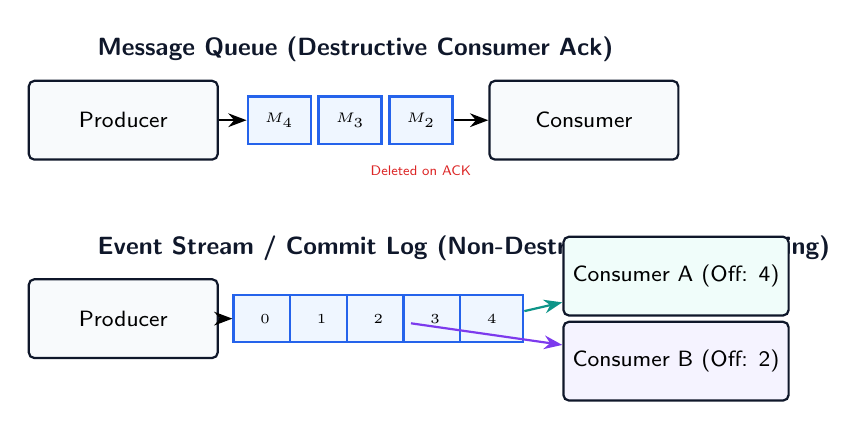
\begin{tikzpicture}[
  scale=0.9,
  box/.style={rectangle, draw=headingblue, fill=codebg, thick, rounded corners=2pt, minimum width=2.4cm, minimum height=1.0cm, align=center, font=\sffamily\footnotesize},
  elem/.style={rectangle, draw=exampleBlue, fill=exampleBg, thick, minimum width=0.8cm, minimum height=0.6cm, font=\sffamily\tiny}
]
  % Queue diagram
  \node[anchor=west, font=\sffamily\bfseries\small, color=headingblue] at (-0.5, 2.2) {Message Queue (Destructive Consumer Ack)};
  \node[box] (p1) at (0, 1.2) {Producer};
  \node[elem] (m1) at (2.2, 1.2) {$M_4$};
  \node[elem] (m2) at (3.2, 1.2) {$M_3$};
  \node[elem] (m3) at (4.2, 1.2) {$M_2$};
  \node[box] (c1) at (6.5, 1.2) {Consumer};
  \draw[-{Stealth[scale=1.0]}, thick] (p1) -- (m1);
  \draw[-{Stealth[scale=1.0]}, thick] (m3) -- (c1);
  \node[anchor=north, font=\sffamily\tiny, color=warningRed] at (4.2, 0.7) {Deleted on ACK};

  % Log diagram
  \node[anchor=west, font=\sffamily\bfseries\small, color=headingblue] at (-0.5, -0.6) {Event Stream / Commit Log (Non-Destructive Offset Tracking)};
  \node[box] (p2) at (0, -1.6) {Producer};
  \node[elem] (e0) at (2.0, -1.6) {$0$};
  \node[elem] (e1) at (2.8, -1.6) {$1$};
  \node[elem] (e2) at (3.6, -1.6) {$2$};
  \node[elem] (e3) at (4.4, -1.6) {$3$};
  \node[elem] (e4) at (5.2, -1.6) {$4$};

  \node[box, fill=intuitionBg] (c_a) at (7.8, -1.0) {Consumer A (Off: 4)};
  \node[box, fill=tryBg] (c_b) at (7.8, -2.2) {Consumer B (Off: 2)};

  \draw[-{Stealth[scale=1.0]}, thick] (p2) -- (e0);
  \draw[-{Stealth[scale=1.0]}, thick, color=intuitionTeal] (e4) -- (c_a);
  \draw[-{Stealth[scale=1.0]}, thick, color=tryViolet] (e2) -- (c_b);
\end{tikzpicture}
\caption{Comparison of Traditional Message Queues vs. Persistent Log Streams}
\label{fig:queue-vs-stream}
\end{figure}

\begin{table}[htbp]
\centering\small
\begin{tabular}{lp{5.5cm}p{5.5cm}}
\toprule
\textbf{Dimension} & \textbf{Traditional Message Queue (RabbitMQ, SQS)} & \textbf{Event Stream / Append Log (Kafka, Pulsar)} \\
\midrule
\textbf{State Retention} & Transient. Messages are deleted immediately upon successful consumer acknowledgment. & Persistent. Immutable append-only log retained by time (retention hours) or size. \\
\textbf{Consumer Scalability} & Competing consumers pull from a single shared queue; work is distributed dynamically. & Partition-bound. Maximum parallel consumers in a group equals the number of partitions. \\
\textbf{Replayability} & Impossible. Once acknowledged, the message ceases to exist. & Native. Any consumer can reset its offset backwards to replay historical days of data. \\
\textbf{Ordering} & Total FIFO across a single queue, but broken when competing consumers fail and requeue. & Strict per-partition ordering guaranteed indefinitely. \\
\bottomrule
\end{tabular}
\caption{Architectural Comparison: Queues vs. Streams}
\label{tab:queue-vs-stream}
\end{table}

\section{Message Delivery Semantics}

In an ideal theoretical world, systems would deliver every message exactly once, with zero loss, zero duplication, and zero delay. Across real physical networks, packet losses and timeout retransmissions create distinct delivery semantics:

\subsection{At-Most-Once Delivery}
\begin{itemize}[leftmargin=18pt]
  \item \textbf{Mechanics}: The consumer receives the message, advances its offset or sends an acknowledgment to the broker \textbf{before} processing the message.
  \item \textbf{Failure Mode}: If the consumer crashes during processing, the broker believes the message was handled and never resends it. The message is permanently lost.
  \item \textbf{Use Case}: High-frequency metrics, sensor telemetry where occasional drops are preferable to blocking backpressure.
\end{itemize}

\subsection{At-Least-Once Delivery}
\begin{itemize}[leftmargin=18pt]
  \item \textbf{Mechanics}: The consumer receives the message, fully completes processing and persistence, and \textbf{then} sends an acknowledgment to the broker.
  \item \textbf{Failure Mode}: If the consumer crashes or network packets drop during the ACK transmission, the broker assumes the consumer died and re-delivers the message to another consumer. The message is processed more than once.
  \item \textbf{Production Reality}: This is the standard delivery mode of modern enterprise systems.
\end{itemize}

\subsection{The Myth and Reality of ``Exactly-Once''}

\begin{productionwarningbox}[The Network Impossibility of Physical Exactly-Once Delivery]
Physically delivering a message over an unreliable network exactly once is equivalent to solving the Two Generals' Problem, which is proven impossible. When brokers claim ``exactly-once semantics'' (EOS, such as Kafka's transactional API), they mean \textbf{effectively-once processing}:
\begin{equation}
\text{At-Least-Once Delivery} + \text{Idempotent Consumer / Deduplication} = \text{Effectively-Once Execution}
\end{equation}
If your downstream consumer executes a non-idempotent side effect (such as sending an SMS, dispatching an email, or calling a third-party non-transactional REST API), duplicates \textbf{will} trigger multiple side effects unless guarded by an application-level idempotency key.
\end{productionwarningbox}

\begin{figure}[htbp]
\centering
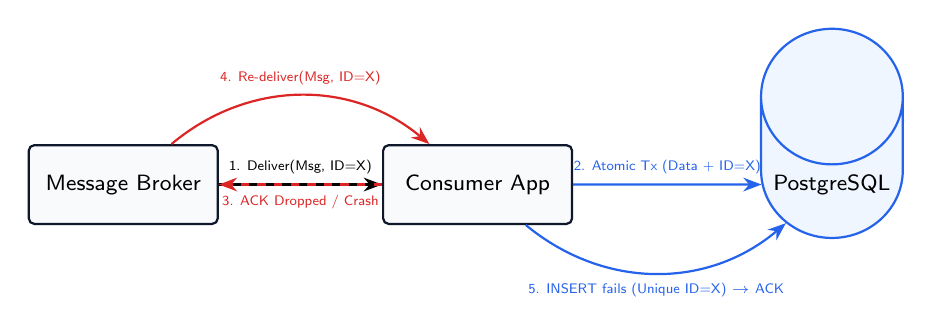
\begin{tikzpicture}[
  scale=0.9,
  client/.style={rectangle, draw=headingblue, fill=codebg, thick, rounded corners=2pt, minimum width=2.4cm, minimum height=1.0cm, align=center, font=\sffamily\footnotesize},
  db/.style={cylinder, draw=exampleBlue, fill=exampleBg, thick, shape border rotate=90, minimum width=1.8cm, minimum height=1.4cm, align=center, font=\sffamily\footnotesize}
]
  \node[client] (broker) at (0, 0) {Message Broker};
  \node[client] (consumer) at (5, 0) {Consumer App};
  \node[db] (db) at (10, 0) {PostgreSQL};

  \draw[-{Stealth[scale=1.0]}, thick] (broker) -- node[above, font=\sffamily\tiny] {1. Deliver(Msg, ID=X)} (consumer);
  \draw[-{Stealth[scale=1.0]}, thick, color=exampleBlue] (consumer) -- node[above, font=\sffamily\tiny] {2. Atomic Tx (Data + ID=X)} (db);
  \draw[-{Stealth[scale=1.0]}, thick, dashed, color=warningRed] (consumer) -- node[below, font=\sffamily\tiny] {3. ACK Dropped / Crash} (broker);
  \draw[-{Stealth[scale=1.0]}, thick, color=warningRed] (broker) to [bend left=40] node[above, font=\sffamily\tiny] {4. Re-deliver(Msg, ID=X)} (consumer);
  \draw[-{Stealth[scale=1.0]}, thick, color=exampleBlue] (consumer) to [bend right=40] node[below, font=\sffamily\tiny] {5. INSERT fails (Unique ID=X) $\to$ ACK} (db);
\end{tikzpicture}
\caption{Idempotent Consumer Deduplication via Database Unique Constraints}
\label{fig:idempotent-consumer}
\end{figure}

\begin{lstlisting}[language=Python, caption={Idempotent Consumer Implementation with Unique Key Deduplication}]
import psycopg2
from psycopg2 import IntegrityError

def process_order_message(conn, message: dict):
    """
    Guarantees exactly-once side-effect execution via atomic relational transaction.
    """
    message_id = message["id"]
    order_data = message["payload"]

    with conn.cursor() as cur:
        try:
            # 1. Attempt to insert message_id into processed_messages table
            cur.execute(
                "INSERT INTO processed_messages (message_id, processed_at) VALUES (%s, NOW());",
                (message_id,)
            )

            # 2. Execute business logic within the same transaction
            cur.execute(
                """
                INSERT INTO orders (order_id, customer_id, total_amount, status)
                VALUES (%s, %s, %s, %s);
                """,
                (order_data["order_id"], order_data["customer_id"], order_data["amount"], "CONFIRMED")
            )

            conn.commit()
            print(f"Successfully processed message {message_id}")

        except IntegrityError:
            # Duplicate message detected! Unique constraint on message_id violated.
            conn.rollback()
            print(f"Message {message_id} already processed. Safely ignoring and ACKing.")
\end{lstlisting}

\section{Poison Messages and Dead Letter Queues (DLQ)}

A \textbf{poison message} is a malformed or corrupted payload that causes a consumer to throw an unhandled exception every time it is read (e.g., invalid JSON syntax, null pointer, schema mismatch, or arithmetic overflow).

If a message broker automatically re-queues unacknowledged messages immediately upon consumer failure:
\begin{enumerate}[leftmargin=18pt]
  \item Consumer reads message $M$, crashes, and rejects $M$.
  \item Broker places $M$ back at the head of the queue.
  \item The same consumer (or a peer) immediately reads $M$ again and crashes.
  \item \textbf{Catastrophic Loop}: All consumers in the cluster enter an infinite crash loop, throughput drops to zero, and the CPU spikes to 100\% processing the same poison payload.
\end{enumerate}

\begin{figure}[htbp]
\centering
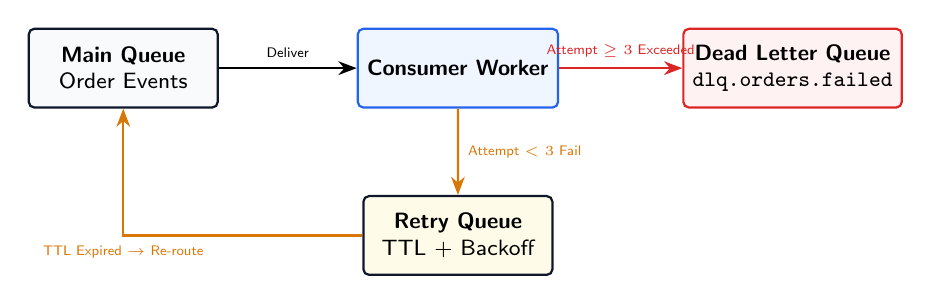
\begin{tikzpicture}[
  scale=0.85,
  q/.style={rectangle, draw=headingblue, fill=codebg, thick, rounded corners=2pt, minimum width=2.4cm, minimum height=1.0cm, align=center, font=\sffamily\footnotesize},
  c/.style={rectangle, draw=exampleBlue, fill=exampleBg, thick, rounded corners=2pt, minimum width=2.2cm, minimum height=1.0cm, align=center, font=\sffamily\footnotesize},
  dlq/.style={rectangle, draw=warningRed, fill=warningBg, thick, rounded corners=2pt, minimum width=2.4cm, minimum height=1.0cm, align=center, font=\sffamily\footnotesize}
]
  \node[q] (main) at (0, 0) {\textbf{Main Queue}\\Order Events};
  \node[c] (consumer) at (5, 0) {\textbf{Consumer Worker}};
  \node[q, fill=mistakeBg] (retry) at (5, -2.5) {\textbf{Retry Queue}\\TTL + Backoff};
  \node[dlq] (dlq) at (10, 0) {\textbf{Dead Letter Queue}\\\texttt{dlq.orders.failed}};

  \draw[-{Stealth[scale=1.0]}, thick] (main) -- node[above, font=\sffamily\tiny] {Deliver} (consumer);
  \draw[-{Stealth[scale=1.0]}, thick, color=mistakeAmber] (consumer) -- node[right, font=\sffamily\tiny] {Attempt $< 3$ Fail} (retry);
  \draw[-{Stealth[scale=1.0]}, thick, color=mistakeAmber] (retry) -| node[below, font=\sffamily\tiny] {TTL Expired $\to$ Re-route} (main);
  \draw[-{Stealth[scale=1.0]}, thick, color=warningRed] (consumer) -- node[above, font=\sffamily\tiny] {Attempt $\ge 3$ Exceeded} (dlq);
\end{tikzpicture}
\caption{Production Retry Pipeline with Dead Letter Queue (DLQ) Offloading}
\label{fig:dlq-pipeline}
\end{figure}

\begin{underthehoodbox}[Production Dead Letter Queue Invariants]
A robust messaging topology must adhere to three non-negotiable rules:
\begin{itemize}[leftmargin=12pt]
  \item \textbf{Bounded Retries}: Never retry infinitely. Set a hard cap (e.g., 3 to 5 attempts) tracked via an injected message header (\texttt{x-retry-count}).
  \item \textbf{Exponential Backoff with Jitter}: Never re-queue immediately. Route transient failures to delayed retry exchanges or dead-letter topics with exponential delays (e.g., $1\text{s}, 10\text{s}, 60\text{s}$) to give upstream services recovery windows.
  \item \textbf{DLQ Diagnostics \& Alerting}: When a message exhausts retries and enters the DLQ, preserve the original payload, the full stack trace, the offending worker host, and trigger a PagerDuty alert.
\end{itemize}
\end{underthehoodbox}

\section{Summary \& Key Takeaways}
\begin{itemize}[leftmargin=18pt]
  \item Message queues provide transient, destructive delivery for dynamic work distribution, whereas event streams provide immutable, ordered, replayable append logs.
  \item At-least-once delivery is the practical foundation of distributed messaging. Truly physical exactly-once delivery across networks is physically impossible due to the Two Generals' problem.
  \item Effectively-once processing requires pairing at-least-once delivery with \textbf{idempotent consumers} using unique idempotency keys and atomic database deduplication tables.
  \item Unhandled exceptions on malformed payloads create poison message infinite crash loops that can take down entire consumer clusters.
  \item Production pipelines isolate poison messages using bounded retry counters, delayed retry queues, and Dead Letter Queues (DLQs) with diagnostic telemetry.
\end{itemize}

\section{Exercises}

\subsection{Mechanics}
A payment service receives order charge events. Construct an idempotent SQL schema and an \texttt{UPSERT} query in PostgreSQL that safely handles repeated deliveries of payment authorization events without charging the customer twice.

\subsection{Debugging}
An operations team notices an alert: \emph{RabbitMQ Memory High Watermark Exceeded (Node Alarmed)}. Messages published to \texttt{order.events} are blocked. Investigation reveals that a consumer group has 10 workers, but the queue has 500,000 unacknowledged messages. The consumer configuration contains:
\begin{lstlisting}[language=Java]
channel.basicQos(0); // Prefetch count
\end{lstlisting}
Explain why RabbitMQ ran out of memory and why consumer workers stopped acknowledging messages.

\subsection{Architecture}
Design a distributed webhook notification delivery system (like Stripe's webhook infrastructure) capable of dispatching 50 million webhooks per day to arbitrary third-party customer endpoints. Address endpoint timeouts, unresponsive customer servers, exponential retry scheduling over 72 hours, and isolation so one slow customer cannot block other customers.

\section{Detailed Solutions}

\subsection{Solution to Mechanics Exercise}
\begin{lstlisting}[language=SQL]
-- Idempotent Ledger Schema
CREATE TABLE payment_authorizations (
    idempotency_key VARCHAR(64) PRIMARY KEY,
    customer_id VARCHAR(64) NOT NULL,
    amount_cents BIGINT NOT NULL,
    status VARCHAR(32) NOT NULL,
    created_at TIMESTAMPTZ NOT NULL DEFAULT NOW()
);

-- Safe Upsert Query: returns existing record on conflict without re-charging
INSERT INTO payment_authorizations (idempotency_key, customer_id, amount_cents, status)
VALUES ('pay_tok_948fbc', 'cust_123', 4999, 'AUTHORIZED')
ON CONFLICT (idempotency_key) DO UPDATE
SET status = payment_authorizations.status
RETURNING *;
\end{lstlisting}

\subsection{Solution to Debugging Exercise}
\textbf{The basicQos(0) Memory Trap:}
In AMQP / RabbitMQ, setting \texttt{basicQos(0)} specifies an \textbf{unlimited prefetch count}.
When workers connect and invoke \texttt{basicConsume}, RabbitMQ attempts to push \emph{every single message in the queue} across the TCP socket into the client workers' in-memory buffers as fast as the network allows.
Because the workers take time to process each message, hundreds of thousands of messages are pulled out of disk/broker management into unacknowledged RAM buffers.
The broker must track state metadata for all 500,000 in-flight unacknowledged deliveries in RAM. Once broker memory crosses the 40\% watermark, RabbitMQ triggers an alarm, suspends socket reading, and stops accepting new ACKs and publishes.
\textbf{The Fix:} Always set a bounded prefetch count:
\begin{lstlisting}[language=Java]
channel.basicQos(50); // Fetch at most 50 unacked messages per consumer thread
\end{lstlisting}

\subsection{Solution to Architecture Exercise}
\textbf{Distributed Webhook Dispatch Architecture:}
\begin{enumerate}[leftmargin=18pt]
  \item \textbf{Partitioning and Customer Isolation}: Route outgoing webhooks into tiered Kafka topics or partitioned queues based on customer hash: \texttt{webhooks.fast} and \texttt{webhooks.slow}. If customer $X$'s endpoint times out continuously, their events are dynamically downgraded to the slow tier, preventing thread starvation for healthy customers.
  \item \textbf{Tiered Delayed Retry Queues}:
  \begin{itemize}[leftmargin=12pt]
    \item Retry 1: 15 seconds delay.
    \item Retry 2: 5 minutes delay.
    \item Retry 3: 1 hour delay.
    \item Retry 4--10: Bounded exponential backoff up to 72 hours.
  \end{itemize}
  Implement delays using message timestamps and separate delayed topics (or Redis sorted sets where score is unix execution epoch).
  \item \textbf{HTTP Client Hard Limits}: Set strict timeouts on outbound connections: connect timeout $3\text{ s}$, read timeout $10\text{ s}$. Enforce circuit breakers per domain: if a customer domain fails 50 consecutive requests, short-circuit immediately.
\end{enumerate}

\section{Further Reading \& Citations}
\begin{itemize}[leftmargin=18pt]
  \item Kleppmann, M. (2017). \emph{Designing Data-Intensive Applications}. O'Reilly Media. Chapter 11: Stream Processing.
  \item Hohpe, G., \& Woolf, B. (2003). \emph{Enterprise Integration Patterns}. Addison-Wesley.
  \item Akidau, T., et al. (2015). \emph{The dataflow model: a practical approach to balancing correctness, latency, and cost in massive-scale, unbounded, out-of-order data processing}. Proceedings of the VLDB Endowment, 8(12), 1792--1803.
\end{itemize}

\chapter{Kafka and RabbitMQ Internals}
\label{ch:kafka-rabbitmq}

\begin{chaptergoalsbox}
\textbf{What you will learn:}
\begin{itemize}[leftmargin=12pt]
  \item Kernel I/O fundamentals from first principles: User Space vs. Kernel Space, OS Page Cache, and traditional \texttt{read()}/\texttt{write()} (4 copies) vs. \texttt{sendfile(2)} zero-copy.
  \item Apache Kafka storage and replication: segmented commit logs, sparse \texttt{.index} binary search, ISR, High Watermark (HW), and KRaft (\texttt{\_\_cluster\_metadata}).
  \item Kafka producer batching (\texttt{linger.ms}, \texttt{batch.size}, Kafka 3.0+ idempotent defaults) and consumer group rebalancing (\texttt{Range}, \texttt{RoundRobin}, \texttt{CooperativeSticky}).
  \item RabbitMQ AMQP 0-9-1 routing (Direct, Fanout, Topic, Headers exchanges), Erlang BEAM reductions, Mnesia metadata, and Quorum Queues vs. Classic Mirrored Queues.
\end{itemize}

\textbf{What you should already understand:}
\begin{itemize}[leftmargin=12pt]
  \item Raft majority quorums from Chapter~\ref{ch:cap-consistency} and queues vs. streams from Chapter~\ref{ch:messaging-systems}.
  \item No prior Linux kernel or Erlang background is assumed---we introduce page caches, system calls, and BEAM scheduling directly.
\end{itemize}

\textbf{Why this topic exists:}
Apache Kafka and RabbitMQ look similar on architecture slides---both move messages between services---but their internals are opposites. Treating them interchangeably leads to disaster: storing long-lived audit streams inside RabbitMQ RAM, or trying to route millions of per-user priority tasks through Kafka partitions.

\textbf{Motivating practical problem:}
A logistics platform uses RabbitMQ Classic Mirrored Queues to dispatch 40,000 shipment updates per second. When one broker reboots for security patching, resynchronizing mirrored queues locks the broker for four minutes and stalls checkout. After migrating to Kafka without understanding consumer rebalancing, deploying a new pod triggers a 90-second ``stop-the-world'' rebalance storm every time autoscaling runs.
\end{chaptergoalsbox}

\section{Kernel I/O Primer: Page Cache and Zero-Copy}

Before examining Kafka's disk format, we must answer a puzzle: how does Kafka sustain gigabytes per second of throughput when it writes every message to disk rather than keeping everything in application RAM? The secret lives inside the Linux operating system kernel.

\subsection{User Space, Kernel Space, and the OS Page Cache}

Modern CPUs enforce hardware privilege rings separating memory into two regions:
\begin{itemize}[leftmargin=18pt]
  \item \textbf{Kernel Space}: Privileged OS territory that owns hardware drivers (disks, network cards), TCP sockets, and the Virtual File System (VFS).
  \item \textbf{User Space}: Unprivileged memory where your Python, Java, or Go application runs. An application cannot touch a disk or network card directly; it must ask the kernel via a \textbf{system call} (such as \texttt{read()}, \texttt{write()}, or \texttt{sendfile()}), which pauses the thread and switches CPU mode into the kernel (a \textbf{context switch}).
\end{itemize}

Whenever the kernel reads or writes a file on disk, it automatically caches recently used $4\text{ KB}$ disk blocks inside free physical RAM called the \textbf{OS Page Cache}. Crucially, Kafka runs on the JVM, where caching millions of message objects inside Java heap memory wastes RAM on object headers and triggers long Stop-The-World garbage collection pauses. Instead, Kafka writes raw sequential bytes to files and lets the Linux Page Cache hold hot data in RAM with zero JVM GC overhead.

\subsection{Traditional \texttt{read()}/\texttt{write()} vs. \texttt{sendfile(2)} Zero-Copy}

Hardware controllers use \textbf{DMA (Direct Memory Access)} to transfer bytes between Disk/NIC and Kernel RAM without burning CPU cycles. Watch what happens when a traditional server reads a file from disk and sends it over a socket using standard \texttt{read()} followed by \texttt{write()} (Figure~\ref{fig:v4-ch05-zero-copy-comparison}, top):
\begin{enumerate}[leftmargin=18pt]
  \item \texttt{read()} context-switches to kernel; DMA copies bytes from Disk $\to$ OS Page Cache (Copy~1).
  \item CPU copies bytes from Page Cache $\to$ User-Space buffer (Copy~2); context-switches back to user space.
  \item \texttt{write()} context-switches to kernel; CPU copies bytes from User-Space buffer $\to$ Kernel Socket Buffer (Copy~3).
  \item Context-switches back to user space while DMA copies Socket Buffer $\to$ NIC (Copy~4).
\end{enumerate}
That costs \textbf{4 context switches and 4 data copies} (two of them wasting CPU) even though the broker never modified a single byte!

\begin{figure}[htbp]
\centering
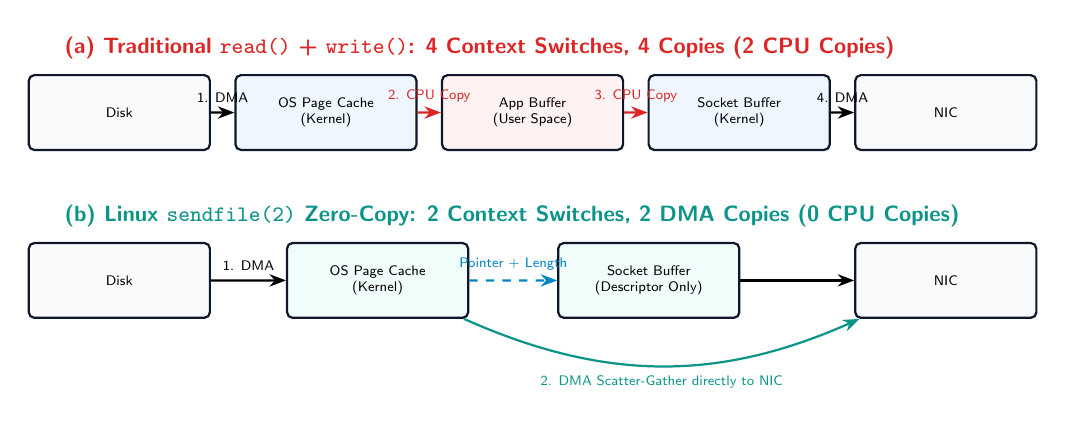
\begin{tikzpicture}[
  scale=0.82,
  box/.style={rectangle, draw=headingblue, fill=codebg, thick, rounded corners=2pt, minimum width=2.3cm, minimum height=0.95cm, align=center, font=\sffamily\tiny}
]
  % Top: Traditional 4-copy
  \node[anchor=west, font=\sffamily\bfseries\footnotesize, color=warningRed] at (0, 2.3) {(a) Traditional \texttt{read()} + \texttt{write()}: 4 Context Switches, 4 Copies (2 CPU Copies)};
  \node[box] (d1) at (1.0, 1.3) {Disk};
  \node[box, fill=exampleBg] (pc1) at (4.2, 1.3) {OS Page Cache\\(Kernel)};
  \node[box, fill=warningBg] (usr1) at (7.4, 1.3) {App Buffer\\(User Space)};
  \node[box, fill=exampleBg] (sk1) at (10.6, 1.3) {Socket Buffer\\(Kernel)};
  \node[box] (nic1) at (13.8, 1.3) {NIC};

  \draw[-{Stealth[scale=0.9]}, thick] (d1) -- node[above, font=\sffamily\tiny] {1. DMA} (pc1);
  \draw[-{Stealth[scale=0.9]}, thick, color=warningRed] (pc1) -- node[above, font=\sffamily\tiny] {2. CPU Copy} (usr1);
  \draw[-{Stealth[scale=0.9]}, thick, color=warningRed] (usr1) -- node[above, font=\sffamily\tiny] {3. CPU Copy} (sk1);
  \draw[-{Stealth[scale=0.9]}, thick] (sk1) -- node[above, font=\sffamily\tiny] {4. DMA} (nic1);

  % Bottom: Zero-copy sendfile
  \node[anchor=west, font=\sffamily\bfseries\footnotesize, color=intuitionTeal] at (0, -0.3) {(b) Linux \texttt{sendfile(2)} Zero-Copy: 2 Context Switches, 2 DMA Copies (0 CPU Copies)};
  \node[box] (d2) at (1.0, -1.3) {Disk};
  \node[box, fill=intuitionBg] (pc2) at (5.0, -1.3) {OS Page Cache\\(Kernel)};
  \node[box, fill=intuitionBg] (sk2) at (9.2, -1.3) {Socket Buffer\\(Descriptor Only)};
  \node[box] (nic2) at (13.8, -1.3) {NIC};

  \draw[-{Stealth[scale=0.9]}, thick] (d2) -- node[above, font=\sffamily\tiny] {1. DMA} (pc2);
  \draw[-{Stealth[scale=0.9]}, thick, dashed, color=linkblue] (pc2) -- node[above, font=\sffamily\tiny] {Pointer + Length} (sk2);
  \draw[-{Stealth[scale=0.9]}, thick, color=intuitionTeal] (pc2) to [bend right=24] node[below, font=\sffamily\tiny] {2. DMA Scatter-Gather directly to NIC} (nic2);
  \draw[-{Stealth[scale=0.9]}, thick] (sk2) -- (nic2);
\end{tikzpicture}
\caption{Side-by-Side Comparison: Traditional 4-Copy Path vs. Kafka \texttt{sendfile(2)} Zero-Copy}
\label{fig:v4-ch05-zero-copy-comparison}
\end{figure}

Kafka replaces \texttt{read()}+\texttt{write()} with the Linux \texttt{sendfile(2)} syscall (Figure~\ref{fig:v4-ch05-zero-copy-comparison}, bottom). Only a tiny descriptor (memory offset and byte count) is placed in the Socket Buffer, and the NIC reads directly from the OS Page Cache via DMA scatter-gather. Data never crosses into JVM user space---cutting CPU copies to \textbf{zero} (note: TLS encryption in user space prevents kernel zero-copy unless kernel TLS, \texttt{kTLS}, is enabled).

\section{Apache Kafka Internals}

Designed at LinkedIn in 2010, Kafka models messaging as a distributed, partitioned, replicated append-only commit log.

\subsection{Commit Log Segments and Sparse Index}

A Kafka \textbf{Topic} is split into ordered \textbf{Partitions}. On disk, each partition directory stores rolling $1\text{ GB}$ \textbf{segment files}:
\begin{lstlisting}[language=bash]
/var/lib/kafka/data/orders-0/
    00000000000000000000.log        # Records starting at offset 0
    00000000000000000000.index      # Offset -> byte position sparse map
    00000000000000000000.timeindex  # Timestamp -> offset sparse map
\end{lstlisting}

\begin{figure}[htbp]
\centering
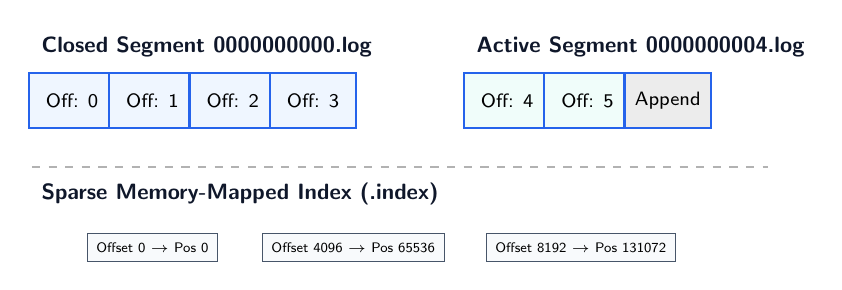
\begin{tikzpicture}[
  scale=0.85,
  entry/.style={rectangle, draw=exampleBlue, fill=exampleBg, thick, minimum width=1.1cm, minimum height=0.7cm, font=\sffamily\scriptsize}
]
  \node[anchor=west, font=\sffamily\bfseries\footnotesize, color=headingblue] at (0, 2.2) {Closed Segment 0000000000.log};
  \node[entry] (e0) at (0.6, 1.4) {Off: 0};
  \node[entry] (e1) at (1.8, 1.4) {Off: 1};
  \node[entry] (e2) at (3.0, 1.4) {Off: 2};
  \node[entry] (e3) at (4.2, 1.4) {Off: 3};

  \node[anchor=west, font=\sffamily\bfseries\footnotesize, color=headingblue] at (6.5, 2.2) {Active Segment 0000000004.log};
  \node[entry, fill=intuitionBg] (e4) at (7.1, 1.4) {Off: 4};
  \node[entry, fill=intuitionBg] (e5) at (8.3, 1.4) {Off: 5};
  \node[entry, fill=gray!15] (e6) at (9.5, 1.4) {Append};

  \draw[thick, dashed, color=gray!60] (0, 0.4) -- (11, 0.4);
  \node[anchor=west, font=\sffamily\bfseries\footnotesize, color=headingblue] at (0, 0.0) {Sparse Memory-Mapped Index (.index)};

  \node[rectangle, draw=hoodSlate, fill=hoodBg, font=\sffamily\tiny, align=center] at (1.8, -0.8) {Offset 0 $\to$ Pos 0};
  \node[rectangle, draw=hoodSlate, fill=hoodBg, font=\sffamily\tiny, align=center] at (4.8, -0.8) {Offset 4096 $\to$ Pos 65536};
  \node[rectangle, draw=hoodSlate, fill=hoodBg, font=\sffamily\tiny, align=center] at (8.2, -0.8) {Offset 8192 $\to$ Pos 131072};
\end{tikzpicture}
\caption{Kafka Segmented Commit Log and Sparse Memory-Mapped Index}
\label{fig:v4-ch05-kafka-segments}
\end{figure}

Rather than indexing every single message, Kafka writes an entry to \texttt{.index} roughly every $4\text{ KB}$ (\texttt{index.interval.bytes}). To fetch offset $4{,}120$, Kafka binary-searches the memory-mapped \texttt{.index} to find the nearest entry $\le 4{,}120$ (offset $4{,}096$ at byte $65{,}536$) and scans forward sequentially a few kilobytes inside the \texttt{.log} file.

\subsection{Replication Topology: ISR, High Watermark, and KRaft}

Every partition has one \textbf{Leader} broker handling reads/writes and zero or more \textbf{Follower} brokers pulling updates:
\begin{itemize}[leftmargin=18pt]
  \item \textbf{In-Sync Replicas (ISR)}: Followers caught up within \texttt{replica.lag.time.max.ms} (default $30\text{ s}$).
  \item \textbf{Log End Offset (LEO)}: Offset of the next record to be appended on a replica.
  \item \textbf{High Watermark (HW)}: The minimum LEO across all brokers in the ISR. Consumers are only allowed to read up to the High Watermark so they never observe uncommitted records that could vanish on leader failover.
\end{itemize}

\begin{figure}[htbp]
\centering
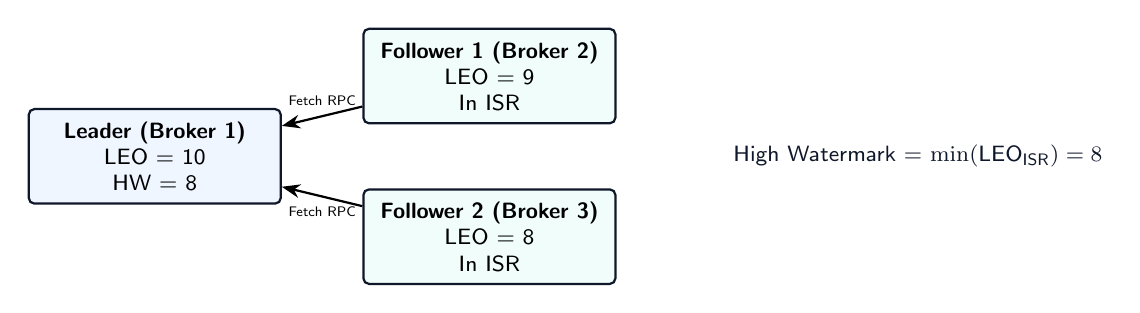
\begin{tikzpicture}[
  scale=0.85,
  nodebox/.style={rectangle, draw=headingblue, fill=codebg, thick, rounded corners=2pt, minimum width=3.2cm, minimum height=1.2cm, align=center, font=\sffamily\footnotesize}
]
  \node[nodebox, fill=exampleBg] (leader) at (0, 0) {\textbf{Leader (Broker 1)}\\LEO = 10\\HW = 8};
  \node[nodebox, fill=intuitionBg] (f1) at (5, 1.2) {\textbf{Follower 1 (Broker 2)}\\LEO = 9\\In ISR};
  \node[nodebox, fill=intuitionBg] (f2) at (5, -1.2) {\textbf{Follower 2 (Broker 3)}\\LEO = 8\\In ISR};

  \draw[-{Stealth[scale=1.0]}, thick] (f1) -- node[above, font=\sffamily\tiny] {Fetch RPC} (leader);
  \draw[-{Stealth[scale=1.0]}, thick] (f2) -- node[below, font=\sffamily\tiny] {Fetch RPC} (leader);

  \node[anchor=west, font=\sffamily\footnotesize, color=headingblue] at (8.5, 0) {High Watermark = $\min(\text{LEO}_{\text{ISR}}) = 8$};
\end{tikzpicture}
\caption{Kafka ISR Replication and High Watermark Calculation}
\label{fig:v4-ch05-kafka-hw}
\end{figure}

Historically, Kafka stored cluster topology and partition leaders in Apache ZooKeeper, capping clusters around $\sim 200{,}000$ partitions due to ZooKeeper memory reload times on failover. Under \textbf{KRaft} (Kafka Raft Metadata Mode, KIP-500), ZooKeeper is removed entirely: dedicated controller nodes run Raft consensus over an internal replicated log topic named \textbf{\texttt{\_\_cluster\_metadata}}, enabling millions of partitions and sub-second controller failovers.

\subsection{Producer Batching and Kafka 3.0+ Idempotent Defaults}

Sending one network packet per $200\text{-byte}$ JSON event wastes TCP overhead. Instead, Kafka producers accumulate records in RAM (\texttt{buffer.memory}, default $32\text{ MB}$) into per-partition batches. A sender thread dispatches a batch as soon as \emph{either}:
\begin{enumerate}[leftmargin=18pt]
  \item The batch reaches \texttt{batch.size} (default $16{,}384$ bytes), \textbf{or}
  \item \texttt{linger.ms} expires (default $0\text{ ms}$; setting $10\text{--}20\text{ ms}$ lets batches fill cleanly under load).
\end{enumerate}
If records sit in the accumulator longer than \texttt{delivery.timeout.ms} (default $120{,}000\text{ ms}$) due to downstream slowness or uncompressed payloads saturating bandwidth, the producer raises \texttt{TimeoutException}.

Since Kafka~3.0, producers enable \texttt{acks=all}, \texttt{enable.idempotence=true}, and \texttt{max.in.flight.requests.per.connection=5} by default. Why is \texttt{5} safe? Without idempotence, allowing 5 unacknowledged requests on the wire risks reordering if batch~1 fails and retries behind batch~2. With idempotence enabled, the producer stamps each batch with a monotonically increasing sequence number; the broker rejects out-of-order or duplicate sequences, giving both high pipelined throughput and strict per-partition ordering!

\subsection{Consumer Groups and Rebalance Strategies}

Within a single \textbf{Consumer Group}, Kafka guarantees that each partition is assigned to \textbf{at most one} consumer instance at a time (if you have 3 partitions and 4 workers, the 4th worker stays idle). When a worker joins, crashes, or misses its heartbeat, the group coordinator runs a partition reassignment (\textbf{rebalance}):
\begin{itemize}[leftmargin=18pt]
  \item \textbf{\texttt{RangeAssignor}} (eager): Assigns contiguous partition slices per topic (e.g., Topic~A partitions 0--1 to C1, 2 to C2). On rebalance, every consumer revokes all partitions and stops reading until reassignment completes (a stop-the-world stall).
  \item \textbf{\texttt{RoundRobinAssignor}} (eager): Stripes partitions across consumers evenly across all subscribed topics, preventing skew when topics have few partitions, but still halts all consumers during rebalance.
  \item \textbf{\texttt{CooperativeStickyAssignor}} (incremental): Keeps existing assignments intact and revokes \emph{only} the specific partitions that need to move to a new or surviving consumer. Unaffected partitions keep streaming with zero downtime.
\end{itemize}

\begin{lstlisting}[language=Python, caption={Kafka Idempotent Producer and Cooperative Consumer in Python (\texttt{confluent\_kafka})}]
import json
from confluent_kafka import Producer, Consumer

# 1. Producer with batching, LZ4 compression, and Kafka 3.0+ safety defaults
producer = Producer({
    "bootstrap.servers": "kafka-1:9092,kafka-2:9092",
    "acks": "all",
    "enable.idempotence": True,
    "max.in.flight.requests.per.connection": 5,
    "compression.type": "lz4",
    "batch.size": 65536,   # 64 KB batches
    "linger.ms": 15,       # Wait up to 15ms to fill batch
})

order = {"order_id": "ord-501", "account_id": "acct-9", "amount": 120.0}
producer.produce(
    topic="orders",
    key=order["account_id"].encode("utf-8"),
    value=json.dumps(order).encode("utf-8"),
)
producer.flush(timeout=5.0)

# 2. Consumer with CooperativeStickyAssignor and manual offset commit
consumer = Consumer({
    "bootstrap.servers": "kafka-1:9092,kafka-2:9092",
    "group.id": "billing-workers",
    "auto.offset.reset": "earliest",
    "enable.auto.commit": False,
    "partition.assignment.strategy": "cooperative-sticky",
})
consumer.subscribe(["orders"])

msg = consumer.poll(timeout=1.0)
if msg is not None and not msg.error():
    payload = json.loads(msg.value().decode("utf-8"))
    # Process payload idempotently in DB first, then commit offset
    consumer.commit(message=msg, asynchronous=False)
\end{lstlisting}

\textbf{Step-by-step walkthrough:}
\begin{enumerate}[leftmargin=18pt]
  \item Lines~5--13 configure the producer to require ISR quorum confirmation (\texttt{acks="all"}), prevent retry duplicates/reordering (\texttt{enable.idempotence=True} with \texttt{max.in.flight=5}), compress batches with LZ4, and buffer up to $64\text{ KB}$ or $15\text{ ms}$.
  \item Lines~15--21 key the message by \texttt{"acct-9"}. Kafka hashes the key (\texttt{murmur2(key) \% num\_partitions}) so all events for \texttt{acct-9} always land on the same partition in strict chronological order; \texttt{flush()} blocks until the broker ISR acknowledges.
  \item Lines~24--32 create a consumer in group \texttt{"billing-workers"} disabling auto-commit (so offsets never advance before DB writes succeed) and enabling \texttt{"cooperative-sticky"} incremental rebalancing.
  \item Lines~34--38 poll one record, decode the JSON order, and call synchronous \texttt{commit(message=msg)} only \emph{after} processing completes, enforcing at-least-once semantics.
\end{enumerate}

\section{RabbitMQ Internals}

Written in Erlang/OTP and implementing the \textbf{AMQP 0-9-1} protocol, RabbitMQ excels at smart routing, task prioritization, and per-message acknowledgments rather than multi-day log retention.

\subsection{AMQP 0-9-1 Exchanges and Bindings}

In RabbitMQ, producers never publish directly to queues. They publish to an \textbf{Exchange}, which evaluates rules called \textbf{Bindings} to route copies into one or more \textbf{Queues}:
\begin{enumerate}[leftmargin=18pt]
  \item \textbf{Direct}: Routes when the message's routing key equals the binding key exactly.
  \item \textbf{Fanout}: Ignores routing keys; broadcasts copies to every bound queue.
  \item \textbf{Topic}: Matches dot-separated words using \texttt{*} (exactly one word) and \texttt{\#} (zero or more words).
  \item \textbf{Headers}: Routes using arbitrary key-value attributes in message headers.
\end{enumerate}

\begin{figure}[htbp]
\centering
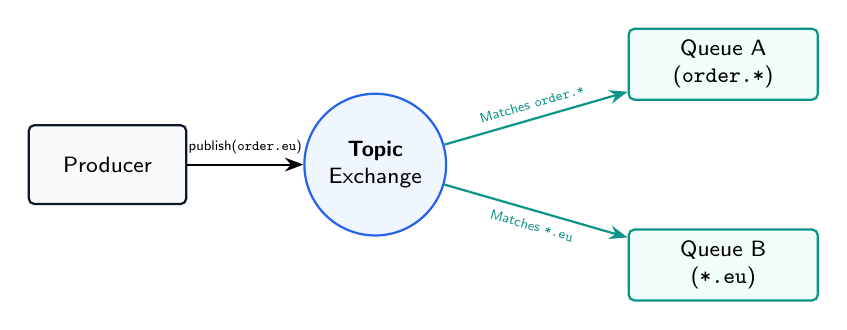
\begin{tikzpicture}[
  scale=0.85,
  p/.style={rectangle, draw=headingblue, fill=codebg, thick, rounded corners=2pt, minimum width=2.0cm, minimum height=1.0cm, align=center, font=\sffamily\footnotesize},
  ex/.style={circle, draw=exampleBlue, fill=exampleBg, thick, minimum size=1.8cm, align=center, font=\sffamily\footnotesize},
  q/.style={rectangle, draw=intuitionTeal, fill=intuitionBg, thick, rounded corners=2pt, minimum width=2.4cm, minimum height=0.9cm, align=center, font=\sffamily\footnotesize}
]
  \node[p] (prod) at (0, 0) {Producer};
  \node[ex] (exch) at (4, 0) {\textbf{Topic}\\Exchange};
  \node[q] (q1) at (9.2, 1.5) {Queue A\\(\texttt{order.*})};
  \node[q] (q2) at (9.2, -1.5) {Queue B\\(\texttt{*.eu})};

  \draw[-{Stealth[scale=1.0]}, thick] (prod) -- node[above, font=\sffamily\tiny] {publish(\texttt{order.eu})} (exch);
  \draw[-{Stealth[scale=1.0]}, thick, color=intuitionTeal] (exch) -- node[above, sloped, font=\sffamily\tiny] {Matches \texttt{order.*}} (q1);
  \draw[-{Stealth[scale=1.0]}, thick, color=intuitionTeal] (exch) -- node[below, sloped, font=\sffamily\tiny] {Matches \texttt{*.eu}} (q2);
\end{tikzpicture}
\caption{RabbitMQ AMQP 0-9-1 Topic Exchange Routing Topology}
\label{fig:v4-ch05-amqp-routing}
\end{figure}

\begin{lstlisting}[language=Python, caption={RabbitMQ Topic Exchange, Prefetch, and Manual Ack in Python (\texttt{pika})}]
import json
import pika

conn = pika.BlockingConnection(pika.ConnectionParameters("rabbitmq-1"))
ch = conn.channel()

# Declare a durable topic exchange and queue, then bind with wildcard pattern
ch.exchange_declare(exchange="orders_ex", exchange_type="topic", durable=True)
ch.queue_declare(queue="eu_orders", durable=True, arguments={"x-queue-type": "quorum"})
ch.queue_bind(queue="eu_orders", exchange="orders_ex", routing_key="order.*.eu")

# Publish a persistent message matching "order.created.eu"
ch.basic_publish(
    exchange="orders_ex",
    routing_key="order.created.eu",
    body=json.dumps({"order_id": "ord-501"}).encode("utf-8"),
    properties=pika.BasicProperties(delivery_mode=2),  # Persist to disk
)

# Consume safely with bounded prefetch backpressure
ch.basic_qos(prefetch_count=50)
method, props, body = ch.basic_get(queue="eu_orders", auto_ack=False)
if method is not None:
    data = json.loads(body.decode("utf-8"))
    ch.basic_ack(delivery_tag=method.delivery_tag)
conn.close()
\end{lstlisting}

\textbf{Step-by-step walkthrough:}
\begin{enumerate}[leftmargin=18pt]
  \item Lines~8--10 declare a durable topic exchange \texttt{orders\_ex}, a Raft-backed \texttt{quorum} queue \texttt{eu\_orders}, and a binding \texttt{order.*.eu} (note \texttt{*} matches one word, \texttt{created}).
  \item Lines~13--18 publish \texttt{\{"order\_id": "ord-501"\}} with routing key \texttt{order.created.eu} and \texttt{delivery\_mode=2} (persistent on disk). The exchange matches \texttt{order.*.eu} and routes the message into \texttt{eu\_orders}.
  \item Lines~21--25 bound unacked deliveries to 50 (\texttt{basic\_qos}), fetch the message with \texttt{auto\_ack=False}, parse the JSON, and send \texttt{basic\_ack(delivery\_tag)} so the queue deletes the message only after completion.
\end{enumerate}

\subsection{Erlang BEAM Reductions, Mnesia, and Quorum Queues}

RabbitMQ runs on the Erlang **BEAM** virtual machine, where every TCP connection, AMQP channel, and queue is an isolated lightweight **actor process** ($\sim 2.5\text{ KB}$ memory, sharing no state and communicating via async messages).
\begin{itemize}[leftmargin=18pt]
  \item \textbf{BEAM Reductions}: Rather than letting one busy queue monopolize a CPU core, the BEAM scheduler tracks work using \textbf{reductions} (an abstract counter roughly equal to one function call or built-in operation). After **4,000 reductions**, BEAM preempts the actor and schedules the next waiting actor---ensuring smooth tail latency across hundreds of thousands of queues.
  \item \textbf{Mnesia}: Erlang's built-in distributed database stores cluster metadata (users, vhosts, exchanges, queue definitions, and binding rules) in RAM and on disk across broker nodes.
  \item \textbf{Classic Mirrored Queues vs. Quorum Queues}: Legacy Classic Mirrored Queues used primary/mirror replication that silently dropped un-synced messages on crash and froze traffic during resynchronization. Modern **Quorum Queues** (RabbitMQ 3.8+, set via \texttt{x-queue-type: quorum}) implement **Raft consensus** per queue across an odd number of brokers ($3$ or $5$), surviving crashes with zero message loss and non-blocking catch-up.
\end{itemize}

\begin{realworldbox}[Diagnosing a Kafka Consumer Rebalance Storm]
\textbf{Symptom:} A \texttt{billing-workers} deployment repeatedly logs \texttt{CommitFailedException} and consumer lag climbs to 500,000 messages while CPU sits below 20\%.\\
\textbf{Sample Broker / Client Logs:}
\begin{verbatim}
[Consumer group=billing-workers] Member consumer-3-a81f exceeded max.poll.interval.ms
(300000 ms) and was kicked out of the group. Triggering rebalance (generation 47 -> 48).
CommitFailedException: Commit cannot be completed since the group has already rebalanced.
\end{verbatim}
\textbf{Root Cause \& Fix:} A slow downstream API call stalled a worker's loop for $>5\text{ minutes}$ between \texttt{poll()} calls, causing the coordinator to evict the worker and trigger an eager rebalance storm across the whole group. Lower \texttt{max.poll.records} (e.g., from 500 to 50) so each batch finishes well inside \texttt{max.poll.interval.ms}, switch to \texttt{CooperativeStickyAssignor}, and offload slow calls or set strict HTTP timeouts.
\end{realworldbox}

\begin{tryityourselfbox}[Trace Partition Assignment and AMQP Wildcards]
\begin{enumerate}[leftmargin=18pt]
  \item Suppose Topic~T1 has 4 partitions ($P_0..P_3$) and Topic~T2 has 4 partitions ($P_0..P_3$). A consumer group has 2 workers ($C_1, C_2$) subscribed to both topics. List the exact partition assignment under \texttt{RangeAssignor} vs. \texttt{RoundRobinAssignor}. What happens if a 3rd worker $C_3$ joins under \texttt{RangeAssignor}?
  \item Which of the following AMQP routing keys match a binding of \texttt{payments.\#.failed}: (a) \texttt{payments.failed}, (b) \texttt{payments.eu.card.failed}, (c) \texttt{payments.card.succeeded}?
\end{enumerate}
\end{tryityourselfbox}

\section{Summary \protect\& Key Takeaways}
\begin{itemize}[leftmargin=18pt]
  \item Kafka pairs sequential disk appends, sparse \texttt{.index} binary search, the Linux OS Page Cache, and \texttt{sendfile(2)} zero-copy (2 DMA copies, 0 CPU copies) to deliver multi-GB/s throughput without JVM heap bloat.
  \item Consumers only read up to the High Watermark ($\min(\text{LEO}_{\text{ISR}})$); KRaft replaces ZooKeeper with an internal Raft topic named \texttt{\_\_cluster\_metadata}.
  \item Kafka 3.0+ defaults (\texttt{acks=all}, \texttt{enable.idempotence=true}, \texttt{max.in.flight=5}) plus \texttt{CooperativeStickyAssignor} maximize throughput without sacrificing order or triggering stop-the-world rebalances.
  \item RabbitMQ routes messages through AMQP Exchanges (Direct, Fanout, Topic, Headers), stores topology in Mnesia, schedules actors preemptively via BEAM reductions (4,000 per slice), and achieves Raft-backed HA via Quorum Queues.
\end{itemize}

\section{Exercises}

\subsection*{Exercise~\thechapter.1 (Mechanics): Partition Count vs. Consumer Scaling}
Given a Kafka topic with 3 partitions and a consumer group with 4 active workers:
\begin{enumerate}[leftmargin=18pt]
  \item How many workers actively consume records under \texttt{RangeAssignor}?
  \item What happens if one active worker crashes?
  \item Why does \texttt{CooperativeStickyAssignor} prevent full-group processing stalls during that failover?
\end{enumerate}

\subsection*{Exercise~\thechapter.2 (Debugging): Kafka Producer \texttt{TimeoutException}}
A telemetry producer throws:
\begin{lstlisting}[language=Java]
org.apache.kafka.common.errors.TimeoutException: Expiring 48 record(s) for sensors-2: 120000 ms has passed since batch creation
\end{lstlisting}
Network links are healthy and broker CPU is 15\%. Explain how \texttt{buffer.memory}, \texttt{batch.size}, \texttt{linger.ms}, \texttt{compression.type}, and \texttt{delivery.timeout.ms} interact to cause and fix this error.

\subsection*{Exercise~\thechapter.3 (Architecture): Selecting Kafka vs. RabbitMQ}
Justify choosing Kafka or RabbitMQ for:
\begin{enumerate}[leftmargin=18pt]
  \item A core ledger event backbone needing 7-year replayable audit history, strict per-account ordering, and fraud-detection stream joins.
  \item A multi-step PDF/video rendering dispatcher needing VIP priority queues, wildcard routing to GPU/CPU pools, and immediate deletion upon task completion.
\end{enumerate}

\subsection*{Exercise~\thechapter.4 (Try-It-Yourself Lab): Assignor Trace & AMQP Topic Matching}
Solve both parts of the \emph{Try It Yourself} box above.

\section{Detailed Solutions}

\subsection*{Solution to Exercise~\thechapter.1}
\begin{enumerate}[leftmargin=18pt]
  \item At most one worker per partition in a group means \textbf{3 workers} consume partitions ($P_0, P_1, P_2$) while the 4th worker remains idle standby.
  \item On crash, the coordinator detects missed heartbeats and reassigns the orphaned partition to the idle 4th worker.
  \item Eager assignors revoke \emph{all} partitions from all workers before reassigning. \texttt{CooperativeStickyAssignor} keeps unaffected partitions running continuously and migrates only the single orphaned partition.
\end{enumerate}

\subsection*{Solution to Exercise~\thechapter.2}
Uncompressed JSON telemetry fills \texttt{buffer.memory} faster than the sender thread can drain tiny $16\text{ KB}$ batches, leaving queued batches waiting past \texttt{delivery.timeout.ms} ($120\text{ s}$). Fix by enabling \texttt{compression.type=lz4} (shrinking payloads 60--80\%), raising \texttt{batch.size=65536}, setting \texttt{linger.ms=20}, and keeping \texttt{max.in.flight.requests.per.connection=5} with \texttt{enable.idempotence=true}.

\subsection*{Solution to Exercise~\thechapter.3}
\begin{itemize}[leftmargin=18pt]
  \item \textbf{Core Ledger $\to$ Apache Kafka}: Tiered append-only storage retains 7 years of immutable events; partitioning by \texttt{account\_id} guarantees strict per-account order; Kafka Streams/Flink processes sliding fraud windows natively.
  \item \textbf{Rendering Dispatcher $\to$ RabbitMQ}: AMQP Topic exchanges route \texttt{render.gpu.*} vs. \texttt{render.cpu.*}; native priority queues (\texttt{x-max-priority}) let VIP jobs jump queues; destructive ACKs purge finished jobs immediately.
\end{itemize}

\subsection*{Solution to Exercise~\thechapter.4}
\begin{enumerate}[leftmargin=18pt]
  \item Under \texttt{RangeAssignor} (assigned per topic): $C_1$ gets \texttt{T1-0, T1-1, T2-0, T2-1}; $C_2$ gets \texttt{T1-2, T1-3, T2-2, T2-3}. Under \texttt{RoundRobinAssignor}: identical 4/4 split here, though on 3 consumers ($C_1, C_2, C_3$) \texttt{RangeAssignor} skews heavily: $C_1$ gets 2 partitions per topic (\texttt{T1-0, T1-1, T2-0, T2-1} = 4 total) while $C_2$ and $C_3$ get only 2 total each! \texttt{RoundRobinAssignor} gives a balanced 3/3/2 split.
  \item Since \texttt{\#} matches zero or more words: (a) \texttt{payments.failed} matches (0 words between), (b) \texttt{payments.eu.card.failed} matches (2 words between), (c) \texttt{payments.card.succeeded} does \emph{not} match.
\end{enumerate}

\begin{labbridgebox}[Event-Driven Outbox & Full Stack Broker Integration]
Explore Kafka-style partitioned log delivery in \texttt{projects/p11-event-driven-microservices}, and inspect live RabbitMQ exchanges, queues, and worker consumption in \texttt{projects/p12-end-to-end-platform} (ports 5672/15672).
\end{labbridgebox}

\section{Further Reading \protect\& Citations}
\begin{itemize}[leftmargin=18pt]
  \item Kreps, J., Narkhede, N., \& Rao, J. (2011). \emph{Kafka: A distributed messaging system for log processing}. NetDB Workshop, 1--7.
  \item Videla, A., \& Williams, J. (2012). \emph{RabbitMQ in Action: Distributed messaging for everyone}. Manning Publications.
  \item Armstrong, J. (2010). \emph{Erlang}. Communications of the ACM, 53(9), 68--75.
\end{itemize}

\chapter{Redis and Caching Topologies}
\label{ch:redis-caching}

\begin{chaptergoalsbox}
\textbf{What you will learn:}
\begin{itemize}[leftmargin=12pt]
  \item Why Redis uses a single-threaded non-blocking I/O event loop (\texttt{epoll}/\texttt{kqueue}) and how its C structures (\texttt{sds}, \texttt{dict}, \texttt{skiplist}, and \texttt{listpack} replacing \texttt{ziplist}) optimize RAM and CPU cache locality.
  \item Approximated LRU and probabilistic Morris-counter LFU memory eviction.
  \item Caching topologies in Python: Cache-Aside, Read-Through, Write-Through, and Write-Behind.
  \item Defending against Stampedes (XFetch), Penetration (Bloom filters), Avalanches (TTL jitter), and atomic Lua scripts using \texttt{HSET}.
  \item Redis Sentinel failover vs. Redis Cluster 16,384 hash slots, hash tags, and \texttt{-MOVED} redirects.
\end{itemize}

\textbf{What you should already understand:}
\begin{itemize}[leftmargin=12pt]
  \item Basic key-value operations (\texttt{GET}, \texttt{SET}, \texttt{DEL}) and relational SQL queries.
  \item Network round-trip costs from Chapter~\ref{ch:distributed-fundamentals}; no prior C data-structure internals are assumed.
\end{itemize}

\textbf{Why this topic exists:}
Reading a row from DRAM takes $\sim 100\text{ ns}$, whereas querying a relational database on disk or joining tables under lock contention takes milliseconds---ten thousand times slower. Yet teams that slap Redis in front of a database without understanding eviction, stampedes, or write invalidation routinely trade slow pages for silent stale data and midnight outages.

\textbf{Motivating practical problem:}
An airline ticketing portal caches flight-availability searches with a fixed 24-hour TTL expiring at 00:00 UTC. At 00:00:01, 80,000 concurrent browsers miss Redis simultaneously and slam PostgreSQL with identical complex queries. Database connections saturate, disk queues spike, and the booking platform stays down for 45 minutes.
\end{chaptergoalsbox}

\section{Redis Architecture and Internal Data Structures}

Created by Salvatore Sanfilippo in 2009, \textbf{Redis} (Remote Dictionary Server) stores typed data structures directly in RAM while optionally persisting snapshots or append logs to disk.

\subsection{The Single-Threaded Multiplexed Event Loop}

Contrary to intuition, Redis processes all client commands on a \textbf{single main thread} (while offloading slow background tasks like large-key deletion via \texttt{UNLINK} and disk \texttt{fsync} to helper threads). Instead of spawning one OS thread per client socket, Redis registers thousands of non-blocking TCP sockets with the kernel's \textbf{I/O multiplexer} (\texttt{epoll} on Linux, \texttt{kqueue} on BSD/macOS), waking up only for sockets that actually have bytes ready to read or write.

\begin{figure}[htbp]
\centering
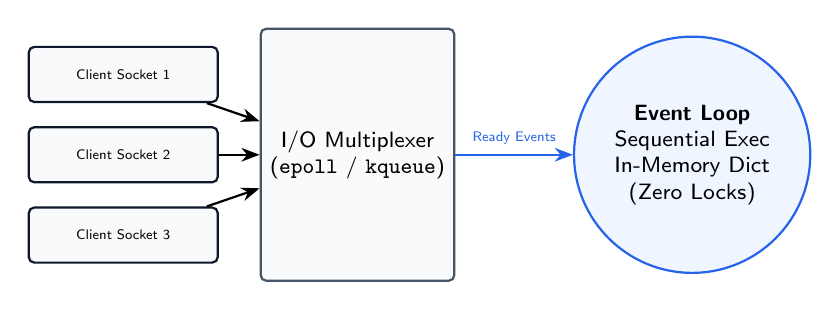
\begin{tikzpicture}[
  scale=0.85,
  sock/.style={rectangle, draw=headingblue, fill=codebg, thick, rounded corners=2pt, minimum width=2.4cm, minimum height=0.7cm, align=center, font=\sffamily\tiny},
  loop/.style={circle, draw=exampleBlue, fill=exampleBg, thick, minimum size=3.0cm, align=center, font=\sffamily\footnotesize}
]
  \node[sock] (s1) at (-4, 1.2) {Client Socket 1};
  \node[sock] (s2) at (-4, 0.0) {Client Socket 2};
  \node[sock] (s3) at (-4, -1.2) {Client Socket 3};

  \node[rectangle, draw=hoodSlate, fill=hoodBg, thick, rounded corners=2pt, minimum width=2.3cm, minimum height=3.2cm, align=center, font=\sffamily\footnotesize] (mux) at (-0.5, 0) {I/O Multiplexer\\(\texttt{epoll} / \texttt{kqueue})};

  \node[loop] (el) at (4.5, 0) {\textbf{Event Loop}\\Sequential Exec\\In-Memory Dict\\(Zero Locks)};

  \draw[-{Stealth[scale=1.0]}, thick] (s1) -- (mux);
  \draw[-{Stealth[scale=1.0]}, thick] (s2) -- (mux);
  \draw[-{Stealth[scale=1.0]}, thick] (s3) -- (mux);

  \draw[-{Stealth[scale=1.0]}, thick, color=exampleBlue] (mux) -- node[above, font=\sffamily\tiny] {Ready Events} (el);
\end{tikzpicture}
\caption{Redis Single-Threaded Non-Blocking Event Loop}
\label{fig:v4-ch06-event-loop}
\end{figure}

Why is single-threaded execution so fast? In-memory operations take nanoseconds, so Redis is bottlenecked by network I/O and RAM bandwidth, not CPU cores. Running commands sequentially eliminates mutex locks, deadlocks, and OS thread context-switching overhead, letting one core sustain $>100{,}000$ operations per second.

\subsection{Internal C Data Structures: SDS, Dict, SkipList, and Listpack}

\begin{itemize}[leftmargin=18pt]
  \item \textbf{SDS (Simple Dynamic String)}: In standard C, strings end at the first null byte (\texttt{'\textbackslash 0'}), forcing $O(N)$ scans to compute length and breaking on binary payloads. Redis wraps strings in \texttt{sdshdr}, storing exact length and allocated capacity upfront---giving $O(1)$ length checks, binary safety (images, Protobufs), and pre-allocated growth headroom.
  \item \textbf{Dict (Incremental Rehashing Hash Table)}: When a hash table fills up and must double in size, moving 50 million keys at once would freeze the single-threaded event loop for seconds. Redis keeps \emph{two} hash tables ($ht[0]$ and $ht[1]$) and performs \textbf{incremental rehashing}: each incoming client command migrates just one bucket from $ht[0]$ to $ht[1]$ until the resize completes smoothly.
  \item \textbf{SkipList (Sorted Sets / \texttt{ZSET})}: Imagine a highway with local exits at every mile (Level~1), express exits every few miles (Level~2), and interstate hubs (Level~3). Instead of complex tree rotations (like Red-Black trees), a SkipList builds these express lanes probabilistically: every inserted element starts at Level~1 and repeatedly ``flips a biased coin'' (probability $p = 0.25$ in Redis, up to 32 levels) to get promoted to higher express lanes. Searching from the top lane down achieves $O(\log N)$ lookups and fast range scans (\texttt{ZRANGE}).
  \item \textbf{Listpack (and Why \texttt{ziplist} Was Replaced)}: Small hashes and lists are packed contiguously into a single byte array for CPU cache efficiency. Historically, Redis used \texttt{ziplist}, where each entry stored the byte length of the \emph{previous} entry (\texttt{prevlen}) so Redis could walk backward. If \texttt{prevlen} was $< 254$ bytes, it took 1 byte; if $\ge 254$ bytes, it took 5 bytes. Inserting one 254-byte item near the front forced the next item's \texttt{prevlen} to grow from 1 to 5 bytes---pushing *that* item over 254 bytes and triggering an $O(N^2)$ \textbf{cascading reallocation} down the list! Redis~7 replaced \texttt{ziplist} with \textbf{\texttt{listpack}}, where every entry stores its \emph{own} encoding and total length at its tail. Walking backward reads the tail length in $O(1)$ with zero dependency on neighbors, completely eliminating cascading updates.
\end{itemize}

\begin{figure}[htbp]
\centering
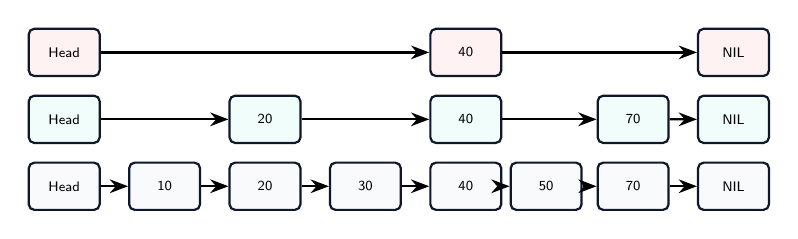
\begin{tikzpicture}[
  scale=0.85,
  node/.style={rectangle, draw=headingblue, fill=codebg, thick, rounded corners=2pt, minimum width=0.9cm, minimum height=0.6cm, align=center, font=\sffamily\tiny}
]
  \node[node, fill=warningBg] (l3_0) at (0, 2) {Head};
  \node[node, fill=warningBg] (l3_4) at (6, 2) {40};
  \node[node, fill=warningBg] (l3_8) at (10, 2) {NIL};
  \draw[-{Stealth[scale=1.0]}, thick] (l3_0) -- (l3_4);
  \draw[-{Stealth[scale=1.0]}, thick] (l3_4) -- (l3_8);

  \node[node, fill=intuitionBg] (l2_0) at (0, 1) {Head};
  \node[node, fill=intuitionBg] (l2_2) at (3, 1) {20};
  \node[node, fill=intuitionBg] (l2_4) at (6, 1) {40};
  \node[node, fill=intuitionBg] (l2_7) at (8.5, 1) {70};
  \node[node, fill=intuitionBg] (l2_8) at (10, 1) {NIL};
  \draw[-{Stealth[scale=1.0]}, thick] (l2_0) -- (l2_2);
  \draw[-{Stealth[scale=1.0]}, thick] (l2_2) -- (l2_4);
  \draw[-{Stealth[scale=1.0]}, thick] (l2_4) -- (l2_7);
  \draw[-{Stealth[scale=1.0]}, thick] (l2_7) -- (l2_8);

  \node[node] (l1_0) at (0, 0) {Head};
  \node[node] (l1_1) at (1.5, 0) {10};
  \node[node] (l1_2) at (3, 0) {20};
  \node[node] (l1_3) at (4.5, 0) {30};
  \node[node] (l1_4) at (6, 0) {40};
  \node[node] (l1_5) at (7.2, 0) {50};
  \node[node] (l1_7) at (8.5, 0) {70};
  \node[node] (l1_8) at (10, 0) {NIL};
  \draw[-{Stealth[scale=1.0]}, thick] (l1_0) -- (l1_1);
  \draw[-{Stealth[scale=1.0]}, thick] (l1_1) -- (l1_2);
  \draw[-{Stealth[scale=1.0]}, thick] (l1_2) -- (l1_3);
  \draw[-{Stealth[scale=1.0]}, thick] (l1_3) -- (l1_4);
  \draw[-{Stealth[scale=1.0]}, thick] (l1_4) -- (l1_5);
  \draw[-{Stealth[scale=1.0]}, thick] (l1_5) -- (l1_7);
  \draw[-{Stealth[scale=1.0]}, thick] (l1_7) -- (l1_8);
\end{tikzpicture}
\caption{Multi-Level SkipList Structure Supporting $O(\log N)$ Sorted Set Lookups}
\label{fig:v4-ch06-skiplist}
\end{figure}

\section{Memory Eviction: Approximated LRU and Morris LFU}

When Redis memory hits \texttt{maxmemory}, it applies the configured eviction policy (\texttt{noeviction}, \texttt{allkeys-lru}, \texttt{volatile-lru}, \texttt{allkeys-lfu}, or \texttt{volatile-lfu}).

\begin{underthehoodbox}[Sampled LRU and the Morris Counter Intuition for LFU]
True LRU needs a global doubly linked list updated on every read, wasting 16 bytes of pointers per key. Instead, Redis stores a 24-bit clock field inside each object and samples $N$ random keys (default $N=5$), evicting the oldest among the sample. With $N=10$, accuracy matches exact LRU within 1\%.

Under \textbf{LFU (Least Frequently Used)}, Redis packs both a 16-bit decay timestamp and an 8-bit frequency counter into that same 24-bit field. How can an 8-bit integer (max value $255$) distinguish $1{,}000$ hits from $1{,}000{,}000$ hits? Using a probabilistic \textbf{Morris counter}: when a key at counter $c$ is accessed, Redis increments $c$ only with probability $p = \frac{1}{(c - 5) \cdot \text{lfu-log-factor} + 1}$. As $c$ grows, increments become rarer---turning 8 bits into a compact logarithmic estimator of millions of requests!
\end{underthehoodbox}

\section{Caching Topologies with Runnable Code}

\begin{figure}[htbp]
\centering
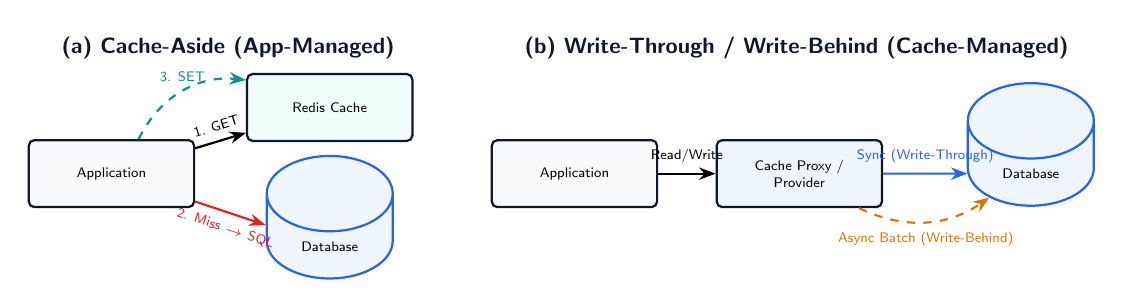
\begin{tikzpicture}[
  scale=0.84,
  box/.style={rectangle, draw=headingblue, fill=codebg, thick, rounded corners=2pt, minimum width=2.1cm, minimum height=0.85cm, align=center, font=\sffamily\tiny},
  db/.style={cylinder, draw=exampleBlue, fill=exampleBg, thick, shape border rotate=90, minimum width=1.6cm, minimum height=1.1cm, align=center, font=\sffamily\tiny}
]
  % Left: Cache-Aside
  \node[anchor=west, font=\sffamily\bfseries\footnotesize, color=headingblue] at (-0.6, 2.3) {(a) Cache-Aside (App-Managed)};
  \node[box] (app1) at (0.3, 0.4) {Application};
  \node[box, fill=intuitionBg] (c1) at (3.6, 1.4) {Redis Cache};
  \node[db] (db1) at (3.6, -0.7) {Database};
  \draw[-{Stealth[scale=0.9]}, thick] (app1) -- node[above, sloped, font=\sffamily\tiny] {1. GET} (c1);
  \draw[-{Stealth[scale=0.9]}, thick, color=warningRed] (app1) -- node[below, sloped, font=\sffamily\tiny] {2. Miss $\to$ SQL} (db1);
  \draw[-{Stealth[scale=0.9]}, thick, dashed, color=intuitionTeal] (app1) to [bend left=35] node[above, font=\sffamily\tiny] {3. SET} (c1);

  % Right: Write-Through vs Write-Behind
  \node[anchor=west, font=\sffamily\bfseries\footnotesize, color=headingblue] at (6.4, 2.3) {(b) Write-Through / Write-Behind (Cache-Managed)};
  \node[box] (app2) at (7.3, 0.4) {Application};
  \node[box, fill=exampleBg] (c2) at (10.7, 0.4) {Cache Proxy /\\Provider};
  \node[db] (db2) at (14.2, 0.4) {Database};
  \draw[-{Stealth[scale=0.9]}, thick] (app2) -- node[above, font=\sffamily\tiny] {Read/Write} (c2);
  \draw[-{Stealth[scale=0.9]}, thick, color=exampleBlue] (c2) -- node[above, font=\sffamily\tiny] {Sync (Write-Through)} (db2);
  \draw[-{Stealth[scale=0.9]}, thick, dashed, color=mistakeAmber] (c2) to [bend right=30] node[below, font=\sffamily\tiny] {Async Batch (Write-Behind)} (db2);
\end{tikzpicture}
\caption{Cache-Aside vs. Write-Through and Write-Behind Topologies}
\label{fig:v4-ch06-write-topologies}
\end{figure}

\begin{enumerate}[leftmargin=18pt]
  \item \textbf{Cache-Aside (Lazy Loading)}: The application checks Redis first; on a miss, it queries PostgreSQL and writes back to Redis with a jittered TTL. On writes, it updates PostgreSQL and \emph{deletes} the cache key.
  \item \textbf{Read-Through}: The application talks only to a caching library/proxy, which automatically loads from the database on misses so caller code stays clean.
  \item \textbf{Write-Through}: Writes go through the cache, which updates the database synchronously before acknowledging---strong consistency, higher write latency.
  \item \textbf{Write-Behind (Write-Back)}: Writes return immediately after updating cache memory; a background flusher batches updates to the database asynchronously. Extreme write speed, but risks data loss if the cache node crashes before flushing.
\end{enumerate}

\begin{lstlisting}[language=Python, caption={Cache-Aside and Read-Through with TTL Jitter in Python}]
import json
import random
from typing import Callable, Optional

def get_flight_cache_aside(redis_client, db, route_key: str, base_ttl: int = 300) -> dict:
    cache_key = f"flight:{route_key}"
    cached = redis_client.get(cache_key)
    if cached is not None:
        return json.loads(cached)

    # Cache miss: query relational DB and store with TTL jitter
    row = db.fetch_flight(route_key)
    jitter = random.randint(0, 60)  # Spread expirations across 60s window
    redis_client.set(cache_key, json.dumps(row), ex=base_ttl + jitter)
    return row

def update_flight_price(redis_client, db, route_key: str, new_price: int) -> None:
    db.update_price(route_key, new_price)
    redis_client.delete(f"flight:{route_key}")  # Invalidate, never SET blindly!

class ReadThroughCache:
    def __init__(self, redis_client, loader: Callable[[str], Optional[dict]], ttl: int = 300):
        self.redis = redis_client
        self.loader = loader
        self.ttl = ttl

    def get(self, key: str) -> Optional[dict]:
        raw = self.redis.get(key)
        if raw is not None:
            return json.loads(raw)
        data = self.loader(key)
        if data is not None:
            self.redis.set(key, json.dumps(data), ex=self.ttl + random.randint(0, 30))
        return data
\end{lstlisting}

\textbf{Step-by-step trace:}
\begin{enumerate}[leftmargin=18pt]
  \item Call \texttt{get\_flight\_cache\_aside(..., "NYC-LON")}: checks \texttt{flight:NYC-LON}. On a cold cache, \texttt{cached} is \texttt{None}, so it queries \texttt{db.fetch\_flight("NYC-LON")} (returning \texttt{\{"price": 420\}}), picks random \texttt{jitter = 23}, stores the JSON with \texttt{ex=323} seconds, and returns the dict.
  \item Subsequent calls hit Redis directly until 323s elapse. Because 10,000 keys receive random TTLs between 300s and 360s instead of expiring together, a \textbf{Cache Avalanche} at midnight is prevented.
  \item Calling \texttt{update\_flight\_price} commits to PostgreSQL and \emph{deletes} the cache key rather than calling \texttt{SET}, avoiding the stale-overwrite race where an older thread writes an outdated value after a newer thread updated the DB.
\end{enumerate}

\section{Cache Pathologies and Defenses (XFetch, Bloom Filters, Lua)}

\begin{table}[htbp]
\centering\small
\begin{tabular}{lp{4.8cm}p{6.2cm}}
\toprule
\textbf{Pathology} & \textbf{Mechanism} & \textbf{Production Defense} \\
\midrule
\textbf{Cache Stampede (Thundering Herd)} & Hot key expires; thousands of concurrent threads miss together and hit DB. & \textbf{XFetch} probabilistic early refresh or singleflight/mutex lock. \\
\textbf{Cache Penetration} & Attackers query nonexistent keys (e.g., ID \texttt{-999}) missing both cache and DB. & \textbf{Bloom Filter} ingress guard or caching short-TTL null tombstones. \\
\textbf{Cache Avalanche} & Huge batch of keys expires at the same timestamp (e.g., 00:00 UTC). & \textbf{TTL Jitter}: $\text{TTL} = \text{base} + \text{rand}(0, \Delta)$. \\
\textbf{Cache Breakdown} & One extreme celebrity hot key expires under huge QPS. & Async background refresh before expiry or logical soft-TTL inside value. \\
\bottomrule
\end{tabular}
\caption{Taxonomy of Distributed Caching Pathologies and Defenses}
\label{tab:v4-ch06-pathologies}
\end{table}

\subsection{Probabilistic Early Expiration: The XFetch Algorithm}

Why does $-\beta \cdot \delta \cdot \ln(\text{rand}()) > \text{TTL}_{\text{remaining}}$ stop stampedes without locks? Because when $u \sim \text{Uniform}(0, 1]$, $-\ln(u)$ follows an exponential distribution (mostly near $0.5\text{--}2.0$, occasionally larger). Multiplying by $\beta \cdot \delta$ (where $\delta$ is how long the DB query takes to recompute) means: when $\text{TTL}_{\text{remaining}}$ is large (say $250\text{ s}$), the threshold is virtually never crossed; as $\text{TTL}_{\text{remaining}}$ shrinks down toward $\delta$ (say $0.2\text{ s}$), \emph{one} lucky reader triggers an early refresh and resets the TTL before the key actually expires for everyone else!

\begin{figure}[htbp]
\centering
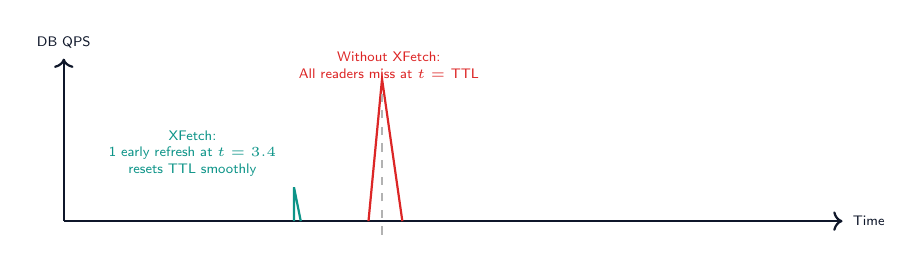
\begin{tikzpicture}[
  scale=0.86,
  axis/.style={->, thick, color=headingblue}
]
  \draw[axis] (0, 0) -- (11.5, 0) node[right, font=\sffamily\tiny] {Time};
  \draw[axis] (0, 0) -- (0, 2.4) node[above, font=\sffamily\tiny] {DB QPS};

  \draw[thick, color=warningRed] (4.5, 0) -- (4.7, 2.1) -- (5.0, 0);
  \node[font=\sffamily\tiny, color=warningRed, align=center] at (4.8, 2.3) {Without XFetch:\\All readers miss at $t=\text{TTL}$};

  \draw[thick, color=intuitionTeal] (3.4, 0) -- (3.4, 0.5) -- (3.5, 0);
  \node[font=\sffamily\tiny, color=intuitionTeal, align=center] at (1.9, 1.0) {XFetch:\\1 early refresh at $t=3.4$\\resets TTL smoothly};
  \draw[dashed, color=gray!60] (4.7, -0.2) -- (4.7, 1.9);
\end{tikzpicture}
\caption{Cache Stampede Spike vs. Smooth XFetch Early Refresh}
\label{fig:v4-ch06-stampede-xfetch}
\end{figure}

\begin{lstlisting}[language=Python, caption={XFetch Stampede-Resistant Reader in Python}]
import json, math, random, time

def get_with_xfetch(redis_client, db, key: str, ttl: float = 60.0, beta: float = 1.0):
    raw = redis_client.get(key)
    now = time.time()
    if raw is not None:
        entry = json.loads(raw)
        ttl_rem = entry["expiry"] - now
        delta = entry["delta"]
        u = max(random.random(), 1e-12)  # Avoid log(0)
        if ttl_rem > 0 and (-beta * delta * math.log(u)) <= ttl_rem:
            return entry["value"]

    # Cache miss OR probabilistically selected for early refresh
    t0 = time.monotonic()
    value = db.compute_expensive_report(key)
    delta = time.monotonic() - t0
    payload = {"value": value, "delta": delta, "expiry": time.time() + ttl}
    redis_client.set(key, json.dumps(payload), ex=int(ttl) + 5)
    return value
\end{lstlisting}

\textbf{Step-by-step trace:} Suppose \texttt{ttl = 60.0}, \texttt{beta = 1.0}, and \texttt{entry = \{"value": 99, "delta": 0.5, "expiry": now + 0.3\}} (so \texttt{ttl\_rem = 0.3s}). If a reader draws \texttt{u = 0.4}, then $-\ln(0.4) \approx 0.916$, and $1.0 \times 0.5 \times 0.916 = 0.458 > 0.3$. That single reader falls through to lines~15--19, recomputes \texttt{value}, measures \texttt{delta}, and resets \texttt{expiry = time.time() + 60.0} while all other concurrent readers still get the cached \texttt{99} cleanly.

\subsection{Bloom Filter Ingress Guard}

A \textbf{Bloom filter} is a compact bit array of $m$ bits paired with $k$ independent hash functions. It supports two answers: ``\emph{definitely not in the set}'' (100\% certain, blocking nonexistent-ID attacks before they reach PostgreSQL) or ``\emph{probably in the set}'' (small tunable false-positive rate $p \approx (1 - e^{-kn/m})^k$).

\begin{lstlisting}[language=Python, caption={Tiny Concrete Bloom Filter Ingress Guard in Python}]
import hashlib

class TinyBloomFilter:
    def __init__(self, size: int = 16, num_hashes: int = 2):
        self.size = size
        self.num_hashes = num_hashes
        self.bits = [0] * size

    def _positions(self, item: str) -> list[int]:
        pos = []
        for seed in range(self.num_hashes):
            digest = hashlib.sha256(f"{seed}:{item}".encode("utf-8")).hexdigest()
            pos.append(int(digest, 16) % self.size)
        return pos

    def add(self, item: str) -> None:
        for idx in self._positions(item):
            self.bits[idx] = 1

    def might_contain(self, item: str) -> bool:
        return all(self.bits[idx] == 1 for idx in self._positions(item))
\end{lstlisting}

\textbf{Step-by-step trace:} Create \texttt{bf = TinyBloomFilter(size=16, num\_hashes=2)}. Suppose \texttt{bf.\_positions("user:101")} hashes to indices \texttt{[3, 11]}. Calling \texttt{bf.add("user:101")} sets \texttt{bits[3] = 1} and \texttt{bits[11] = 1}. Later, an attacker sends \texttt{"user:-999"}, whose positions hash to \texttt{[3, 8]}. Since \texttt{bits[8] == 0}, \texttt{might\_contain("user:-999")} returns \texttt{False} immediately---rejecting the request in microseconds without touching Redis or PostgreSQL!

\subsection{Atomic Lua Scripts in Redis}

Because Redis runs one command at a time, sending \texttt{GET} then \texttt{SET} from Python allows another client to interleave in between. Sending a **Lua script** runs all steps atomically inside the single-threaded event loop. Note that Redis~4.0+ deprecated \texttt{HMSET} in favor of multi-field **`HSET`**.

\begin{lstlisting}[language=Python, caption={Atomic Lua Cache-Counter / Token Bucket Update Using \texttt{HSET}}]
LUA_TOKEN_BUCKET = """
local key = KEYS[1]
local capacity = tonumber(ARGV[1])
local rate = tonumber(ARGV[2])
local now = tonumber(ARGV[3])

local vals = redis.call('HMGET', key, 'tokens', 'ts')
local tokens = tonumber(vals[1]) or capacity
local last_ts = tonumber(vals[2]) or now
tokens = math.min(capacity, tokens + math.max(0, now - last_ts) * rate)

if tokens >= 1 then
    tokens = tokens - 1
    redis.call('HSET', key, 'tokens', tokens, 'ts', now)
    redis.call('EXPIRE', key, math.ceil(capacity / rate))
    return 1
end
return 0
"""
\end{lstlisting}

\textbf{Step-by-step trace:} Passing \texttt{KEYS[1]="rl:api:k1"}, \texttt{ARGV=["10", "2", "1000.0"]}: on the first call, \texttt{HMGET} returns \texttt{[nil, nil]}, initializing \texttt{tokens=10, last\_ts=1000.0}. Since \texttt{tokens >= 1}, it decrements \texttt{tokens} to \texttt{9}, atomically writes both fields with \texttt{HSET}, sets a 5-second TTL, and returns \texttt{1}.

\section{Redis Clustering: Sentinel vs. Cluster}

\textbf{Redis Sentinel} monitors a single primary-replica group with heartbeats; if a quorum of Sentinels detects \texttt{ODOWN}, they promote a replica automatically, though write throughput stays capped at one machine.

\textbf{Redis Cluster} shards writes horizontally across up to 1,000 nodes by dividing the keyspace into \textbf{16,384 hash slots}. Every key maps to a slot via:
\begin{equation}
\text{slot} = \text{CRC16}(k) \pmod{16384}
\end{equation}
Cluster nodes exchange slot ownership continuously via a binary \textbf{Gossip protocol}. If a client asks Master~1 for a key belonging to slot~12000 owned by Master~3, Master~1 replies \texttt{-MOVED 12000 10.0.0.4:6379} so the client updates its routing table. To force related keys onto the same node for multi-key operations or Lua scripts, wrap the shared identifier in \textbf{Hash Tags} (e.g., \texttt{\{user:8492\}:orders} and \texttt{\{user:8492\}:profile}): Redis hashes only the substring inside \texttt{\{...\}}.

\begin{figure}[htbp]
\centering
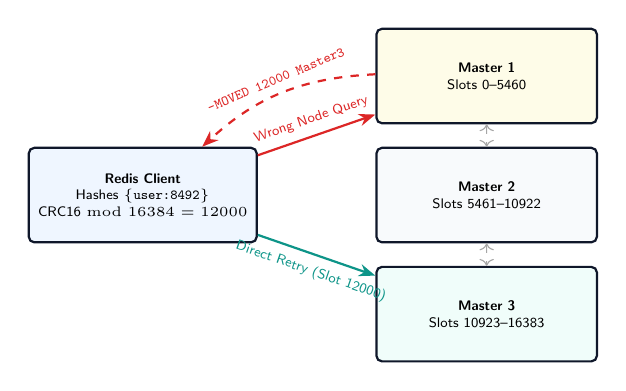
\begin{tikzpicture}[
  scale=0.84,
  box/.style={rectangle, draw=headingblue, fill=codebg, thick, rounded corners=2pt, minimum width=2.8cm, minimum height=1.2cm, align=center, font=\sffamily\tiny}
]
  \node[box, fill=exampleBg] (client) at (0, 0) {\textbf{Redis Client}\\Hashes \texttt{\{user:8492\}}\\$\text{CRC16}\bmod 16384 = 12000$};
  \node[box, fill=mistakeBg] (m1) at (5.2, 1.8) {\textbf{Master 1}\\Slots 0--5460};
  \node[box] (m2) at (5.2, 0.0) {\textbf{Master 2}\\Slots 5461--10922};
  \node[box, fill=intuitionBg] (m3) at (5.2, -1.8) {\textbf{Master 3}\\Slots 10923--16383};

  \draw[-{Stealth[scale=0.9]}, thick, color=warningRed] (client) -- node[above, sloped, font=\sffamily\tiny] {Wrong Node Query} (m1);
  \draw[-{Stealth[scale=0.9]}, thick, dashed, color=warningRed] (m1) to [bend right=20] node[above, sloped, font=\sffamily\tiny] {\texttt{-MOVED 12000 Master3}} (client);
  \draw[-{Stealth[scale=0.9]}, thick, color=intuitionTeal] (client) -- node[below, sloped, font=\sffamily\tiny] {Direct Retry (Slot 12000)} (m3);
  \draw[<->, dashed, color=gray!70] (m1) -- (m2);
  \draw[<->, dashed, color=gray!70] (m2) -- (m3);
\end{tikzpicture}
\caption{Redis Cluster 16,384 Hash-Slot Sharding and \texttt{-MOVED} Redirection}
\label{fig:v4-ch06-redis-cluster}
\end{figure}

\begin{realworldbox}[Diagnosing a Hot-Key Stampede and \texttt{CROSSSLOT} Error]
\textbf{Symptom:} Redis CPU hits 99\% on one shard while the application logs \texttt{ResponseError: CROSSSLOT Keys in request don't hash to the same slot}.\\
\textbf{Diagnostic Commands:}
\begin{verbatim}
$ redis-cli --hotkeys
# Top key: "homepage:banner" (412,000 req/s) -- TTL: 2s!
$ redis-cli INFO commandstats | grep cmdstat_mget
cmdstat_mget:calls=94000,rejected_calls=12400
\end{verbatim}
\textbf{Root Cause \& Fix:} (1) \texttt{homepage:banner} has a short TTL without XFetch, causing bursts of misses; apply XFetch or local in-process L1 caching. (2) Multi-key \texttt{MGET}/\texttt{MSET} or Lua calls across keys without matching \texttt{\{...\}} hash tags fail across Redis Cluster shards; align keys using hash tags or issue single-key pipelined calls.
\end{realworldbox}

\begin{tryityourselfbox}[Slot Math, XFetch Threshold, and \texttt{listpack} Sizing]
\begin{enumerate}[leftmargin=18pt]
  \item In \texttt{get\_with\_xfetch}, suppose \texttt{delta = 0.2s}, \texttt{beta = 1.0}, and \texttt{ttl\_rem = 0.4s}. What random value \texttt{u} must be drawn for $-\beta \cdot \delta \cdot \ln(u) > \text{ttl\_rem}$ to trigger an early refresh?
  \item Explain in two sentences why inserting a 300-byte field into a legacy Redis \texttt{ziplist} could take $O(N^2)$ time, while \texttt{listpack} stays $O(1)$ at the insertion tail.
\end{enumerate}
\end{tryityourselfbox}

\section{Summary \protect\& Key Takeaways}
\begin{itemize}[leftmargin=18pt]
  \item Redis pairs a single-threaded \texttt{epoll}/\texttt{kqueue} event loop with cache-friendly C structures (\texttt{sds}, incrementally rehashed \texttt{dict}, coin-flip \texttt{skiplist}, and \texttt{listpack} replacing \texttt{ziplist}).
  \item Eviction uses $N$-key sampled LRU and an 8-bit probabilistic Morris counter for LFU.
  \item Defend caches with TTL jitter (avalanche), XFetch early refresh (stampede), Bloom filters (penetration), and delete-on-write invalidation.
  \item Redis Cluster partitions keys across 16,384 CRC16 slots; multi-key commands and Lua scripts require matching \texttt{\{hash\_tags\}}.
\end{itemize}

\section{Exercises}

\subsection*{Exercise~\thechapter.1 (Mechanics): Redis Cluster Hash Tags}
Given keys \texttt{user:orders:8492} and \texttt{user:profile:8492}: (1) How does Redis Cluster locate each key? (2) Why does an atomic Lua script touching both fail with \texttt{CROSSSLOT}? (3) Rewrite both keys with hash tags so they map to the same slot.

\subsection*{Exercise~\thechapter.2 (Debugging): Stale Email Overwrite Race}
Identify the concurrency race in the code below and provide the production fix:
\begin{lstlisting}[language=Python]
def update_user_email(user_id, new_email):
    db.execute("UPDATE users SET email = %s WHERE id = %s", (new_email, user_id))
    redis.set(f"user:{user_id}", new_email)
\end{lstlisting}

\subsection*{Exercise~\thechapter.3 (Architecture): Global Distributed Rate Limiter}
Design a Redis rate limiter enforcing 1,000 requests/minute per API key across 200 frontend servers. Compare a \texttt{ZSET} sliding-window log vs. a Lua Token Bucket using \texttt{HSET}, and write the Lua script.

\subsection*{Exercise~\thechapter.4 (Try-It-Yourself Lab): XFetch Probability & \texttt{listpack}}
Solve both parts of the \emph{Try It Yourself} box above.

\section{Detailed Solutions}

\subsection*{Solution to Exercise~\thechapter.1}
\begin{enumerate}[leftmargin=18pt]
  \item Redis computes $\text{CRC16}(\text{key}) \pmod{16384}$ and routes to the master owning that slot.
  \item Without hash tags, the two strings hash to different slots on different cluster masters; Redis Cluster forbids multi-key operations across slots.
  \item Rewrite as \texttt{\{user:8492\}:orders} and \texttt{\{user:8492\}:profile}; both hash strictly on \texttt{"user:8492"}.
\end{enumerate}

\subsection*{Solution to Exercise~\thechapter.2}
If Thread~1 writes Email~1 to the DB, pauses, Thread~2 writes Email~2 to DB and sets Redis to Email~2, and then Thread~1 resumes and calls \texttt{redis.set()}, Redis is overwritten with stale Email~1. Fix by deleting the key after DB commit: \texttt{redis.delete(f"user:\{user\_id\}")}.

\subsection*{Solution to Exercise~\thechapter.3}
A \texttt{ZSET} log stores every request timestamp ($O(N)$ RAM per user), whereas a Lua Token Bucket stores just two hash fields (\texttt{tokens}, \texttt{last\_updated}, $O(1)$ RAM). Note that \texttt{HSET} replaces deprecated \texttt{HMSET}:
\begin{lstlisting}[language=Python]
LUA_RATE_LIMITER = """
local key = KEYS[1]
local capacity = tonumber(ARGV[1])
local refill_rate = tonumber(ARGV[2])
local now = tonumber(ARGV[3])
local requested = tonumber(ARGV[4])

local data = redis.call('HMGET', key, 'tokens', 'last_updated')
local tokens = tonumber(data[1])
local last_updated = tonumber(data[2])
if not tokens then
    tokens = capacity
    last_updated = now
else
    local delta = math.max(0, now - last_updated)
    tokens = math.min(capacity, tokens + delta * refill_rate)
end

if tokens >= requested then
    tokens = tokens - requested
    redis.call('HSET', key, 'tokens', tokens, 'last_updated', now)
    redis.call('EXPIRE', key, math.ceil(capacity / refill_rate))
    return 1
else
    return 0
end
"""
\end{lstlisting}

\subsection*{Solution to Exercise~\thechapter.4}
\begin{enumerate}[leftmargin=18pt]
  \item We need $-0.2 \ln(u) > 0.4 \implies \ln(u) < -2 \implies u < e^{-2} \approx 0.135$ (a 13.5\% chance per read when $0.4\text{ s}$ remains).
  \item In \texttt{ziplist}, each entry's \texttt{prevlen} field grew from 1 to 5 bytes whenever the preceding entry crossed 254 bytes, forcing $O(N^2)$ cascading reallocations across all following entries. In \texttt{listpack}, each entry stores only its own length at its tail, decoupling neighbors so updates never cascade.
\end{enumerate}

\begin{labbridgebox}[Redis Caching & Idempotency in Production]
Inspect live Redis~7 caching and Lua/key invalidation alongside PostgreSQL and RabbitMQ inside \texttt{projects/p12-end-to-end-platform} (port 6379).
\end{labbridgebox}

\section{Further Reading \protect\& Citations}
\begin{itemize}[leftmargin=18pt]
  \item Sanfilippo, S. (2020). \emph{Redis Documentation and Source Code}. \url{https://redis.io}.
  \item Vattani, A., Chierichetti, F., \& Lowenstein, K. (2015). \emph{Optimal probabilistic cache stampede prevention}. VLDB Endowment, 8(8), 886--897.
  \item Pugh, W. (1990). \emph{Skip lists: a probabilistic alternative to balanced trees}. CACM, 33(6), 668--676.
\end{itemize}

\chapter{Distributed Locking}
\label{ch:distributed-locking}

\begin{chaptergoalsbox}
\textbf{What you will learn:}
\begin{itemize}[leftmargin=12pt]
  \item The fundamental requirements of a distributed lock: Mutual Exclusion, Deadlock Freedom, and Fault Tolerance.
  \item Time-to-Live (TTL) lease mechanics, heartbeat renewal threads, and why leases fail under process pauses.
  \item The Redlock Algorithm debate: Salvatore Sanfilippo's multi-node proposal vs. Martin Kleppmann's formal critique.
  \item The three hazards: Stop-The-World (STW) garbage collection pauses, hypervisor CPU starvation, and asynchronous I/O stalls.
  \item Fencing tokens and monotonically increasing generation counters: why the storage layer must enforce correctness.
  \item Database-native alternatives: PostgreSQL session advisory locks and ZooKeeper/etcd ephemeral sequential nodes.
\end{itemize}

\textbf{What you should already understand:}
\begin{itemize}[leftmargin=12pt]
  \item Physical clock skew and network unreliability from Chapter~\ref{ch:distributed-fundamentals}.
  \item Redis single-threaded execution and key expiration from Chapter~\ref{ch:redis-caching}.
\end{itemize}

\textbf{Why this topic exists:}
When multiple distributed workers execute background tasks (e.g., generating billing invoices or running batch settlements), engineers often implement a distributed lock in Redis to ensure only one worker runs at a time. Without cryptographic or storage-level fencing, these locks regularly fail, corrupting shared data.

\textbf{Motivating practical problem:}
A SaaS provider uses a 30-second Redis distributed lock to prevent duplicate monthly subscription billing. Worker A acquires the lock, but enters an unexpected 35-second JVM garbage collection pause. The lock TTL expires in Redis. Worker B acquires the lock and begins charging customers. Worker A awakes from GC and resumes its execution. Both workers charge the entire customer database in parallel, generating massive customer complaints.
\end{chaptergoalsbox}

\section{The Mechanics of Leases and Locks}

On a single operating system, a mutex is backed by atomic hardware instructions (\texttt{CMPXCHG}) and kernel wait queues (futex). If a thread crashes while holding a mutex, the OS kernel cleans up descriptors or terminates the process.

In distributed systems, no overarching kernel exists. If Client A acquires a lock and crashes, the lock would remain held forever unless protected by an automated timeout. Therefore, distributed locks are universally implemented as \textbf{Leases} with a finite Time-to-Live (TTL).

\subsection{Basic Redis Lock Pattern}

The standard single-instance Redis lock is acquired using atomic \texttt{SET}:
\begin{lstlisting}[language=bash]
SET resource_name my_random_value NX PX 30000
\end{lstlisting}
\begin{itemize}[leftmargin=18pt]
  \item \texttt{NX}: Only set the key if it does not already exist (mutual exclusion).
  \item \texttt{PX 30000}: Automatically expire the key after 30,000 milliseconds (deadlock freedom).
  \item \texttt{my\_random\_value}: A cryptographically unique string (UUID) per client.
\end{itemize}

To safely release the lock, the client must verify that it still owns the lock before deleting it, preventing Client A from deleting a lock that has already expired and been acquired by Client B. This requires an atomic Lua script:

\begin{lstlisting}[language=Python, caption={Atomic Lock Release in Python via Lua}]
LUA_RELEASE_LOCK = """
if redis.call('get', KEYS[1]) == ARGV[1] then
    return redis.call('del', KEYS[1])
else
    return 0
end
"""

def release_lock(redis_client, resource_key: str, lock_token: str) -> bool:
    res = redis_client.eval(LUA_RELEASE_LOCK, 1, resource_key, lock_token)
    return res == 1
\end{lstlisting}

\section{The Redlock Debate: Sanfilippo vs. Kleppmann}

To make Redis distributed locks fault-tolerant against single-node crashes, Salvatore Sanfilippo proposed the \textbf{Redlock Algorithm}:
\begin{enumerate}[leftmargin=18pt]
  \item Deploy $N$ independent Redis master nodes (typically $N=5$) with no replication.
  \item The client attempts to acquire the lock across all $N$ nodes sequentially with a small timeout (e.g., $5\text{ to }50\text{ ms}$).
  \item The client considers the lock acquired if and only if it acquired the lock on a majority of nodes ($\lfloor N/2 \rfloor + 1 \ge 3$) and the total elapsed time is strictly less than the lock validity time.
  \item If the client fails to acquire the majority, it unlocks all nodes (even those it failed to lock).
\end{enumerate}

\subsection{Martin Kleppmann's Critique}

In 2016, distributed systems researcher Martin Kleppmann published a comprehensive critique demonstrating why Redlock is unsafe for correctness:

\begin{figure}[htbp]
\centering
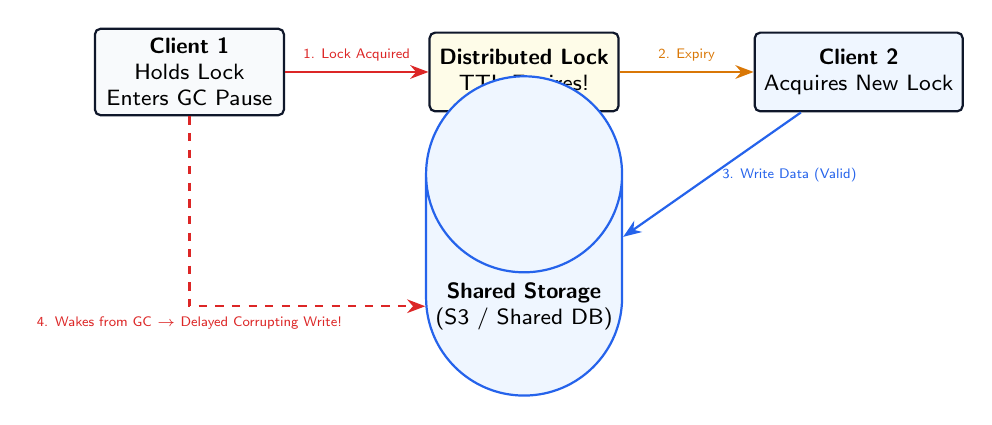
\begin{tikzpicture}[
  scale=0.85,
  box/.style={rectangle, draw=headingblue, fill=codebg, thick, rounded corners=2pt, minimum width=2.4cm, minimum height=1.0cm, align=center, font=\sffamily\footnotesize},
  storage/.style={cylinder, draw=exampleBlue, fill=exampleBg, thick, shape border rotate=90, minimum width=2.2cm, minimum height=1.4cm, align=center, font=\sffamily\footnotesize}
]
  \node[box] (c1) at (0, 2) {\textbf{Client 1}\\Holds Lock\\Enters GC Pause};
  \node[box, fill=mistakeBg] (lock) at (5, 2) {\textbf{Distributed Lock}\\TTL Expires!};
  \node[box, fill=exampleBg] (c2) at (10, 2) {\textbf{Client 2}\\Acquires New Lock};
  \node[storage] (store) at (5, -1.5) {\textbf{Shared Storage}\\(S3 / Shared DB)};

  \draw[-{Stealth[scale=1.0]}, thick, color=warningRed] (c1) -- node[above, font=\sffamily\tiny] {1. Lock Acquired} (lock);
  \draw[-{Stealth[scale=1.0]}, thick, color=mistakeAmber] (lock) -- node[above, font=\sffamily\tiny] {2. Expiry} (c2);
  \draw[-{Stealth[scale=1.0]}, thick, color=exampleBlue] (c2) -- node[right, font=\sffamily\tiny] {3. Write Data (Valid)} (store);
  \draw[-{Stealth[scale=1.0]}, thick, dashed, color=warningRed] (c1) |- node[below, font=\sffamily\tiny] {4. Wakes from GC $\to$ Delayed Corrupting Write!} (store);
\end{tikzpicture}
\caption{The Distributed Lock GC Pause Hazard and Corrupting Write}
\label{fig:gc-pause-hazard}
\end{figure}

Kleppmann identified three inescapable real-world conditions that break Redlock:
\begin{enumerate}[leftmargin=18pt]
  \item \textbf{Process Pauses}: A full JVM garbage collection cycle, SIGSTOP signal, or page fault can pause a client for tens of seconds. During the pause, the lock expires. When the process awakes, it has no awareness that time has passed and executes its mutated write concurrently with another client.
  \item \textbf{Asynchronous Network Latency}: Packets can be delayed arbitrarily in transit.
  \item \textbf{Clock Skew and System Time Steps}: Redlock relies on physical wall-clock elapsed time to determine whether a lease is valid. If NTP steps a node's clock forward, a key can expire instantly before the client uses it.
\end{enumerate}

\section{Fencing Tokens: Storage-Enforced Mutual Exclusion}

Kleppmann demonstrated that a distributed lock service \textbf{cannot guarantee mutual exclusion by itself}. To achieve true safety, the shared storage tier must participate in verification using \textbf{Fencing Tokens}.

\begin{figure}[htbp]
\centering
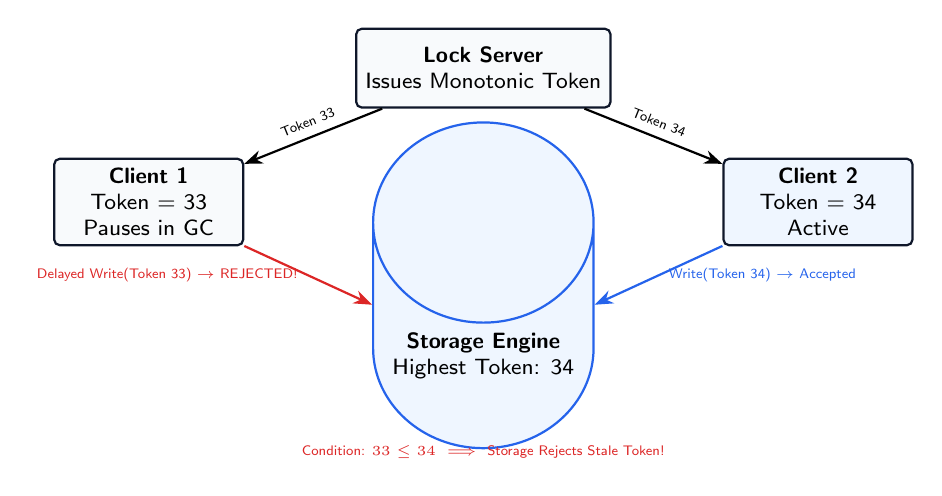
\begin{tikzpicture}[
  scale=0.85,
  box/.style={rectangle, draw=headingblue, fill=codebg, thick, rounded corners=2pt, minimum width=2.4cm, minimum height=1.0cm, align=center, font=\sffamily\footnotesize},
  storage/.style={cylinder, draw=exampleBlue, fill=exampleBg, thick, shape border rotate=90, minimum width=2.8cm, minimum height=1.6cm, align=center, font=\sffamily\footnotesize}
]
  \node[box] (lock) at (5, 2.5) {\textbf{Lock Server}\\Issues Monotonic Token};
  \node[box] (c1) at (0, 0.5) {\textbf{Client 1}\\Token = 33\\Pauses in GC};
  \node[box, fill=exampleBg] (c2) at (10, 0.5) {\textbf{Client 2}\\Token = 34\\Active};
  \node[storage] (store) at (5, -1.8) {\textbf{Storage Engine}\\Highest Token: 34};

  \draw[-{Stealth[scale=1.0]}, thick] (lock) -- node[above, sloped, font=\sffamily\tiny] {Token 33} (c1);
  \draw[-{Stealth[scale=1.0]}, thick] (lock) -- node[above, sloped, font=\sffamily\tiny] {Token 34} (c2);

  \draw[-{Stealth[scale=1.0]}, thick, color=exampleBlue] (c2) -- node[right, font=\sffamily\tiny] {Write(Token 34) $\to$ Accepted} (store);
  \draw[-{Stealth[scale=1.0]}, thick, color=warningRed] (c1) -- node[left, font=\sffamily\tiny] {Delayed Write(Token 33) $\to$ REJECTED!} (store);

  \node[anchor=north, font=\sffamily\tiny, color=warningRed] at (5, -3.0) {Condition: $33 \le 34 \implies$ Storage Rejects Stale Token!};
\end{tikzpicture}
\caption{Fencing Tokens Enforcing Correctness at the Storage Boundary}
\label{fig:fencing-tokens}
\end{figure}

\textbf{Fencing Token Protocol Rules:}
\begin{enumerate}[leftmargin=18pt]
  \item Every time the lock service grants a lock, it increments an atomic counter and returns the value as a fencing token (e.g., Token 33, Token 34).
  \item When a client writes to the database or storage layer, it attaches its fencing token to the write request.
  \item The storage layer maintains the highest token it has ever observed. If a write arrives with a token smaller than or equal to the highest observed token ($Token_{\text{incoming}} \le Token_{\text{max}}$), the storage layer \textbf{rejects the write with an error}.
\end{enumerate}

\begin{lstlisting}[language=SQL, caption={PostgreSQL Storage-Side Fencing Enforcement}]
-- Storage Table with Monotonic Fencing Guard
CREATE TABLE document_storage (
    doc_id VARCHAR(64) PRIMARY KEY,
    payload TEXT NOT NULL,
    fencing_token BIGINT NOT NULL
);

-- Atomic Write guarded by Fencing Token
UPDATE document_storage
SET payload = 'new content from client',
    fencing_token = 34
WHERE doc_id = 'doc_991'
  AND fencing_token < 34; -- Rejects any stale worker with token <= 33
\end{lstlisting}

\section{Database-Native and Consensus Alternatives}

When systems require distributed locking without the operational complexity of Redlock or custom fencing tokens, two proven alternatives exist:

\subsection{PostgreSQL Session Advisory Locks}
PostgreSQL provides application-level locks that do not lock physical rows or tables. Advisory locks operate within the database's internal lock manager and are tied to a database connection session:
\begin{lstlisting}[language=SQL]
-- Non-blocking lock attempt (returns true/false immediately)
SELECT pg_try_advisory_lock(149204);

-- Critical section execution ...

-- Explicit release
SELECT pg_advisory_unlock(149204);
\end{lstlisting}
If the worker crashes or the TCP socket drops, PostgreSQL automatically releases the advisory lock immediately.

\subsection{ZooKeeper / etcd Ephemeral Sequential Nodes}
In Apache ZooKeeper or etcd (which run Raft/ZAB consensus):
\begin{itemize}[leftmargin=18pt]
  \item The client creates an \textbf{ephemeral sequential} znode: \texttt{/locks/resource-00000001}.
  \item An ephemeral node exists only as long as the client's heartbeat session is active. If the client crashes, the consensus cluster deletes the node.
  \item Clients order themselves by sequence number. Client A holds the lock if its sequence number is the lowest in the directory.
  \item Other clients set a \textbf{Watch} on the immediately preceding node, avoiding herd stampedes and waking up sequentially as locks are released.
\end{itemize}

\section{Summary \& Key Takeaways}
\begin{itemize}[leftmargin=18pt]
  \item Distributed locks require leases with TTLs to prevent permanent deadlocks caused by crashed clients.
  \item Redis locks must be released using atomic Lua scripts comparing unique ownership tokens.
  \item Martin Kleppmann proved that distributed locks alone cannot guarantee safety due to GC pauses, asynchronous network delays, and clock jumps.
  \item True safety requires \textbf{Fencing Tokens}: monotonically increasing integers passed to the storage engine, which rejects any write with a token older than the highest observed.
  \item Robust alternatives include PostgreSQL session advisory locks and ZooKeeper/etcd ephemeral sequential znodes.
\end{itemize}

\section{Exercises}

\subsection{Mechanics}
Write an atomic Redis Lua script to extend (heartbeat renew) an existing lock's TTL by 10,000 milliseconds only if the client still owns the lock.

\subsection{Debugging}
A developer writes a distributed lock wrapper in Python:
\begin{lstlisting}[language=Python]
class BadLock:
    def acquire(self, key):
        while not redis.set(key, "1", nx=True):
            time.sleep(0.1)

    def release(self, key):
        redis.delete(key)
\end{lstlisting}
Identify two critical bugs that will lead to catastrophic production failures.

\subsection{Architecture}
You are designing an automated recurring billing engine that executes every night at 02:00 AM across a cluster of 50 Kubernetes pods. Design an end-to-end architecture using PostgreSQL advisory locks and transaction fencing to guarantee that no invoice is charged twice, even during pod rollouts.

\section{Detailed Solutions}

\subsection{Solution to Mechanics Exercise}
\begin{lstlisting}[language=Python]
LUA_RENEW_LOCK = """
if redis.call('get', KEYS[1]) == ARGV[1] then
    return redis.call('pexpire', KEYS[1], ARGV[2])
else
    return 0
end
"""
# Usage: redis.eval(LUA_RENEW_LOCK, 1, "lock:invoice", client_uuid, 10000)
\end{lstlisting}

\subsection{Solution to Debugging Exercise}
\textbf{Critical Bug 1: No TTL / Lease Expiration.}
The call \texttt{redis.set(key, "1", nx=True)} omits an expiration parameter (\texttt{ex} or \texttt{px}). If the worker process encounters a kernel panic, OOM kill, or power failure while holding the lock, the key \texttt{"1"} persists in Redis forever. All other workers will loop infinitely in \texttt{time.sleep(0.1)}, freezing the entire system permanently.
\textbf{Critical Bug 2: Blind Lock Deletion.}
In \texttt{release()}, the code executes \texttt{redis.delete(key)}. Because the stored value is a static \texttt{"1"} rather than a unique UUID, any worker can inadvertently delete a lock held by a different worker.

\subsection{Solution to Architecture Exercise}
\textbf{Architecture:}
\begin{enumerate}[leftmargin=18pt]
  \item \textbf{Global Leader Election via Advisory Lock}: A worker pod attempts to acquire a cluster-wide leader lock using PostgreSQL:
  \begin{lstlisting}[language=SQL]
  SELECT pg_try_advisory_lock(hashtext('daily_billing_job_2026_11_23'));
  \end{lstlisting}
  If the function returns \texttt{false}, the pod immediately terminates and waits for tomorrow's schedule. Only one pod becomes the billing orchestrator.
  \item \textbf{Row-Level Invoice Fencing}: The leader queries unprocessed invoices and processes them in batches. To prevent concurrent worker collisions or mid-job pod restarts, each invoice update utilizes an optimistic concurrency version column and status transition:
  \begin{lstlisting}[language=SQL]
  UPDATE invoices
  SET status = 'PROCESSING',
      lock_version = lock_version + 1,
      locked_by = 'pod_worker_7a'
  WHERE id = :invoice_id
    AND status = 'PENDING'
    AND lock_version = :expected_version;
  \end{lstlisting}
  If \texttt{rowcount == 0}, the invoice was already claimed.
  \item \textbf{Idempotent Payment Execution}: Pass \texttt{invoice\_id || '\_' || lock\_version} to Stripe as the payment idempotency key.
\end{enumerate}

\section{Further Reading \& Citations}
\begin{itemize}[leftmargin=18pt]
  \item Kleppmann, M. (2016). \emph{How to do distributed locking}. Available at \url{https://martin.kleppmann.com/2016/02/08/how-to-do-distributed-locking.html}.
  \item Sanfilippo, S. (2016). \emph{Is Redlock safe?}. Available at \url{http://antirez.com/news/101}.
  \item Hunt, P., et al. (2010). \emph{ZooKeeper: Wait-free coordination for large distributed systems}. In USENIX Annual Technical Conference (ATC 10), 145--158.
\end{itemize}

\chapter{Sagas, CQRS, and Event Sourcing}
\label{ch:sagas-cqrs-eventsourcing}

\begin{chaptergoalsbox}
\textbf{What you will learn:}
\begin{itemize}[leftmargin=12pt]
  \item The Dual-Write Problem: why updating a database and publishing an event to a message broker in separate steps guarantees state corruption.
  \item The Transactional Outbox Pattern: achieving guaranteed message delivery using local ACID transactions and Change Data Capture (CDC via Debezium).
  \item The Saga Pattern: managing long-running distributed business transactions via local transactions and compensating actions.
  \item Saga Topologies: Orchestrated Sagas (centralized state machines) vs. Choreographed Sagas (decentralized event gossip).
  \item Command Query Responsibility Segregation (CQRS): separating write models (aggregates) from read models (denormalized query projections).
  \item Event Sourcing: modeling application state as an append-only stream of immutable domain events, snapshotting, and projection rebuilds.
\end{itemize}

\textbf{What you should already understand:}
\begin{itemize}[leftmargin=12pt]
  \item Database write-ahead logging (WAL) and local ACID transaction semantics.
  \item Messaging brokers (Kafka/RabbitMQ) and at-least-once delivery from Chapter~\ref{ch:messaging-systems} and Chapter~\ref{ch:kafka-rabbitmq}.
\end{itemize}

\textbf{Why this topic exists:}
Because Two-Phase Commit (2PC) is slow, blocking, and unsupported across polyglot microservice boundaries, distributed architectures must embrace eventual consistency. Sagas, CQRS, and Event Sourcing provide mathematically sound patterns to coordinate business state across independent microservices.

\textbf{Motivating practical problem:}
An e-commerce order service executes: \texttt{db.saveOrder()} followed by \texttt{kafka.send("order\_created")}. After saving the order to PostgreSQL, the pod is killed by Kubernetes due to a memory limit. The order is stored in the database, but the event is never published. The payment service and warehouse packing service never receive the notification; the customer is never charged, the order is never shipped, and the system enters an undetectable ghost state.
\end{chaptergoalsbox}

\section{The Dual-Write Problem}

In a microservices architecture, operations frequently require updating an internal database and publishing an event to an external broker:

\begin{lstlisting}[language=Python, caption={The Flawed Dual-Write Anti-Pattern}]
def create_order(order_data):
    # Step 1: Write to local relational database
    db.orders.insert(order_data)

    # Step 2: Publish event to Kafka
    kafka_producer.send("order_events", order_data)
\end{lstlisting}

\begin{productionwarningbox}[The Inescapable Dual-Write Failure States]
No matter which order you arrange Step 1 and Step 2, failure is guaranteed:
\begin{itemize}[leftmargin=12pt]
  \item \textbf{DB First, then Kafka}: If the application server crashes, network partitions hit Kafka, or the JVM pauses between Step 1 and Step 2, the DB transaction commits but the event is never dispatched. The rest of the distributed system is unaware the order exists.
  \item \textbf{Kafka First, then DB}: If the Kafka send succeeds, but the database insertion fails due to a unique key collision or disk full error, consumers begin fulfilling an order that does not exist in the database.
\end{itemize}
Because the database and the Kafka broker are separate distributed systems that do not share an atomic commit protocol, executing dual writes directly in application code violates Atomicity.
\end{productionwarningbox}

\section{The Transactional Outbox Pattern and CDC}

The \textbf{Transactional Outbox Pattern} solves the dual-write problem by leveraging the database's local ACID transaction guarantee.

\begin{figure}[htbp]
\centering
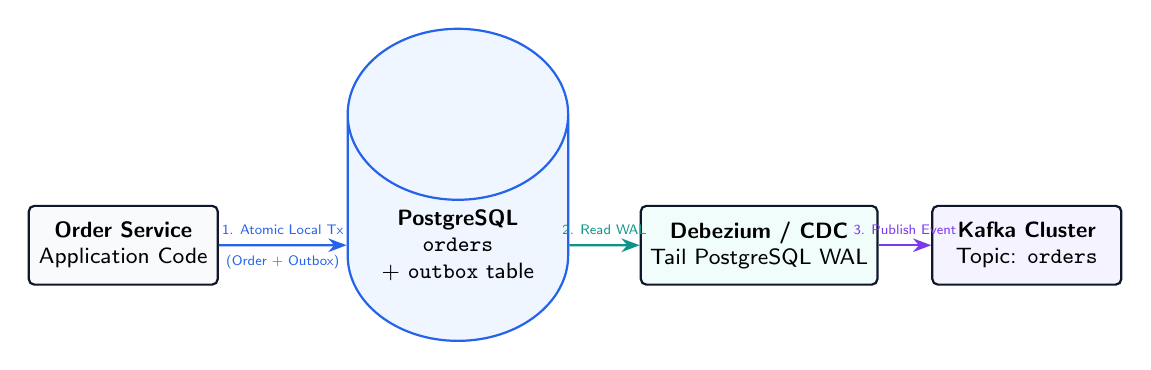
\begin{tikzpicture}[
  scale=0.85,
  box/.style={rectangle, draw=headingblue, fill=codebg, thick, rounded corners=2pt, minimum width=2.4cm, minimum height=1.0cm, align=center, font=\sffamily\footnotesize},
  db/.style={cylinder, draw=exampleBlue, fill=exampleBg, thick, shape border rotate=90, minimum width=2.8cm, minimum height=1.8cm, align=center, font=\sffamily\footnotesize}
]
  \node[box] (app) at (0, 0) {\textbf{Order Service}\\Application Code};
  \node[db] (db) at (5, 0) {\textbf{PostgreSQL}\\\texttt{orders}\\+ \texttt{outbox} table};
  \node[box, fill=intuitionBg] (cdc) at (9.5, 0) {\textbf{Debezium / CDC}\\Tail PostgreSQL WAL};
  \node[box, fill=tryBg] (kafka) at (13.5, 0) {\textbf{Kafka Cluster}\\Topic: \texttt{orders}};

  \draw[-{Stealth[scale=1.0]}, thick, color=exampleBlue] (app) -- node[above, font=\sffamily\tiny] {1. Atomic Local Tx} node[below, font=\sffamily\tiny] {(Order + Outbox)} (db);
  \draw[-{Stealth[scale=1.0]}, thick, color=intuitionTeal] (db) -- node[above, font=\sffamily\tiny] {2. Read WAL} (cdc);
  \draw[-{Stealth[scale=1.0]}, thick, color=tryViolet] (cdc) -- node[above, font=\sffamily\tiny] {3. Publish Event} (kafka);
\end{tikzpicture}
\caption{The Transactional Outbox Pattern with Change Data Capture (Debezium)}
\label{fig:outbox-pattern}
\end{figure}

\subsection{Implementation Mechanics}

\begin{enumerate}[leftmargin=18pt]
  \item \textbf{The Outbox Table}: A dedicated table is added to the application database:
  \begin{lstlisting}[language=SQL]
  CREATE TABLE outbox_events (
      id UUID PRIMARY KEY DEFAULT gen_random_uuid(),
      aggregate_type VARCHAR(64) NOT NULL,
      aggregate_id VARCHAR(64) NOT NULL,
      event_type VARCHAR(64) NOT NULL,
      payload JSONB NOT NULL,
      created_at TIMESTAMPTZ NOT NULL DEFAULT NOW()
  );
  \end{lstlisting}
  \item \textbf{Atomic Local Write}: When an order is created, the service inserts both the business entity into \texttt{orders} and the event record into \texttt{outbox\_events} within the \textbf{same single database transaction}:
  \begin{lstlisting}[language=SQL]
  BEGIN;
  INSERT INTO orders (id, customer_id, total) VALUES ('ord_1', 'cust_9', 99.00);
  INSERT INTO outbox_events (aggregate_type, aggregate_id, event_type, payload)
  VALUES ('Order', 'ord_1', 'OrderCreated', '{"total": 99.00}');
  COMMIT;
  \end{lstlisting}
  \item \textbf{Asynchronous Relay}: A relay process reads records from \texttt{outbox\_events} and publishes them to Kafka.
  \begin{itemize}[leftmargin=12pt]
    \item \textbf{Polling Publisher}: A background worker runs \texttt{SELECT ... FOR UPDATE SKIP LOCKED} every $500\text{ ms}$, publishes to Kafka, and deletes the processed rows. (High polling overhead).
    \item \textbf{Change Data Capture (CDC via Debezium)}: Debezium connects directly to the PostgreSQL logical replication stream (reading the binary Write-Ahead Log). As soon as the transaction commits to disk, Debezium streams the outbox insert straight into Kafka with sub-millisecond latency and zero polling CPU load.
  \end{itemize}
\end{enumerate}

\section{The Saga Pattern}

In 1987, Hector Garcia-Molina and Kenneth Salem formulated the \textbf{Saga Pattern}. A Saga is an architectural mechanism to execute long-running transactions across multiple independent databases without distributed locks.

A Saga breaks a distributed transaction into a sequence of $N$ local transactions: $T_1, T_2, \dots, T_n$. Each local transaction $T_i$ updates state within a single service and commits. If any transaction $T_k$ fails (e.g., credit check fails or out of stock), the saga executes a series of \textbf{Compensating Transactions} $C_{k-1}, \dots, C_1$ in reverse order to undo the changes made by preceding steps.

\begin{figure}[htbp]
\centering
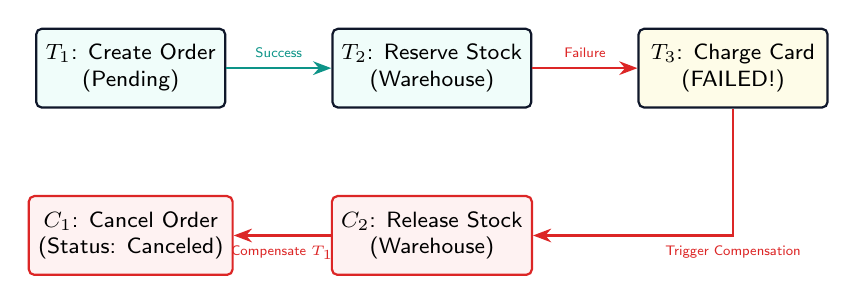
\begin{tikzpicture}[
  scale=0.85,
  tx/.style={rectangle, draw=headingblue, fill=codebg, thick, rounded corners=2pt, minimum width=2.4cm, minimum height=1.0cm, align=center, font=\sffamily\footnotesize},
  comp/.style={rectangle, draw=warningRed, fill=warningBg, thick, rounded corners=2pt, minimum width=2.4cm, minimum height=1.0cm, align=center, font=\sffamily\footnotesize}
]
  \node[tx, fill=intuitionBg] (t1) at (0, 1.5) {$T_1$: Create Order\\(Pending)};
  \node[tx, fill=intuitionBg] (t2) at (4.5, 1.5) {$T_2$: Reserve Stock\\(Warehouse)};
  \node[tx, fill=mistakeBg] (t3) at (9, 1.5) {$T_3$: Charge Card\\(FAILED!)};

  \node[comp] (c2) at (4.5, -1.0) {$C_2$: Release Stock\\(Warehouse)};
  \node[comp] (c1) at (0, -1.0) {$C_1$: Cancel Order\\(Status: Canceled)};

  \draw[-{Stealth[scale=1.0]}, thick, color=intuitionTeal] (t1) -- node[above, font=\sffamily\tiny] {Success} (t2);
  \draw[-{Stealth[scale=1.0]}, thick, color=warningRed] (t2) -- node[above, font=\sffamily\tiny] {Failure} (t3);

  \draw[-{Stealth[scale=1.0]}, thick, color=warningRed] (t3) |- node[below, font=\sffamily\tiny] {Trigger Compensation} (c2);
  \draw[-{Stealth[scale=1.0]}, thick, color=warningRed] (c2) -- node[below, font=\sffamily\tiny] {Compensate $T_1$} (c1);
\end{tikzpicture}
\caption{Saga Execution Flow with Reverse Compensating Transactions}
\label{fig:saga-flow}
\end{figure}

\begin{intuitionbox}[Semantic Compensation vs. Physical Rollback]
A database rollback physically restores bits on disk to their pre-transaction values, as if the transaction never occurred. A Saga \textbf{cannot} physically roll back because previous local transactions have already committed and their changes were made visible to other users.
A compensating transaction is a \textbf{semantic counter-action}:
\begin{itemize}[leftmargin=12pt]
  \item If $T_1$ credited \$100 to an account, $C_1$ debits \$100.
  \item If $T_2$ reserved 3 seats on a flight, $C_2$ releases the 3 seats.
  \item If $T_3$ sent an email confirmation, $C_3$ sends an apology email explaining the order cancellation.
\end{itemize}
\end{intuitionbox}

\subsection{Orchestration vs. Choreography}

\begin{table}[htbp]
\centering\small
\begin{tabular}{lp{5.5cm}p{5.5cm}}
\toprule
\textbf{Dimension} & \textbf{Choreography (Decentralized)} & \textbf{Orchestration (Centralized)} \\
\midrule
\textbf{Coordination} & Services listen to events and autonomously decide when to execute local steps and publish next events. & A dedicated state machine (Orchestrator) sends explicit commands to services and tracks progress. \\
\textbf{Coupling} & Low spatial coupling. Services do not know about each other. & Moderate coupling. Services must implement API/command contracts defined by the orchestrator. \\
\textbf{Visibility} & Poor. Distributed state transitions are spread across multiple logs; difficult to determine where a saga stalled. & Excellent. The central orchestrator logs the complete execution graph, state history, and timeouts in one place. \\
\textbf{Complexity} & High risk of circular event storms and cyclic dependencies as business flows scale beyond 4 steps. & Scales cleanly to dozens of steps. Built using tools like Temporal.io, AWS Step Functions, or Camunda. \\
\bottomrule
\end{tabular}
\caption{Architectural Comparison: Choreographed vs. Orchestrated Sagas}
\label{tab:saga-comparison}
\end{table}

\section{Command Query Responsibility Segregation (CQRS)}

Traditional relational applications use a single data model for both reads and writes. As systems scale, this creates conflicting pressures: write operations require normalized 3NF schemas to prevent update anomalies and ensure lock efficiency, whereas complex UI queries require highly denormalized joins, full-text indexing, and aggregation.

\textbf{CQRS} (formulated by Greg Young and Bertrand Meyer) separates the application into two distinct paths:
\begin{enumerate}[leftmargin=18pt]
  \item \textbf{Command Side (Write Model)}: Handles business validation, invariants, and transactional mutations. Optimized strictly for consistency and write throughput. Emits domain events.
  \item \textbf{Query Side (Read Model)}: Consumes domain events and projects them into read-optimized data stores (e.g., Elasticsearch for search, Redis for caching, PostgreSQL denormalized views for dashboards). Completely read-only.
\end{enumerate}

\begin{figure}[htbp]
\centering
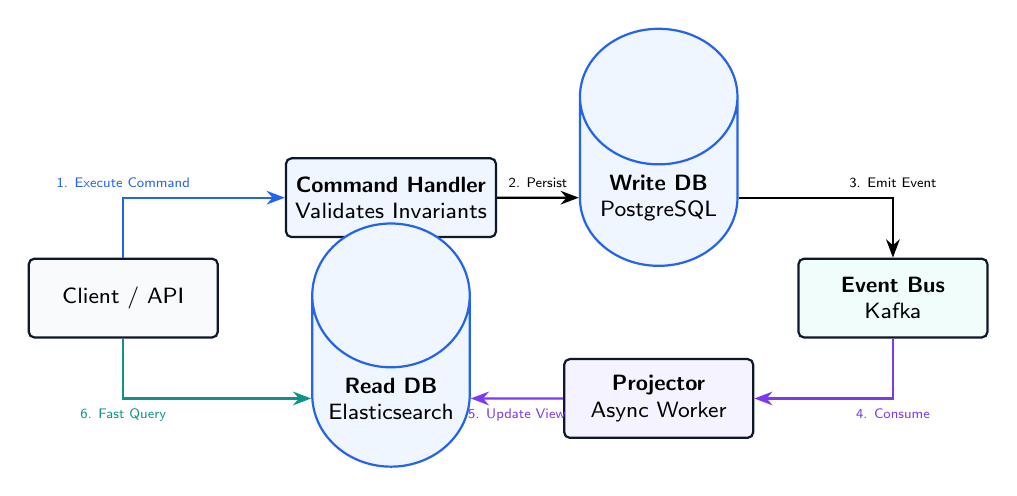
\begin{tikzpicture}[
  scale=0.85,
  box/.style={rectangle, draw=headingblue, fill=codebg, thick, rounded corners=2pt, minimum width=2.4cm, minimum height=1.0cm, align=center, font=\sffamily\footnotesize},
  db/.style={cylinder, draw=exampleBlue, fill=exampleBg, thick, shape border rotate=90, minimum width=2.0cm, minimum height=1.4cm, align=center, font=\sffamily\footnotesize}
]
  \node[box] (client) at (0, 0) {Client / API};
  \node[box, fill=exampleBg] (cmd) at (4, 1.5) {\textbf{Command Handler}\\Validates Invariants};
  \node[db] (write_db) at (8, 1.5) {\textbf{Write DB}\\PostgreSQL};
  \node[box, fill=intuitionBg] (bus) at (11.5, 0) {\textbf{Event Bus}\\Kafka};
  \node[box, fill=tryBg] (proj) at (8, -1.5) {\textbf{Projector}\\Async Worker};
  \node[db] (read_db) at (4, -1.5) {\textbf{Read DB}\\Elasticsearch};

  \draw[-{Stealth[scale=1.0]}, thick, color=exampleBlue] (client) |- node[above, font=\sffamily\tiny] {1. Execute Command} (cmd);
  \draw[-{Stealth[scale=1.0]}, thick] (cmd) -- node[above, font=\sffamily\tiny] {2. Persist} (write_db);
  \draw[-{Stealth[scale=1.0]}, thick] (write_db) -| node[above, font=\sffamily\tiny] {3. Emit Event} (bus);
  \draw[-{Stealth[scale=1.0]}, thick, color=tryViolet] (bus) |- node[below, font=\sffamily\tiny] {4. Consume} (proj);
  \draw[-{Stealth[scale=1.0]}, thick, color=tryViolet] (proj) -- node[below, font=\sffamily\tiny] {5. Update View} (read_db);
  \draw[-{Stealth[scale=1.0]}, thick, color=intuitionTeal] (client) |- node[below, font=\sffamily\tiny] {6. Fast Query} (read_db);
\end{tikzpicture}
\caption{CQRS Architectural Flow: Decoupled Write and Read Projections}
\label{fig:cqrs-architecture}
\end{figure}

\section{Event Sourcing}

In traditional state-oriented systems (CRUD), the database stores only the \textbf{current state} of an entity. When an address changes, an \texttt{UPDATE} statement overwrites the old address, destroying historical context.

In \textbf{Event Sourcing}, application state is modeled as an append-only stream of immutable domain events. The database is called an \textbf{Event Store}.

\subsection{State Reconstruction and Projections}

Current state is never stored directly; it is calculated at runtime by \textbf{replaying} events from the beginning of time:
\begin{equation}
\text{State}_N = \text{FoldLeft}(\text{InitialState}, [E_1, E_2, \dots, E_N])
\end{equation}

\begin{lstlisting}[language=Python, caption={Event Sourcing Domain Aggregate in Python}]
from typing import List

class BankAccountAggregate:
    def __init__(self, account_id: str):
        self.account_id = account_id
        self.balance = 0.0
        self.is_closed = False
        self.version = 0

    def apply_event(self, event: dict):
        """Mutates internal aggregate state deterministically."""
        event_type = event["type"]
        if event_type == "AccountOpened":
            self.balance = event["initial_balance"]
        elif event_type == "FundsDeposited":
            self.balance += event["amount"]
        elif event_type == "FundsWithdrawn":
            self.balance -= event["amount"]
        elif event_type == "AccountClosed":
            self.is_closed = True
        self.version = event["version"]

    def replay_events(self, history: List[dict]):
        for event in history:
            self.apply_event(event)

    # Command Handling with Invariant Validation
    def withdraw(self, amount: float) -> dict:
        if self.is_closed:
            raise ValueError("Account is closed.")
        if amount > self.balance:
            raise ValueError("Insufficient funds.")

        # Emits a new immutable event
        return {
            "type": "FundsWithdrawn",
            "account_id": self.account_id,
            "amount": amount,
            "version": self.version + 1
        }
\end{lstlisting}

\begin{underthehoodbox}[Snapshotting Performance Optimization]
If an aggregate has 50,000 historical events, replaying the entire stream on every read operation would take hundreds of milliseconds.
To optimize recovery, systems take periodic \textbf{Snapshots} (e.g., every 100 events). A snapshot serializes the exact state at version $K$. When loading, the engine loads Snapshot $K$ and only replays events from $K+1$ to $N$.
\end{underthehoodbox}

\section{Summary \& Key Takeaways}
\begin{itemize}[leftmargin=18pt]
  \item Dual-writes directly in application code violate distributed atomicity because partial failures leave databases and message brokers permanently desynchronized.
  \item The Transactional Outbox pattern guarantees at-least-once message publication by writing domain state and outbox events within the same local ACID transaction, dispatched asynchronously via Change Data Capture (Debezium).
  \item Sagas replace blocking 2PC transactions across microservices using a sequence of local transactions paired with reverse compensating actions.
  \item Orchestrated sagas use centralized state machines (Temporal, Step Functions) to provide comprehensive observability and eliminate cyclic event deadlocks.
  \item CQRS separates command write models from read-optimized query projections, decoupling transactional constraints from complex user queries.
  \item Event Sourcing stores the sequence of immutable domain events as the authoritative system of record, deriving current state via deterministic replay and periodic snapshotting.
\end{itemize}

\section{Exercises}

\subsection{Mechanics}
Write an event sourcing stream for a customer shopping cart:
\begin{enumerate}[leftmargin=18pt]
  \item Emitting events: \texttt{CartCreated}, \texttt{ItemAdded(SKU123, qty=2)}, \texttt{ItemAdded(SKU456, qty=1)}, \texttt{ItemRemoved(SKU123, qty=1)}.
  \item Demonstrate the mathematical fold function that derives the final shopping cart contents.
\end{enumerate}

\subsection{Debugging}
A microservice architecture uses a choreographed saga for ride-sharing bookings. Service A publishes \texttt{RideRequested}; Service B listens and reserves a driver, publishing \texttt{DriverReserved}; Service C listens and attempts to charge the rider's credit card. If Service C fails, it publishes \texttt{PaymentFailed}.
During testing, engineers observe that when a payment fails, Service B releases the driver, but Service A receives \texttt{DriverReleased} and incorrectly triggers another \texttt{RideRequested} event, entering an infinite loop. Explain how to break this cyclic dependency.

\subsection{Architecture}
Architect an event-sourced cryptocurrency exchange ledger. Detail:
\begin{enumerate}[leftmargin=18pt]
  \item The Event Store PostgreSQL schema supporting optimistic concurrency control (handling concurrent deposits/withdrawals).
  \item The Kafka outbox pipeline streaming events to real-time CQRS projections (account balance cache in Redis, audit history in ClickHouse).
\end{enumerate}

\section{Detailed Solutions}

\subsection{Solution to Mechanics Exercise}
\begin{lstlisting}[language=Python]
events = [
    {"type": "CartCreated", "cart_id": "c1"},
    {"type": "ItemAdded", "sku": "SKU123", "qty": 2},
    {"type": "ItemAdded", "sku": "SKU456", "qty": 1},
    {"type": "ItemRemoved", "sku": "SKU123", "qty": 1}
]

def reduce_cart(cart: dict, event: dict) -> dict:
    etype = event["type"]
    if etype == "ItemAdded":
        sku, qty = event["sku"], event["qty"]
        cart[sku] = cart.get(sku, 0) + qty
    elif etype == "ItemRemoved":
        sku, qty = event["sku"], event["qty"]
        cart[sku] = max(0, cart.get(sku, 0) - qty)
        if cart[sku] == 0:
            del cart[sku]
    return cart

final_state = functools.reduce(reduce_cart, events, {})
# Output: {'SKU123': 1, 'SKU456': 1}
\end{lstlisting}

\subsection{Solution to Debugging Exercise}
\textbf{The Cyclic Event Storm Root Cause:}
In choreographed sagas, services listen to generic domain events rather than targeted commands. When Service A treats \texttt{DriverReleased} as an indicator to retry a ride request, it conflates a normal compensation state with a new request.
\textbf{Architectural Mitigations:}
1. \textbf{Correlation \& Saga IDs}: Every saga must carry a unique \texttt{saga\_id}. Service A must check the saga's current lifecycle state. If \texttt{saga.status == CANCELED}, ignore downstream compensation events.
2. \textbf{Explicit Event Semantics}: Differentiate between \emph{Domain Events} (\texttt{DriverWasReleased}) and \emph{Compensation Completed Events} (\texttt{RideBookingFailedAndCleanedUp}).
3. \textbf{Migrate to Orchestration}: Replace decentralized choreography with a central orchestrator (like Temporal). The orchestrator explicitly commands: \texttt{ReleaseDriver(saga\_id)}, waits for acknowledgment, transitions the state to \texttt{FAILED}, and stops without firing cyclic events.

\subsection{Solution to Architecture Exercise}
\textbf{Event Store Schema with Optimistic Concurrency Control:}
\begin{lstlisting}[language=SQL]
CREATE TABLE event_store (
    stream_id UUID NOT NULL,
    version BIGINT NOT NULL,
    event_type VARCHAR(64) NOT NULL,
    payload JSONB NOT NULL,
    created_at TIMESTAMPTZ NOT NULL DEFAULT NOW(),
    PRIMARY KEY (stream_id, version) -- Guarantees optimistic concurrency!
);
\end{lstlisting}
When appending an event, the application specifies the expected previous version:
\begin{lstlisting}[language=SQL]
-- Append event for account_id with expected version 4
INSERT INTO event_store (stream_id, version, event_type, payload)
VALUES ('748e-acc', 5, 'FundsWithdrawn', '{"amount": 500.00}');
\end{lstlisting}
If two concurrent transactions attempt to append version 5, PostgreSQL's primary key constraint causes one to immediately fail with a unique violation, preventing double-spend race conditions.

\textbf{Outbox \& CQRS Pipeline:}
\begin{enumerate}[leftmargin=18pt]
  \item Debezium tails \texttt{event\_store} WAL commits and writes events to Kafka topic \texttt{exchange.events} partitioned by \texttt{stream\_id}.
  \item \textbf{Redis Projection Worker}: Reads stream sequentially, updating \texttt{HSET account:\{id\} balance \$new\_balance}.
  \item \textbf{ClickHouse Projector}: Batches events into ClickHouse columnar storage for real-time compliance reporting.
\end{enumerate}

\section{Further Reading \& Citations}
\begin{itemize}[leftmargin=18pt]
  \item Garcia-Molina, H., \& Salem, K. (1987). \emph{Sagas}. ACM SIGMOD Record, 16(3), 249--259.
  \item Young, G. (2010). \emph{CQRS Documents}. Available at \url{https://cqrs.files.wordpress.com/2010/11/cqrs_documents.pdf}.
  \item Richardson, C. (2018). \emph{Microservices Patterns: With examples in Java}. Manning Publications.
  \item Fowler, M. (2005). \emph{Event Sourcing}. Available at \url{https://martinfowler.com/eaaDev/EventSourcing.html}.
\end{itemize}

\chapter{Reliability and Fault Tolerance}
\label{ch:reliability-fault-tolerance}

\begin{chaptergoalsbox}
\textbf{What you will learn:}
\begin{itemize}[leftmargin=12pt]
  \item Accrual failure detection: the $\varphi$-Accrual Failure Detector algorithm (Hayashibara et al.) and adaptive heartbeat windows.
  \item Cascading failures: the dynamics of retry storms, amplification factors, and why fixed-interval retries destroy struggling dependencies.
  \item Exponential backoff with Full Jitter: mathematical derivation (AWS Architecture research) and collision avoidance.
  \item Protective isolation patterns: Michael Nygard's Circuit Breaker state machine (Closed, Open, Half-Open) and Bulkheads (thread pool / concurrency isolation).
  \item Load shedding, priority queue shedding, and token-bucket concurrency limits (Little's Law).
  \item Chaos Engineering: Netflix Chaos Monkey principles, failure injection testing, game days, and steady-state hypothesis validation.
\end{itemize}

\textbf{What you should already understand:}
\begin{itemize}[leftmargin=12pt]
  \item Network latency, jitter, and partial failure models from Chapter~\ref{ch:distributed-fundamentals}.
  \item HTTP error status codes, connection pooling, and worker thread pools.
\end{itemize}

\textbf{Why this topic exists:}
At scale, hardware components, network links, and dependent microservices fail constantly. Systems cannot be designed under the fantasy that failures will not occur. Reliability engineering provides mathematical and architectural mechanisms to survive partial degradations without catastrophic total system collapse.

\textbf{Motivating practical problem:}
A critical authentication microservice experiences a minor 500-millisecond database lock spike. Upstream API gateways immediately retry all timed-out requests 3 times with zero delay. Within 3 seconds, traffic volume quadruples from 10,000 QPS to 40,000 QPS. The database connection pool is crushed, the authentication service crashes from out-of-memory errors, and all 15 dependent microservices across the entire enterprise collapse in a cascading outage.
\end{chaptergoalsbox}

\section[Failure Detection: The Phi-Accrual Detector]{Failure Detection: The $\phi$-Accrual Detector}

In distributed systems, traditional failure detectors use a binary threshold: if no heartbeat is received within $\Delta t$ seconds, the target node is declared dead.
\begin{itemize}[leftmargin=18pt]
  \item \textbf{Small Threshold}: Rapid detection, but false positives triggered by transient network jitter or brief GC pauses cause unnecessary, disruptive leader elections.
  \item \textbf{Large Threshold}: High accuracy, but crashes take tens of seconds to detect, stalling traffic.
\end{itemize}

\subsection{Mathematical Formulation}

In 2004, Naohiro Hayashibara et al. introduced the \textbf{$\varphi$-Accrual Failure Detector} (utilized in Apache Cassandra and Akka):

Instead of outputting a binary decision (dead or alive), the detector outputs a continuous suspicion value, $\varphi$ (phi), representing the probability that the monitored node has crashed.

Let the intervals between consecutive heartbeats follow a normal distribution with mean $\mu$ and variance $\sigma^2$, estimated from a sliding window of recent heartbeats.
Given elapsed time $t$ since the last received heartbeat, the probability $P_{\text{later}}(t)$ that a heartbeat will arrive more than $t$ time units after the previous one is:

\begin{equation}
P_{\text{later}}(t) = \frac{1}{\sigma \sqrt{2\pi}} \int_t^\infty e^{-\frac{(x - \mu)^2}{2\sigma^2}} dx
\end{equation}

The suspicion scale $\varphi$ is defined logarithmically:
\begin{equation}
\varphi = -\log_{10}(P_{\text{later}}(t))
\end{equation}

\begin{table}[htbp]
\centering\small
\begin{tabular}{llp{7.5cm}}
\toprule
\textbf{Value of $\varphi$} & \textbf{Probability $P_{\text{later}}(t)$} & \textbf{Interpretation and Action} \\
\midrule
$\varphi = 1$ & $P = 0.1$ ($10\%$) & Normal network jitter; continue waiting. \\
$\varphi = 2$ & $P = 0.01$ ($1\%$) & Suspicious delay; slow down request dispatch to this replica. \\
$\varphi = 3$ & $P = 0.001$ ($0.1\%$) & High suspicion; begin preparing standby replica. \\
$\varphi \ge 8$ & $P \le 10^{-8}$ & Node virtually certain to have crashed; trigger failover and cluster rebalance. \\
\bottomrule
\end{tabular}
\caption{Interpretation of $\varphi$ Suspicion Values in Accrual Failure Detection}
\label{tab:phi-interpretation}
\end{table}

\begin{lstlisting}[language=Python, caption={Python Implementation of a $\varphi$-Accrual Failure Detector}]
import math
import time
from collections import deque

class PhiAccrualFailureDetector:
    def __init__(self, threshold: float = 8.0, max_sample_size: int = 1000):
        self.threshold = threshold
        self.max_sample_size = max_sample_size
        self.intervals = deque(maxlen=max_sample_size)
        self.last_heartbeat_time = None

    def record_heartbeat(self, now: float = None):
        now = now or time.time()
        if self.last_heartbeat_time is not None:
            interval = now - self.last_heartbeat_time
            self.intervals.append(interval)
        self.last_heartbeat_time = now

    def phi(self, now: float = None) -> float:
        if self.last_heartbeat_time is None or len(self.intervals) < 2:
            return 0.0

        now = now or time.time()
        elapsed = now - self.last_heartbeat_time

        # Calculate mean and standard deviation
        mean = sum(self.intervals) / len(self.intervals)
        variance = sum((x - mean) ** 2 for x in self.intervals) / len(self.intervals)
        std_dev = math.sqrt(variance) if variance > 1e-6 else 1e-3

        # Compute cumulative distribution function (CDF) using error function
        y = (elapsed - mean) / (std_dev * math.sqrt(2))
        p_later = 0.5 * (1.0 - math.erf(y))

        if p_later <= 0.0:
            return float('inf')

        return -math.log10(p_later)

    def is_available(self, now: float = None) -> bool:
        return self.phi(now) < self.threshold
\end{lstlisting}

\section{Retry Storms and Exponential Backoff with Jitter}

When a downstream service degrades or experiences transient packet drops, naive client retry behavior is the primary catalyst converting minor slowdowns into catastrophic cluster outages.

\subsection{The Math of Retry Amplification}

Consider a client pipeline making 1,000 QPS to a downstream service. If the downstream service encounters a slowdown that causes 20\% of requests to time out, and clients immediately retry up to 3 times without delay:
\begin{equation}
\text{Total Traffic} = 1{,}000 + (0.20 \times 1{,}000) + (0.20^2 \times 1{,}000) + \dots \approx 1{,}250\text{ QPS}
\end{equation}
If the timeout rate rises to 60\%, the incoming load explodes:
\begin{equation}
\text{Total Traffic} = 1{,}000 \times \sum_{k=0}^{3} (0.6)^k = 1{,}000 \times (1 + 0.6 + 0.36 + 0.216) = 2{,}176\text{ QPS}
\end{equation}
The struggling service, which could not handle 1,000 QPS, is now bombarded with 2,176 QPS. This positive feedback loop is a \textbf{Retry Storm}.

\subsection{Full Jitter Algorithm (AWS Research)}

Marc Brooker et al. at AWS proved that exponential backoff alone is insufficient because all clients retry in synchronized waves (the thundering herd). Adding randomness (\textbf{Jitter}) breaks synchronization.

\begin{figure}[htbp]
\centering
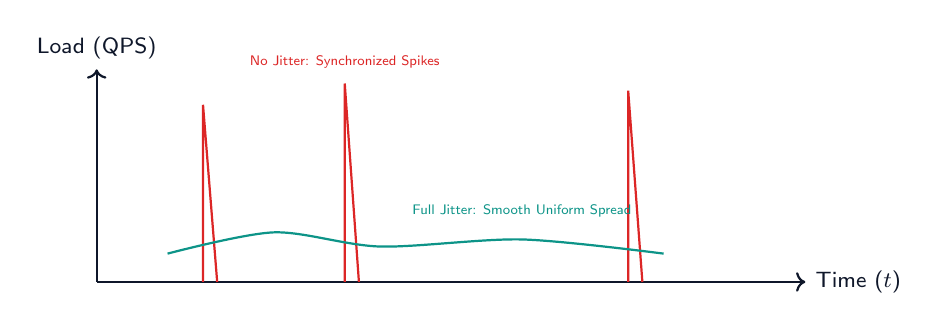
\begin{tikzpicture}[
  scale=0.9,
  axis/.style={->, thick, color=headingblue},
  wave/.style={thick, color=warningRed},
  jitterwave/.style={thick, color=intuitionTeal}
]
  \draw[axis] (0, 0) -- (10, 0) node[right, font=\sffamily\footnotesize] {Time ($t$)};
  \draw[axis] (0, 0) -- (0, 3) node[above, font=\sffamily\footnotesize] {Load (QPS)};

  % No jitter spikes
  \draw[wave] (1.5, 0) -- (1.5, 2.5) -- (1.7, 0);
  \draw[wave] (3.5, 0) -- (3.5, 2.8) -- (3.7, 0);
  \draw[wave] (7.5, 0) -- (7.5, 2.7) -- (7.7, 0);
  \node[font=\sffamily\tiny, color=warningRed] at (3.5, 3.1) {No Jitter: Synchronized Spikes};

  % Full jitter distribution
  \draw[jitterwave, smooth] plot coordinates {(1.0, 0.4) (2.5, 0.7) (4.0, 0.5) (6.0, 0.6) (8.0, 0.4)};
  \node[font=\sffamily\tiny, color=intuitionTeal] at (6.0, 1.0) {Full Jitter: Smooth Uniform Spread};
\end{tikzpicture}
\caption{Traffic Distribution: Synchronized Retry Spikes vs. Smooth Full Jitter}
\label{fig:full-jitter}
\end{figure}

AWS evaluated three jitter algorithms:
\begin{enumerate}[leftmargin=18pt]
  \item \textbf{Equal Jitter}: $t = \frac{\text{temp}}{2} + \text{rand}(0, \frac{\text{temp}}{2})$
  \item \textbf{Decorrelated Jitter}: $t = \min(\text{cap}, \text{rand}(\text{base}, t_{\text{prev}} \times 3))$
  \item \textbf{Full Jitter (Recommended)}:
  \begin{equation}
  \text{sleep} = \text{rand}\left(0, \min\left(\text{Cap}, \text{Base} \times 2^{\text{attempt}}\right)\right)
  \end{equation}
\end{enumerate}
Full Jitter uniformly distributes retries across the entire interval from 0 to the exponential ceiling, yielding the lowest total client wait time and the lowest downstream server queue contention.

\section{Circuit Breakers and Bulkheads}

In \emph{Release It!}, Michael Nygard codified the two essential stability design patterns for distributed systems:

\subsection{The Circuit Breaker Pattern}

A Circuit Breaker wraps calls to a remote dependency. It operates as a three-state finite state machine:

\begin{figure}[htbp]
\centering
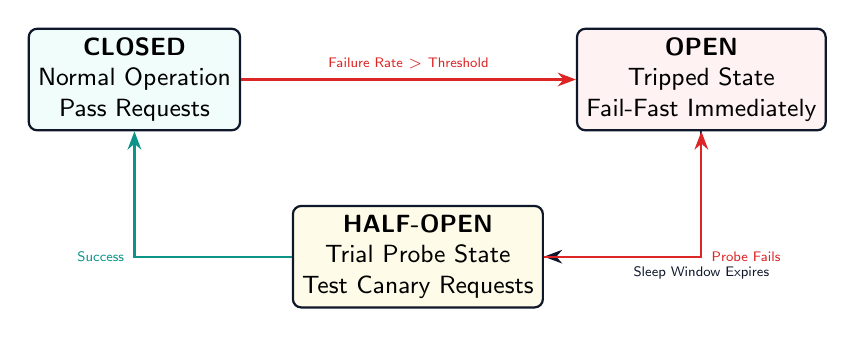
\begin{tikzpicture}[
  scale=0.9,
  state/.style={rectangle, draw=headingblue, fill=codebg, thick, rounded corners=3pt, minimum width=2.6cm, minimum height=1.2cm, align=center, font=\sffamily\small}
]
  \node[state, fill=intuitionBg] (closed) at (0, 0) {\textbf{CLOSED}\\Normal Operation\\Pass Requests};
  \node[state, fill=warningBg] (open) at (8, 0) {\textbf{OPEN}\\Tripped State\\Fail-Fast Immediately};
  \node[state, fill=mistakeBg] (half) at (4, -2.5) {\textbf{HALF-OPEN}\\Trial Probe State\\Test Canary Requests};

  \draw[-{Stealth[scale=1.0]}, thick, color=warningRed] (closed) -- node[above, font=\sffamily\tiny] {Failure Rate $>$ Threshold} (open);
  \draw[-{Stealth[scale=1.0]}, thick, color=headingblue] (open) |- node[below, font=\sffamily\tiny] {Sleep Window Expires} (half);
  \draw[-{Stealth[scale=1.0]}, thick, color=intuitionTeal] (half) -| node[left, font=\sffamily\tiny] {Success} (closed);
  \draw[-{Stealth[scale=1.0]}, thick, color=warningRed] (half) -| node[right, font=\sffamily\tiny] {Probe Fails} (open);
\end{tikzpicture}
\caption{Circuit Breaker Finite State Machine}
\label{fig:circuit-breaker}
\end{figure}

\begin{itemize}[leftmargin=18pt]
  \item \textbf{Closed}: All requests pass through. The breaker tracks sliding-window failure rates (e.g., HTTP 5xx responses or timeouts).
  \item \textbf{Open}: When the error rate exceeds a threshold (e.g., 50\% over 10 seconds), the circuit trips to \textbf{Open}. For the duration of a sleep window (e.g., 30 seconds), all incoming calls \textbf{fail fast immediately} (returning an instant fallback or HTTP 503) without dispatching a network packet. This grants the struggling dependency space to recover.
  \item \textbf{Half-Open}: After the sleep window, the circuit allows a limited number of trial requests (canary probes). If they succeed, the circuit resets to \textbf{Closed}; if any probe fails, it trips back to \textbf{Open}.
\end{itemize}

\subsection{The Bulkhead Pattern}

Named after the watertight partitions in ship hulls that prevent a single hull breach from sinking the vessel, the **Bulkhead Pattern** isolates resources (such as thread pools, memory buffers, or database connections) by dependency:

\begin{figure}[htbp]
\centering
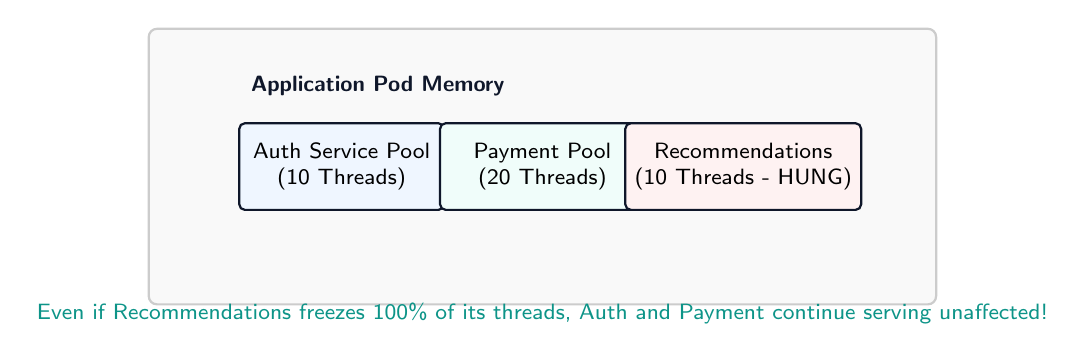
\begin{tikzpicture}[
  scale=0.85,
  box/.style={rectangle, draw=headingblue, fill=codebg, thick, rounded corners=2pt, minimum width=2.6cm, minimum height=1.1cm, align=center, font=\sffamily\footnotesize}
]
  \node[rectangle, draw=gray!40, fill=gray!5, thick, rounded corners=3pt, minimum width=10cm, minimum height=3.5cm] (container) at (4.5, 0) {};
  \node[anchor=north west, font=\sffamily\bfseries\footnotesize, color=headingblue] at (0, 1.5) {Application Pod Memory};

  \node[box, fill=exampleBg] (pool_auth) at (1.5, 0) {Auth Service Pool\\(10 Threads)};
  \node[box, fill=intuitionBg] (pool_pay) at (4.5, 0) {Payment Pool\\(20 Threads)};
  \node[box, fill=warningBg] (pool_rec) at (7.5, 0) {Recommendations\\(10 Threads - HUNG)};

  \node[anchor=south, font=\sffamily\footnotesize, color=intuitionTeal] at (4.5, -2.5) {Even if Recommendations freezes 100\% of its threads, Auth and Payment continue serving unaffected!};
\end{tikzpicture}
\caption{Bulkhead Isolation: Independent Thread Pools per Upstream Service}
\label{fig:bulkhead-isolation}
\end{figure}

\section{Load Shedding and Little's Law}

When incoming traffic overwhelms a service's processing capacity, queuing requests in memory causes response latency to climb exponentially. Under high queuing, requests sit in line so long that by the time they reach execution, the client has already timed out. The server spends 100\% of its CPU processing dead requests!

\subsection{Little's Law and Concurrency Limits}

From queuing theory, Little's Law states:
\begin{equation}
L = \lambda \times W
\end{equation}
where $L$ is the average number of concurrent requests in the system, $\lambda$ is arrival throughput (QPS), and $W$ is the average processing latency.
Every system has an optimal concurrency limit $L_{\text{opt}}$ at which throughput saturates before queue delays degrade latency.

\subsection{Load Shedding Strategies}

\begin{enumerate}[leftmargin=18pt]
  \item \textbf{Token Bucket Concurrency Limiting}: If active in-flight requests exceed $L_{\text{opt}}$, immediately reject excess requests with HTTP 429 (\texttt{Too Many Requests}) or HTTP 503 without enqueuing.
  \item \textbf{CoDel / Queue Timeout Dropping}: If a request has sat in an internal queue for longer than its declared deadline (e.g., $t_{\text{wait}} > 200\text{ ms}$), drop it immediately without executing business logic.
  \item \textbf{Priority Load Shedding}: Categorize requests into tiers:
  \begin{itemize}[leftmargin=12pt]
    \item \textbf{Tier 1 (Critical)}: Checkout, payments, authentication. Never shed.
    \item \textbf{Tier 2 (Standard)}: Search, product details. Shed under severe load.
    \item \textbf{Tier 3 (Non-essential)}: Recommendations, analytics tracking, review posting. Shed immediately at the first sign of CPU saturation.
  \end{itemize}
\end{enumerate}

\section{Chaos Engineering}

Pioneered by Netflix in 2011 with the creation of Chaos Monkey, \textbf{Chaos Engineering} is the discipline of experimenting on a distributed system to build confidence in the system's capability to withstand turbulent conditions in production.

\subsection{The Principles of Chaos Engineering}

\begin{enumerate}[leftmargin=18pt]
  \item \textbf{Define Steady State}: Quantify normal behavior using measurable business metrics (e.g., completed checkouts per minute, p99 latency $< 120\text{ ms}$), not just CPU percentages.
  \item \textbf{Formulate a Hypothesis}: State: \emph{``Even if an entire availability zone loses power, the checkout completion rate will not drop by more than 1\%.''}
  \item \textbf{Inject Realistic Faults}:
  \begin{itemize}[leftmargin=12pt]
    \item Terminate random server instances or pods (Chaos Monkey).
    \item Introduce packet loss, latency, or corrupted packets on network interfaces using Linux \texttt{tc} (Traffic Control) / \texttt{netem}.
    \item Drain availability zones or sever cross-region fiber links.
  \end{itemize}
  \item \textbf{Verify Steady State}: Compare steady-state metrics against the hypothesis.
  \item \textbf{Minimize Blast Radius}: Run experiments in staging or with small production canary traffic before scaling up.
\end{enumerate}

\section{Summary \& Key Takeaways}
\begin{itemize}[leftmargin=18pt]
  \item The $\varphi$-Accrual Failure Detector replaces fragile binary heartbeat timeouts with an adaptive, continuous suspicion scale calculated from historical heartbeat distributions.
  \item Naive retries during degradation trigger catastrophic retry storms, exponentially multiplying traffic against struggling dependencies.
  \item Full Jitter ($\text{rand}(0, \text{Base} \times 2^{\text{attempt}})$) uniformly flattens retry spikes and eliminates thundering herds.
  \item Circuit Breakers fail fast during downstream outages, allowing degraded dependencies time to recover without holding connection pools.
  \item Bulkheads isolate thread pools and resources per dependency, preventing a slow ancillary service from crashing the entire host.
  \item Load shedding enforces Little's Law, shedding low-priority or expired requests to maintain steady-state throughput under extreme traffic spikes.
  \item Chaos Engineering proactively validates resilience hypotheses by injecting real-world failures into production environments under controlled blast radiuses.
\end{itemize}

\section{Exercises}

\subsection{Mechanics}
Write an exponential backoff retry loop in Python that executes up to 5 attempts using AWS Full Jitter with a base delay of $100\text{ ms}$ and a maximum cap of $5{,}000\text{ ms}$.

\subsection{Debugging}
An API gateway connects to a downstream user profile microservice. The gateway has a timeout of $2{,}000\text{ ms}$ and an in-memory thread pool of 200 workers. The user profile service's latency increases from $50\text{ ms}$ to $2{,}500\text{ ms}$. Within 15 seconds, all other routes on the API gateway (including payments and cart) begin timing out with HTTP 504. Explain why and provide the architectural fix.

\subsection{Architecture}
Design an end-to-end resilience architecture for an e-commerce platform during Black Friday. Detail the placement of Circuit Breakers, Bulkheads, Token-Bucket Concurrency Limits, Priority Queue Shedding, and Chaos Engineering game day scenarios.

\section{Detailed Solutions}

\subsection{Solution to Mechanics Exercise}
\begin{lstlisting}[language=Python]
import random
import time

def execute_with_full_jitter(func, max_attempts: int = 5, base_ms: float = 100, cap_ms: float = 5000):
    for attempt in range(max_attempts):
        try:
            return func()
        except Exception as e:
            if attempt == max_attempts - 1:
                raise e

            # Full Jitter formula: rand(0, min(Cap, Base * 2^attempt))
            exponential_ceiling = min(cap_ms, base_ms * (2 ** attempt))
            sleep_ms = random.uniform(0, exponential_ceiling)
            time.sleep(sleep_ms / 1000.0)
\end{lstlisting}

\subsection{Solution to Debugging Exercise}
\textbf{The Thread Pool Exhaustion Cascade:}
\begin{enumerate}[leftmargin=18pt]
  \item The API gateway uses a single shared thread pool of 200 workers for all routes.
  \item When the profile service latency jumps to $2{,}500\text{ ms}$, requests targeting profile wait for the gateway's full $2{,}000\text{ ms}$ timeout before failing.
  \item Because incoming profile requests arrive faster than they time out, all 200 worker threads quickly become occupied waiting for socket reads on the profile service.
  \item Once all 200 threads are blocked, incoming requests for completely unrelated healthy services (payments, cart) cannot acquire a worker thread and are queued or rejected, crashing the entire gateway.
\end{enumerate}
\textbf{The Architectural Fix:}
1. \textbf{Bulkhead}: Allocate dedicated thread pools or non-blocking async clients per downstream dependency (e.g., maximum 20 threads for profile service).
2. \textbf{Circuit Breaker}: Wrap the profile client in a circuit breaker. When 50\% of profile requests hit the 2-second timeout, trip to Open and fail fast in $0\text{ ms}$.

\subsection{Solution to Architecture Exercise}
\textbf{End-to-End Resilience Topology:}
\begin{figure}[htbp]
\centering
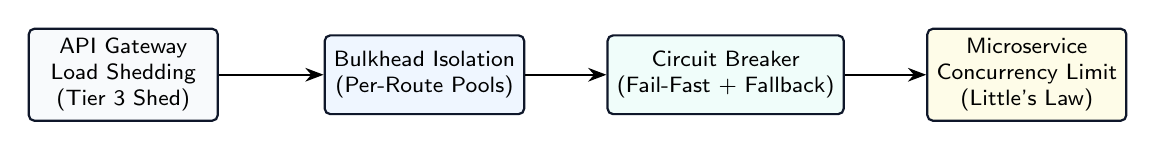
\begin{tikzpicture}[
  scale=0.85,
  box/.style={rectangle, draw=headingblue, fill=codebg, thick, rounded corners=2pt, minimum width=2.4cm, minimum height=1.0cm, align=center, font=\sffamily\footnotesize}
]
  \node[box] (edge) at (0, 0) {API Gateway\\Load Shedding\\(Tier 3 Shed)};
  \node[box, fill=exampleBg] (bulkhead) at (4.5, 0) {Bulkhead Isolation\\(Per-Route Pools)};
  \node[box, fill=intuitionBg] (cb) at (9, 0) {Circuit Breaker\\(Fail-Fast + Fallback)};
  \node[box, fill=mistakeBg] (service) at (13.5, 0) {Microservice\\Concurrency Limit\\(Little's Law)};

  \draw[-{Stealth[scale=1.0]}, thick] (edge) -- (bulkhead);
  \draw[-{Stealth[scale=1.0]}, thick] (bulkhead) -- (cb);
  \draw[-{Stealth[scale=1.0]}, thick] (cb) -- (service);
\end{tikzpicture}
\end{figure}

\begin{enumerate}[leftmargin=18pt]
  \item \textbf{Ingress Priority Shedding}: The API Gateway monitors CPU and queue depth. If CPU $> 85\%$, immediately drop Tier 3 requests (recommendations) with HTTP 429.
  \item \textbf{Bulkheads}: Separate thread and connection pools for Payment (50 connections), Orders (50 connections), Catalog (30 connections).
  \item \textbf{Circuit Breakers}: Deployed on all internal RPC clients. Tripped after 30\% failure rate over 5 seconds; falls back to cached responses or default static recommendations.
  \item \textbf{Adaptive Concurrency Limits}: Services enforce Little's Law using Vegas or gradient concurrency limit algorithms. If latency rises, the concurrency window dynamically contracts, shedding excess traffic at the front door.
  \item \textbf{Chaos Engineering Game Days}: Execute Chaos Monkey AZ termination drills two weeks before Black Friday to verify automated DNS failover and cache stampede protections under production loads.
\end{enumerate}

\section{Further Reading \& Citations}
\begin{itemize}[leftmargin=18pt]
  \item Hayashibara, N., et al. (2004). \emph{The $\varphi$-accrual failure detector}. In Proceedings of the 23rd IEEE International Symposium on Reliable Distributed Systems (SRDS), 66--78.
  \item Brooker, M. (2015). \emph{Exponential Backoff And Jitter}. AWS Architecture Blog. Available at \url{https://aws.amazon.com/blogs/architecture/exponential-backoff-and-jitter/}.
  \item Nygard, M. T. (2018). \emph{Release It!: Design and Deploy Production-Ready Software}. Pragmatic Bookshelf.
  \item Rosenthal, C., et al. (2020). \emph{Chaos Engineering: System Resiliency in Practice}. O'Reilly Media.
\end{itemize}


\backmatter

\end{document}
